%%%%%%%%%%%%%%%%%%%%%%%%%%%%%%%%%%%%%%%%%%%%%%%%%%%%%% SETTINGS %%%%%%%%%%%%%%%%%%%%%%%%%%%%%%%%%%%%%%%%%%%%%%%%%%%%%%%%%%%%%
%clear; bibtex main.aux;pdflatex main.tex ;evince main.pdf &

\documentclass[final,12pt]{report} 						% list options between brackets [draft]

\pdfminorversion = 5									% changing the default PDF version

\usepackage[utf8]{inputenc}								% list packages between braces
\usepackage{graphicx,keystroke}							% colors, scaling and rotation of EPS files (convert file.jpeg file.eps)
\usepackage[frenchb]{babel}								% french as main language
\usepackage[left=0.80in, right=0.80in, top=1.0in, bottom=1.0in]{geometry}		% define margin
\usepackage{verbatim} 									% LaTeX multiline comments
\usepackage{subfig}										% Enable sub figures
\usepackage{amsmath,epsfig}								% Formula
\usepackage[T1]{fontenc}								% pipe... symbol
\usepackage{fancyhdr}									% header, footer
\usepackage{hyperref}									% URL
\usepackage[hyperpageref]{backref}						% Adds ‘backlink’ text to the end of each item in the bibliography
\usepackage{natbib}										% Reimplement the LATEX \cite command
\usepackage{amssymb}									% American Mathematical Society symbol Real En	
\usepackage[toc,page,titletoc]{appendix}				% 
\usepackage[toc,xindy]{glossaries}						% Use glossaries


%\usepackage{multirow}									% tabular addition
%\usepackage{normalem}									% Overwrite \emph and permit barred text, special underlining...

%\usepackage{tikz}
%\usepackage{kpfonts}
%\usepackage[explicit]{titlesec}

								% Custom packages		

\makeatletter

\renewcommand{\maketitle}{%
{
	\pagestyle{empty}
\begin{center}

	%\includegraphics[width=2cm]{fig/logo_UnivLR2011.png}\\
	\bigskip
	
	\begin{LARGE}
		Scientific report\\
		%Master Recherche en Systèmes Dynamiques et Signaux\\
	\end{LARGE}\bigskip
	
	\begin{large}
		First year PhD report\\
		%Année 2010-2011\\
	\end{large}\bigskip\bigskip
	
%	\begin{LARGE}
%		Rapport bibliographique intermédiaire\\% de Master 2 Recherche SDS:\\
%	\end{LARGE}\bigskip
	
	\begin{large}
		\href{http://www.christophe-rigaud.com}{Christophe RIGAUD}\\
	\end{large}\bigskip\bigskip

	\begin{normalsize}
		September 28, 2012\\
	\end{normalsize}\medskip
	
	\begin{normalsize}
		%L3i lab, University of La Rochelle\\
		%LISA - ISTIA - 62 avenue Notre-Dame du Lac 49000 ANGERS\\\bigskip
		\bigskip\bigskip\bigskip\bigskip\bigskip\bigskip\bigskip\bigskip\bigskip
	\end{normalsize}
	
	\begin{Large}
		\bf{Segmentation and indexation of complex object: application to the detection and recognition of complex objects in comics books}
		\bigskip\bigskip\bigskip\bigskip\bigskip\bigskip\bigskip\bigskip\bigskip
	\end{Large}
	
	\begin{normalsize}
		Supervisors:\\
	\end{normalsize}
	\parbox{15cm}{
		\begin{tabbing}
			Dr. Jean-Christophe BURIE\hspace{5em}\= Professor at University of La Rochelle\\
			Pr. Jean Marc OGIER\> Professor and director of L3i lab\\
				%\> F. Chapeau Blondeau	\> Professeur Université d'Angers\\
				%\> J.L. Boimond			\> Professeur Université d'Angers\\
				%\> M. Bourcerie			\> Professeur Université d'Angers\\
				%\> P. Declerck			\> MCF Université d'Angers\\
				%\> J.B. Fasquel  		\> MCF Université d'Angers\\
				%\> C. Jean-Guillaume	\> MCF Université d'Angers\\
				%\> M. Lhommeau			\> MCF Université d'Angers\\
				%\> D.Rousseau			\> MCF Université d'Angers
		
		\end{tabbing}
	}
	\bigskip\bigskip\bigskip
\end{center}
%	\begin{large}
%		Encadrant: Jean-Baptiste FASQUEL		
%	\end{large}

\begin{minipage}{0.5\textwidth}
\begin{flushleft}
    \includegraphics[width=2cm]{fig/logo_UnivLR2011.png}\\
    Technoforum \\
    Université de La Rochelle \\
    23, avenue Albert Einstein \\
    17071 La Rochelle - Cedex 9 - France
\end{flushleft}
\end{minipage}
\begin{minipage}{0.5\textwidth}
\begin{flushright}
    \includegraphics[width=4cm]{fig/L3I-LOGO-quadri1.jpg}\\
    Pôle Sciences et Technologies \\
    Université de La Rochelle\\    
    Avenue M. Crépeau\\	
    17042 La Rochelle - Cedex 01 - France
\end{flushright}
\end{minipage}


		\clearpage
	}
}

%\def\thechapter{\Roman{chapter}} 
%\def\thesection{\arabic{section}} 
        
% Chapter (general)
\def\@makechapterhead#1{%
  {\parindent \z@ \raggedright \normalfont
    \ifnum \c@secnumdepth >\m@ne
        %\huge\bfseries \@chapapp\space \thechapter
        \par\nobreak
        \vskip 20\p@
    \fi
    \interlinepenalty\@M
    \Huge \bfseries \thechapter \hspace{0.2em} #1 \par\nobreak
    \vskip 30\p@			% space under chapter name
  }}

% Chapter table of content
\def\@makeschapterhead#1{%
  {\parindent \z@ \raggedright
    \normalfont
    \interlinepenalty\@M
    \Huge \bfseries  #1\par\nobreak
    \vskip 40\p@			% space under "table of content"
  }}



\makeatother
								% Custom commands

%----------------------------------------------
%HEADER
\pagestyle{fancy}
\fancyhead{} 															% Clear all header fields
\fancyhead[RO,RE]{\includegraphics[height=30pt]{pic/pic\thepage.png}}	% Right Odd AND Right Even 
\fancyhead[LO,LE]{\rightmark}											% Left Odd AND Left Even

\fancyfoot{}															% Clear all foot fields
%\fancyfoot[L]{Christophe Rigaud}
\fancyfoot[C]{}
\fancyfoot[R]{\thepage}
%\fancyfoot[L]{\href{http://www.christophe-rigaud.com}{Christophe Rigaud}}

%----------------------------------------------
%LINK AND WINDOW
\hypersetup{
    colorlinks,
    citecolor=black,
    filecolor=black,
    linkcolor=black,
    urlcolor=black,
    unicode=false,          					% non-Latin characters in Acrobat’s bookmarks
    pdftoolbar=true,        					% show Acrobat’s toolbar?
    pdfmenubar=true,        					% show Acrobat’s menu?
    pdffitwindow=false,    						% window fit to page when opened
    pdfstartview={FitH},    					% fits the width of the page to the window
    pdftitle={Rapport de Master Recherche Mathématiques et Applications - Christophe Rigaud - 2011},    % title
    pdfauthor={Christophe Rigaud},     			% author
    pdfsubject={Interprétation d'images et graphe conceptuel intégrant des connaissances topologiques et photométriques},   			% subject of the document
    pdfcreator={Christophe Rigaud},   			% creator of the document
    pdfproducer={pdflatex}, 			% producer of the document
    pdfkeywords={Traitment d'image} {graphe conceptuel} {conceptuel} {topologie} {photométrie} {christophe rigaud}, % list of keywords
    pdfnewwindow=true      						% links in new window
}
%\hypersetup{
%	%DOC : http://www.tug.org/applications/hyperref/manual.html
%    %bookmarks=true,        % show bookmarks bar?
%    unicode=false,          % non-Latin characters in Acrobat’s bookmarks
%    pdftoolbar=true,        % show Acrobat’s toolbar?
%    pdfmenubar=true,        % show Acrobat’s menu?
%    pdffitwindow=false,     % window fit to page when opened
%    pdfstartview={FitH},    % fits the width of the page to the window
%    pdftitle={Rapport de Master - Christophe Rigaud},    % title
%    pdfauthor={Christophe Rigaud},     			% author
%    pdfsubject={Traitement d'image},   			% subject of the document
%    pdfcreator={Christophe Rigaud},   			% creator of the document
%    pdfproducer={Christophe Rigaud}, 			% producer of the document
%    pdfkeywords={image} {conceptuel} {méthode}, % list of keywords
%    pdfnewwindow=true,      % links in new window
%%    colorlinks=false,       % false: boxed links; true: colored links
%    linkcolor=black,          % color of internal links
%%    citecolor=green,        % color of links to bibliography
%%    filecolor=magenta,      % color of file links
%%    urlcolor=green          % color of external links
%}

%----------------------------------------------
% Document settings

%\setcounter{secnumdepth}{3} %subsubsections are numbered
%\setcounter{tocdepth}{3} %subsubsections are added to the TOC

%\renewcommand{\tocbibname}{References} 

\hyphenation{li-mi-terons i-ma-ges in-flu-ence}

%----------------------------------------------
%Alter page dimensions

%\setlength{\textwidth}{16cm}
%\setlength{\oddsidemargin}{0.46cm}
%\setlength{\evensidemargin}{0.46cm}
%\setlength{\textheight}{22.3cm}
%\setlength{\topmargin}{-0.54cm}
%\setlength{\headsep}{1.5cm}
%\setlength{\footnotesep}{0.6cm} 



									% Custom styles

%%%%%%%%%%%%%%%%%%%%%%%%%%%%%%%%%%%%%%%%%%%%%%%%%%%%%% DOCUMENT %%%%%%%%%%%%%%%%%%%%%%%%%%%%%%%%%%%%%%%%%%%%%%%%%%%%%%%%%%%%%

\makeglossaries
\newglossaryentry{ROI}{name={ROI}, description={app Domain Description...}}
%\newglossaryentry{sample}{name={has been inserted aaa},description={testing testing 123}}
%\newglossaryentry{topologie}{description={La topologie est une branche des mathématiques concernant l'étude des déformations spatiales par des transformations continues (sans arrachages ni recollement des structures)\url{http://fr.wikipedia.org/wiki/Topologie}}
%\newglossaryentry{Moteur d'inférence, de l'anglais "enference engine" et du verbe « inférer » qui signifie « déduire », c'est un concept de raisonnement déductif, qui peut être concrètement un logiciel, à qui on demande des informations et qui essaye de les déduire à partir de sa base de connaissances.})
%\footnote{Le fenêtrage est le fait de considérer qu'une fraction de la dynamique d'une image (exemple : un intervalle dans un histogramme d'image), on l'utilise souvent pour faciliter la visualisation ou les traitements d'une image.}

\begin{document}
	%--------------------------------------------------------------------------------------------------
	\renewcommand{\labelitemi}{$\bullet$}
	\renewcommand{\appendixtocname}{Annexes}
	\newcounter{ale}
	\setcounter{tocdepth}{4}

	%--------------------------------------------------------------------------------------------------
	\maketitle
	%--------------------------------------------------------------------------------------------------
	\newpage
	\vspace*{\fill}
%	\begin{center}
%		Cette page est laissée blanche intentionnellement.
%	\end{center}
%	\vspace{\fill}
	\hspace{1em}Je soussigné Christophe Rigaud déclare être pleinement conscient que le plagiat de documents ou
d’une partie d’un document publiés sur toutes formes de support, y compris l’internet, constitue une violation
des droits d’auteur ainsi qu’une fraude caractérisée. 
En conséquence, je m’engage à citer toutes les sources
que j’ai utilisées pour écrire ce rapport.\vspace{1em}

Signature :

	\thispagestyle{empty}
	%--------------------------------------------------------------------------------------------------
	\newpage	
%	
\begin{abstract}

	Mots clés : interprétation d'image, fenêtrage, moteur d'inférence, topologie, photométrie.\\

	Ce rapport fait état de l'art en matière d'interprétation d'image guidée par des connaissances topologiques et photométriques à priori. L'utilisation d'informations à priori est un moyen d'anticiper le contenu d'une image et donc d'en optimiser son traitement. On représente ces connaissances sous forme de graphes conceptuels à partir desquels on infère le contenu de l'image. Il s'agit plus concrètement du nombre de classes de l'image et de leurs relations photométriques, à tout instant d'une procédure de segmentation itérative. Un point important de notre étude est la limitation à des connaissances non quantitatives de manière à appliquer un traitement spécifique à chaque image et à prendre en compte ses particularités.

	Dans un second temps, nous quantifions les bénéfices de la méthode proposée à savoir, la diminution des données polluantes, le gain de temps de calcul ou encore sa robustesse.
	
	Une dernière partie est consacrée à l'application à des images médicales de la région de l'abdomen dans lesquelles on fait apparaître clairement les tumeurs du foie et les vaisseaux hépatiques dans le but d'assister le diagnostic médical.


\vspace{5em}

	Keywords: image interpretation, windowing, inference engine, topology, photometry.\\

	This report is the state of the art of image interpretation led by topological and photometrical informations. Using a priori informations is a method to anticipate the content of an image and then to improve the processing. We represent these informations as conceptual graphs and we infer image content. It is more precisely the number of classes in the image and their photometric relations, at each iteration of a segmentation procedure. One important point is that we consider only non quantitative informations in order to specify the image processing and consider its particularity.
	
	Then we quantify the benefits of the proposed method namely polluted data reduction, processing time improvement and strength.
	
	The last part of this work is an application to medical images from abdomen that we proceed in order to show clearly liver tumors and vessel system for diagnostic assistance purpose.
 	
\end{abstract}

	
	\chapter*{Remerciements}
	\vspace*{\fill}
%	\fbox{ %fbox est utilisé pour voir les bords de la minipage
%	\begin{minipage}[c]{15cm}
%	\begin{center}

	{\it
	Je tiens à remercier le laboratoire LISA, son directeur Jean Louis Boimond, les enseignant-chercheurs, les doctorants et les administratifs de m'avoir accueilli et épaulé tout au long de ce stage.\vspace{1em}
	
	Je remercie plus particulièrement mon tuteur de stage, Jean-Baptiste Fasquel, pour la richesse du sujet proposé, l'encadrement irréprochable, sa disponibilité et la correction de ce rapport.\vspace{1em}
	
	Merci également à Laurent Hardouin pour la qualité des enseignements et l'encadrement de ce master SDS. Je n'oublie pas le soutien pour une poursuite en doctorat qu'il m'a apporté, tout comme mon tuteur.\vspace{1em}
	
	J'adresse un clin d'\oe{}il particulier à mes chers collègues de laboratoire qui ont, malgré la différence de parcours, su contribuer à une ambiance de travail exceptionnelle. Merci à Antoine, Alban, Floran, Gheotry, Yann et Vincent.
	
	}

%	\end{center}
	\vspace{\fill}


%	TO DO\\
%Encadrement
%	- Fasquel : disponibilité
%	- Hardoin : gestion
%	
%Recherche de thèse
%	- J.B.Fasquel : lettre, conseil
%	- L. Hardouin : lettre
%	- L. Autrique : conseil, contact
%	- F. Chapeau Blondeau : analyse des production scientifiques
	
%Collègues
%	- SDS : soutient moral et bonne ambiance
%	- PSI : intégration, bonne ambiance

 
	\thispagestyle{empty} 								%get rid of header/footer for toc page
	%--------------------------------------------------------------------------------------------------
	\tableofcontents 									%put toc in
	\thispagestyle{empty} 								%get rid of header/footer for toc page
%	\cleardoublepage 									%start new page
%	\pagestyle{plain} 									% put headers/footers back on
	\setcounter{page}{0} 								%reset the page counter
	%--------------------------------------------------------------------------------------------------
	%COMPILATION: 
%clear; bibtex main.aux;pdflatex main.tex ;evince main.pdf &

\chapter{Introduction}                   		% chapter 1 
	\section{Contexte et objectif}

	Les travaux présentés dans ce document ont été réalisés au cours d'un stage de master recherche de cinq mois qui s'est déroulé au sein du laboratoire LISA de l'école d'ingénieur ISTIA à Angers. Plus particulièrement dans le contexte de l'activité de recherche de l'analyse d'images pour l'aide au diagnostic. Il fait suite à une recherche bibliographique sur ``l'interprétation d'images et graphe conceptuel intégrant des connaissances topologiques et photométriques''. 
	
	L'objectif de ce stage est d'utiliser des notions conceptuelles non quantitatives, topologiques et photométriques, pour l'interprétation d'images synthétiques puis médicales.
	Le bénéfice attendu est d'optimiser la segmentation et le fenêtrage\footnote{Le fenêtrage est le fait de considérer qu'une fraction de la dynamique d'une image (e.g. une section d'un histogramme d'image), on l'utilise souvent pour faciliter la visualisation ou les traitements d'une image.} (rendu visuel) d'une région d'intérêt (e.g. tumeur).
	
	%Il est le fruit d'une centaine d'heures de documentation et de réflexion sur l'intégration de connaissances spatiales (e.g. distance, topologie \footnote{La topologie est une branche des mathématiques concernant l'étude des déformations spatiales par des transformations continues (sans arrachages ni recollement des structures)\url{http://fr.wikipedia.org/wiki/Topologie}.}) et photométriques pour l'interprétation des images (i.e. segmentation et identification de régions). L'objectif est d'intégrer ce type de notion conceptuelle ou abstraite en privilégiant celles qui ne sont pas quantitatives (topologie, relation d'intensité non quantitative). Le bénéfice attendu est de faciliter le paramétrage d'algorithmes utilisés pour l'interprétation d'images et la réduction de l'espace de recherche (ex. région d'intérêt). Ce travail fait suite aux travaux de M.Fasquel \cite{Fasquel2006} qui se limitait aux informations topologiques, avec pour application l'analyse d'images médicales pour l'aide au diagnostic.

%{\bf Trop particulier: pour des actes diagnostic spécifique (recherche de tumeur...)}

%{\bf La phrase "Ces connaissances sont souvent représentées sous forme de graphe conceptuel." a été retirée car trop spécifique (éventuellement à placer ailleurs).}

% , sur l'interprétation séquentielle d'images et de graphes conceptuels pour l'optimisation du fenêtrage \footnote{Le fenêtrage est le fait de considérer qu'une fraction de la dynamique d'une image (exemple : un intervalle dans un histogramme d'image), on l'utilise souvent pour faciliter la visualisation ou les traitements d'une image.} d'images médicales. Ce fenêtrage pourra être effectué au moyen d'un logiciel permettant à l'utilisateur d'interagir avec des images numériques.
%Le thème est original par la combinaison de deux bases de connaissances à priori indépendantes, à caractère topologique et photométrique. Il fait suite aux travaux de M.Fasquel \cite{Fasquel2006}. Le cadre général est le développement de méthodes et d'outils d'assistance au diagnostic.

	\section{Problématique}
	
	Nous proposons d'interpréter des images en combinant des informations topologiques \cite[Fasquel]{Fasquel2006} et photométriques non quantitatives. Un exemple de situation où ce type d'information pourrait être avantageusement exploité serait celui illustré par la figure~\ref{fig:sl_0_1}. Cet exemple concerne le rendu volumique d'une image médicale. Le choix de la fenêtre de rendu (une plage d'intensités à afficher) est crucial pour améliorer la perception d'une structure donnée. Dans ce cas, on cherche à rendre le réseau vasculaire, supposant que l'on dispose du masque des os. Sachant que le réseau vasculaire n'est pas inclus dans les os (information topologique à priori), on peut tout simplement retirer de l'image le volume relatif au os afin de faciliter la visualisation du réseau vasculaire (figure~\ref{fig:sl_0_2}). Par ailleurs, dans l'hypothèse où le réseau vasculaire est plus clair que le tissu du foie (information photométrique que l'on retrouve visuellement sur la figure~\ref{fig:sl_0_2}), on peut modifier le fenêtrage de manière à afficher que les tissus qui ont une intensité supérieure à ceux du foie (voir figure~\ref{fig:sl_0_3}).

	%%%%%%%%%%%%%%%%%%%%%%%%%%%%%%%%%%%%%%%%%%%%%%%%
	\begin{figure}[!ht]	%trim=l b r t  width=0.5\textwidth, 
	  \centering
		\subfloat[Rendu initial]{\label{fig:sl_0_1}\includegraphics[trim= 0mm 15mm 0mm 10mm, clip, height=0.24\textwidth]{Introduction/figure/sl_0_1.png}}					\hspace{0.4em}
		\subfloat[Rendu intermédiaire (masquage)]{\label{fig:sl_0_2}\includegraphics[trim= 0mm 15mm 0mm 15mm, clip, height=0.24\textwidth]{Introduction/figure/sl_0_2.png}}	\hspace{0.4em}
		\subfloat[Rendu optimal (fenêtrage)]{\label{fig:sl_0_3}\includegraphics[trim= 5mm 20mm 5mm 15mm, clip, height=0.24\textwidth]{Introduction/figure/sl_0_3.png}}
		\caption{Rendu manuel du réseau vasculaire}
	\end{figure}
	%%%%%%%%%%%%%%%%%%%%%%%%%%%%%%%%%%%%%%%%%%%%%%%%
	
%\newpage
	Cet exemple peut nous amener à nous poser les questions suivantes :\vspace{1 em}

	Si l'on considère une image en niveaux de gris, contenant une région $A$ et une région $B$ comme sur la figure~\ref{fig:structure_a_b}, comment représenter et utiliser, pour l'interprétation automatique d'images, des concepts non quantitatifs tels que :


	\begin{itemize}
		\item La région $A$ recouvre-t-elle la région $B$ (topologie)?
		\item La région $A$ est-elle plus claire que la région $B$ (photométrie)?
	\end{itemize}
\vspace{1em}

Quels en sont les bénéfices?


	\begin{figure}[!ht]
	  \centering
	      \includegraphics[width=0.2\textwidth]{Introduction/figure/structures_a_b.png}
	  \caption{Représentation synthétique des régions.}
	  \label{fig:structure_a_b}
	\end{figure}


	On s'intéressera à ces questions dans le cas d'un processus d'interprétation séquentiel de l'image où chaque étape conduira à la compréhension d'une région de l'image (i.e. segmentation et identification). Compte tenu de ces questions, la problématique de notre travail peut être modélisée par la figure suivante : 
	%\les aspects sous-jacents à traiter concernent:\\
	
	\begin{figure}[!h]
	\setlength{\unitlength}{1mm}
	\begin{center}
	\begin{picture}(60,40)
		\put(-10,0){\framebox(80,10){Guidage du traitement de l'image}}
		\put(30,15){\vector(0,-2){5}} 
% 		\put(30,10){\vector(0,0){5}} 
		\put(-10,15){\framebox(80,10){Moteur d'inférence (déduction)}}
		\put(40,30){\vector(0,-2){5}}
		\put(20,30){\vector(0,-2){5}}
% 		\put(30,25){\vector(0,0){5}}  
		\put(32,30){\framebox(90,10){Modélisation du processus de segmentation}}
		\put(-62,30){\framebox(90,10){Représentation des informations conceptuelles}}
	\end{picture}
	\end{center}
	\caption{Problématique et entités associées.}
	\label{pic:process1}
	\end{figure} 


%	\begin{itemize}
%	\item La représentation de ces informations
%	\item La modélisation du processus de segmentation
%	\item Les inférences (déductions à partir du graphe portant sur la région d'intérêt et les classes)
%	\item L'utilisation pour guider le traitement de l'image \\
%	\end{itemize}

%	La problématique de notre travail est modélisée par la figure suivante : \\

	  \section{État de l'art}
	  \label{sec:state_of_the_art}

	%%%%%%%%%%%%%%%%%%%%%%%%%%%%%%%%%%%%%%%%%%%%%%%%%%%%%%%%%%%%%%%%%%%%%%%%%%%%%%%%%%%%%%%%%%%%%%%%%%%%%%%%%%%%%%%%%%%%%
	%													État  de l'art													%
	%%%%%%%%%%%%%%%%%%%%%%%%%%%%%%%%%%%%%%%%%%%%%%%%%%%%%%%%%%%%%%%%%%%%%%%%%%%%%%%%%%%%%%%%%%%%%%%%%%%%%%%%%%%%%%%%%%%%%
		\subsubsection*{Stratégie d'analyse d'image}
	Plusieurs approches de segmentations automatiques d'images ont déjà ét{\bf é} mises à l'épreuve. La première consiste à considérer l'image dans son ensemble. L'idée est de concevoir un seul algorithme permettant de segmenter toutes les structures d'une image \citep[Moreno]{Moreno2008}\citep[Kobashi]{Kobashi1995}. Il est néanmoins courant que toutes les régions d'une images ne puissent pas être segmentées avec un seul algorithme. Il est donc souvent plus réaliste de concevoir un algorithme spécifique à chacune des structures : c'est l'approche séquentielle ou itérative. Elle consiste à segmenter les structures les une après les autres avec un algorithme spécifique à chacune d'elles. Pour segmenter une structure donnée, il est pertinent de s'appuyer sur les informations relatives aux structures préalablement segmentées. Typiquement, il peut s'agir de l'intégration d'une région d'intérêt permettant de délimiter une zone de recherche pour la structure à segmenter \citep[Hudelot]{Hudelot2008}\citep[Fasquel]{Fasquel2006}.


		\subsubsection*{Informations conceptuelles}
	L'utilisation d'informations à priori est un moyen d'anticiper le contenu d'une image et donc d'en optimiser son traitement. En analyse d'image guidée par des informations à priori abstraites, les travaux récemment réalisés se focalisent sur des informations spatiales. Il peut s'agir de relations entre les structures de type topologiques (e.g. inclusion, recouvrement, adjacence) \citep[Fasquel]{Fasquel2006}\citep[Egenhofer]{Egenhofer2009}\citep[Hudelot]{Hudelot2008} ou bien relatives à des notions de direction et de distance \citep[Hudelot]{Hudelot2008}. Un inconvénient des informations de distance et de direction est leurs aspects quantitatifs. Ceci implique la détermination de paramètres qui doivent être adaptés à l'application considérée. Ceci est notamment le cas des récents travaux de \citep[Hudelot]{Hudelot2008}, ou les informations de distance et de direction sont manipulées en utilisant la logique floue, ceci induisant une phase d'apprentissage \textit{``fuzzy model learning''}.


	Ces représentations conceptuelles (ontologiques\footnote{L'ontologie constitue en soi un modèle de données représentatif d'un ensemble de concepts dans un domaine, ainsi que des relations entre ces concepts. ``L'ontologie est aux données ce que la grammaire est au langage'' \url{http://fr.wikipedia.org/wiki/Ontologie_(informatique)}} \citep[Atif]{Atif2007}) sont encore peu étudiées en interprétation d'image \textit{``the development of ontology-based methods for image interpretation is still in its infancy''} \citep[Hudelot, p.1929]{Hudelot2008}. Il demeure une difficulté majeure lors de leurs applications au niveau des algorithmes d'analyses d'images : \textit{``there still exists a large gap between the semantic interpretation of a medical image and its low-level features'' } \citep[Deruyver, p.1245]{deruyver2009}. Comme récemment souligné dans \citep[Hudelot]{Hudelot2008}, ce type de connaissance est généralement utilisé dans des contextes différents de l'interprétation d'images, tel que l'annotation d'images. 

	A notre connaissance, il n'y a pas eu de travaux relatifs à l'analyse d'images guidée par le couplage d'informations conceptuelles topologiques et photométriques non quantitatives, ceci constituant une première originalité de l'orientation de nos travaux.


	\section{Organisation de l'étude}

	L'étude est organisée selon trois aspects correspondant aux volets : formalisation, évaluation et application. 
Le premier aspect (chapitre 2) est dédié à la formalisation en matière de représentation des connaissances et du moteur d'inférence. En ce qui concerne le moteur d'inférence, il s'agit d'établir les relations permettant de déduire, à partir de connaissances à priori sur l'image, des informations bénéfiques au traitement de l'image. 

Le second aspect (chapitre 3) se focalise sur l'évaluation des bénéfices des informations déduites, dans le cas d'un algorithme particulier, le {\it K-Means clustering}, couramment utilisé en traitement d'images.
Le dernier aspect (chapitre 4) est dédié à l'illustration du bénéfice de ce travail dans un cadre applicatif bien particulier relatif à la visualisation d'images médicales.


%	Nous nous limiterons à deux cas d'utilisations pour appuyer cette étude:
%	\begin{itemize}
%		\item l'interprétation d'images synthétiques ;
%		\item la visualisation optimale d'images médicales par un processus de segmentation interactif. \\
%	\end{itemize}

	%Dans ces deux cas d'utilisations, l'algorithme d'analyse d'images sera basé sur une méthode d'analyse d'histogramme classique à partir duquel on identifiera les différentes régions de l'image (voir figure~\ref{fig:melange}). Le cas de l'interprétation d'images synthétiques a principalement pour objectif d'illustrer la problématique, les différents concepts impliqués, la solution proposée {\bf et d'en évaluer quantitativement les bénéfices}.
%	Dans ces deux cas d'utilisations, l'algorithme d'analyse d'images sera basé sur une méthode classique de partitionnement de points selon leurs intensités et correspondants à différentes structures anatomiques et pathologiques\footnote{La pathologie est l'étude des maladies et de leurs causes. Le terme peut être employé comme un nom pour désigner une anomalie dans un corps.} (voir le schéma figure~\ref{fig:melange}). 
	
%	Le premier cas a principalement pour objectif d'illustrer la problématique, les différents concepts impliqués, la solution proposée et d'en évaluer quantitativement les bénéfices.

%Pour cela, il est nécessaire de reconnaître automatiquement la structure d'intérêt au sein de l'image. Nous présenterons les méthodes de traitement d'image existantes, dans le chapitre suivant.


%	\begin{figure}[!ht]
%	  \centering
%	      \includegraphics[width=0.9\textwidth]{Introduction/figure/information_a_priori.png}
%	  \caption{Classification des informations conceptuelles.}
%         \label{fig:information_a_priori}
%	\end{figure}

%		\subsubsection*{Informations conceptuelles: représentation}
%		\label{sec:info_concept_reps}
%	La représentation des connaissances, en particulier spatiales, peut se baser sur un graphe (conceptuel lorsque l'on parle de connaissances conceptuelles) où les noeuds sont associés aux différentes entités supposées présentes dans l'image. Les arcs reliant les noeuds représentent les relations (e.g. à gauche, à droite, inclus). Ce type de représentation a notamment été récemment considéré par \citep[Deruyver, p.1246]{deruyver2009} et \citep[Fasquel]{Fasquel2006} et facilite la compréhension : ``\textit{Graph techniques permit to represent image objects and scenes in very natural way}'' \citep[Sanfeliu]{Sanfeliu2002}.


%		\subsubsection*{Informations conceptuelles, contextuelles et interprétation séquentielle}
%	Ces informations conceptuelles à priori peuvent être enrichies tout au long du traitement de l'image. Dans \citep[Fasquel]{Fasquel2006}, ces informations deviennent alors contextuelles : les informations à priori, très générales, deviennent davantage spécifique à l'image en cours d'analyse. Les informations contextuelles évoluent en fonction du contexte dans lequel se trouve une image à un moment donné. Par exemple, lors de la segmentation d'une image, les structures déjà segmentées ou encore le nombres de classes (non pas en général, mais compte tenu des structures déjà identifiées), sont des informations contextuelles. Pour représenter cette évolution des connaissances (i.e. connaissances à priori enrichies par les connaissances contextuelles), on peut intégrer la notion d'activation de noeud du graphe conceptuel initial, comme considéré récemment par \citep[Fasquel]{Fasquel2006}.


%	\section{Analyse d'images par seuillage d'histogramme}		%Information photométrique
%	\label{sec:ana_img_by_threshold}
%	Comme ceci a été précisé lors de la présentation de la problématique générale, nous nous limiterons essentiellement à une analyse d'images basée sur le seuillage d'histogramme\footnote{L'histogramme d'une image est un graphique qui associe les niveaux de gris au nombre de pixel dans l'image qui contient ces niveaux de gris.}. Ce choix est notamment justifié par la nature des informations conceptuelles que nous proposons d'étudier, en particulier l'information photométrique. L'information topologique, quand à elle, interviendra pour réduire le calcul de l'histogramme au sein d'une région d'intérêt, afin d'éliminer les données qui pourraient altérer son analyse (e.g. les données correspondant aux régions déjà segmentées).

%	Nous ne prétendons pas, et ce n'est pas l'objectif de cette étude, proposer une méthode de seuillage d'histogramme nouvelle. Il est néanmoins intéressant de souligner qu'il s'agit d'une catégorie d'algorithme couramment utilisés en traitement d'images, et qui font encore  aujourd'hui l'objet d'études afin d'améliorer leur robustesse. Nous en rappelons ci-dessous succinctement le principe et les limitations couramment rencontrées.

%	Le principe du seuillage\footnote{Le seuillage d'image est la méthode la plus simple de segmentation d'image. À partir d'une image en niveau de gris, le seuillage d'image peut être utilisé pour créer une image comportant uniquement deux valeurs, noir ou blanc (monochrome). \url{http://fr.wikipedia.org/wiki/Seuillage_d'image}} d'histogramme consiste à dire qu'un ensemble de pixels, d'une même image, dont l'intensité est comprise dans un certain intervalle, appartiennent à une structure donnée. Il apparaît donc les notions de seuil minimum et maximum de l'intervalle. Plusieurs études sur les méthodes de seuillage d'histogramme d'image ont été réalisées mais il demeure un problème de robustesse lors de la détermination des seuils (\citep[Coudray]{Coudray2010}, \citep[Bhattacharyya]{Bhattacharyya2011}, \citep[Cheng]{Cheng1998}, \citep[Cuevas]{Cuevas2010}). Le lecteur pourra également se référer à l'état de l'art de \citep[Zhang]{Zhang2008} sur ces méthodes.\vspace{1 em}

%	Une des méthodes célèbres à deux niveaux et celle de \citep[Otsu]{Otsu1979} qui déterminent un seuil entre deux classes considérées donc comme l'objet et le fond de l'image.  Il en résulte une image avec deux classes (souvent noir et blanc) dite \textit{``binaire''}. Travailler avec des images binaires est plus simple et donc plus rapide qu'avec des images en niveau de gris car il n'y a que deux couleurs à considérer. Notons tout de même qu'il y a une importante perte d'information par ce fait mais qu'elle peut être négligée si les seuils sont bien choisis. Des extensions récentes, multi-niveaux, existent \citep[Huang 2009]{Huang2009}. Cette même catégorie a été récemment illustré par  \citep[Cuevas]{Cuevas2010} qui considère plusieurs classes inconnues dans l'image et trouve les seuils qui les bornes. D'autre part, il existe des algorithmes de mélange gaussien \textit{``gaussian mixture''} \citep[Gupta]{Gupta1998} (qui ont par ailleurs fait l'objet d'une récente extension \citep[Huang]{Huang2008}), qui permettent d'estimer les paramètres des courbes de Gauss figure~\ref{fig:gauss_mix} (souvent caractéristique de la répartition des intensités d'une structure quelconque).  Nous l'utiliserons dans ce travail.

%	Dans le cas de cet algorithme couramment utilisé, un élément important concerne la connaissance à priori du nombre de classes (ou régions photométriquement distinctes) présentes dans l'image. Ceci détermine le nombre de lobes présentes dans l'histogramme. Un second élément concerne \textit{``l'identité''} ou \textit{``l'étiquette''} de la région associée à chacun de ces lobes. Par exemple, dans le cas d'images médicales anatomiques, il peut s'agir d'associer correctement un lobe donné de l'histogramme à une structure anatomique particulière. L'objectif du travail effectué sera de déterminer automatiquement le nombre de lobes et leurs identités. Ceci se fera par inférence sur la représentation conceptuelle des connaissances à priori et contextuelles. Par rapport à l'application médicale visée, ces informations pourront être utilisées pour déterminer automatiquement le fenêtrage à considérer.


%	\begin{figure}[!ht]
%	  \centering
%	      \includegraphics[width=0.5\textwidth]{Introduction/figure/gauss_param.jpg}
%	  \caption{Estimation de gaussiennes.}
%         \label{fig:gauss_mix}
%	\end{figure}

%\newpage

%	\section{Synthèse}
%	Compte tenu de notre connaissance des travaux existants présentés précédemment, l'originalité de nos travaux concernent principalement les trois points suivants :
%	\begin{itemize}
%		\item
%		l'intégration des connaissances photométriques au modèle existant proposé par \citep[Fasquel]{Fasquel2006};
%		\item
%		l'établissement des relations (inférence) entre cette représentation conceptuelle des connaissances et les paramètres quantitatifs d'un seuillage d'histogramme fondé sur le modèle de mélange de gaussiennes. Ces relations concerneront le nombre de classes attendues dans l'image à un instant \textit{t}, puis la détermination de leurs \textit{``étiquettes''};
%		\item
%		l'illustration de l'intérêt de cette approche pour une application particulière : le fenêtrage d'images médicales.
%	\end{itemize}


	

\chapter{Représentation des connaissances, processus d'analyse et inférence}
\label{chap:info_concept}

    \section{Représentation des connaissances}
    
    	La représentation des connaissances se base sur un graphe conceptuel où les noeuds sont associés aux différentes entités supposées présentes dans l'image. Les arcs reliant les noeuds représentent les relations (e.g. à gauche, à droite, inclus). Ce type de représentation a notamment été récemment considéré par \citep[Deruyver, p.1246]{deruyver2009} et \citep[Fasquel]{Fasquel2006} et facilite la compréhension : ``\textit{Graph techniques permit to represent image objects and scenes in very natural way}'' \citep[Sanfeliu]{Sanfeliu2002}. 
    	
    	Les définitions des notations qui vont suivre sont fournis en annexe 1.      



	%Nous représentons les différentes régions de l'image sous la forme d'un graphe constitué de n\oe{}uds et d'arcs comme considéré dans la section~\ref{sec:info_concept_reps}. Les définitions des notations qui vont suivre sont fournis en annexe 1.      
\subsection{Graphe topologique et photométrique}      
      Considérons une image synthétique $I$ (fig.~\ref{fig:abc_img}) composée de $N+1$ régions (trois régions + le fond) correspondant à un ensemble $S=\{0,1,2,3\}$. Si l'on segmente cette image, on obtient une image segmentée dans laquelle on devrait obtenir $N+1$ régions $X$ de n\oe{}uds $u$ : $X(u),\; u \in S$. L'image segmentée entière peut être considérée comme une région $X(u = 0)$ contenant toutes les autres (racine). L'ensemble des régions constitue également l'image $I = \{X(u)\;|\;u \in S\}$.\hspace{1em}

	%%%%%%%%%%%%%%%%%%%%%%%%%%%%%%%%%%%%%%%%%%%%%%%%%%%
	\begin{figure}[!ht]	%trim=l b r t
	  \centering
		  \fbox{
		    \subfloat[Image synthétique $I$\label{fig:abc_img}]{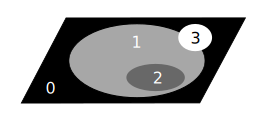
\includegraphics[trim= 0mm 0mm 0mm 5mm, clip, scale=0.75]{Formulation/figure/abc_img.pdf}}		    \hspace{0cm}
		    %\subfloat[$G_T=(S,A_T)$\label{fig:abc_graph_topo}]{
\includegraphics[scale=0.8]{Formulation/figure/abc_graph_topo.pdf}}	
		    \subfloat[Graphe $G_T$\label{fig:abc_graph_topo}]{
\includegraphics[trim= -10mm 0mm -10mm 0mm, clip, scale=0.8]{Formulation/figure/abc_graph_topo.pdf}}	\hspace{0cm}
		    %\subfloat[$G_P=(S,A_P)$\label{fig:abc_graph_photo}]{
\includegraphics[scale=0.8]{Formulation/figure/abc_graph_photo.pdf}}	
		    \subfloat[Graphe $G_P$\label{fig:abc_graph_photo}]{
\includegraphics[trim= -10mm 0mm -10mm 0mm, clip, scale=0.8]{Formulation/figure/abc_graph_photo.pdf}}	\hspace{0cm}
		     \subfloat[Gradien $G_P$\label{fig:abc_graph_photo_gradient}]{\includegraphics[trim= 0mm 0mm 0mm 0mm, clip, scale=0.5]{Formulation/figure/abc_graph_photo_gradient.pdf}}
		}\caption{ Exemple d'une image et des graphes conceptuels associés.}
         \label{fig:img_and_graph}
	\end{figure}
	%%%%%%%%%%%%%%%%%%%%%%%%%%%%%%%%%%%%%%%%%%%%%%%%%%%

	Selon l'image~\ref{fig:abc_img}, l'ensemble $S$ est égal à $\{0,1,2,3\}$. Sur le graphe~\ref{fig:abc_graph_topo} on représente les inclusions partielles et totales des régions. On voit que la région 2 est complètement incluse dans 1, qui est elle même incluse dans 0. La régions 3 quand à elle est incluse partiellement dans 1 et 2. Cette information se traduit par deux arcs entrant sur le n\oe{}ud 3 (fig.~\ref{fig:abc_graph_topo}). Dans le second graphe (fig.~\ref{fig:abc_graph_photo}), on représente les relations d'intensité lumineuse caractérisées par des arcs entrants (plus clair que) et sortant (plus sombre que). On retrouve par lecture du graphe, que 0 est la région la plus sombre (aucun arc entrant) et 3 la plus claire (aucun arc sortant). 
	
	La disposition spatiale des n\oe{}uds est identique pour les deux graphes pour souligner leurs différences limitées aux arcs qui les composent. Une autre représentation équivalente des informations photométriques peut être la figure~\ref{fig:abc_graph_photo_gradient} où l'on positionne les étiquettes des régions selon un gradient de niveaux de gris.

	%Note\footnote{la représentation en ligne de 1.1c) et plus simple à comprendre que celle sur la base de la structure topologique, mais cette dernière sera plus simple à implémenter si on combine les deux graphes. Que choisir? {\bf: cf propositions: la distribution spatiale des noeuds est la même dans les deux, permettant ainsi de souligner la différence entre info topo et photo.}}\\
	Par la suite, selon si les arcs traduisent une information topologique ou photométrique, nous aurons deux types de graphes, respectivement symbolisés par $G_T$ (fig.~\ref{fig:abc_graph_topo}) et $G_P$ (fig.~\ref{fig:abc_graph_photo} ), reposant sur les mêmes n\oe{}uds mais se distinguant selon les arcs :
	\begin{itemize}
		\item
		Topologique: $G_T=(S, A_T)$ %(actuellement: $F=G$, sans écrire mathématiquement que $F$ est un graphe associé à un ensemble de sommets ($S$) et d'arêtes (pas de notation)). 
		\item
		Photométrique: $G_P=(S,A_P)$
	\end{itemize}

	 Où $S$ est l'ensemble des n\oe{}uds (types) et $A_x$ l'ensemble des arcs les reliant.
	 
	Nous nous appuierons sur le formalisme de \citep[Fasquel]{Fasquel2006} en changeant quelques notations de sorte à rester cohérent avec notre étude. En effet dans son travail, il n'y avait pas de distinction de type d'arc car seule l'information topologique était considérée. L'intégration de la photométrie nécessite donc d'affiner les notations. On remplace $F$ par $G_T$ (pour graphe topologique), on utilise les notions de ``prédécesseurs/successeurs'' au lieu de ``pères/fils'' et on change l'orientation des arcs du graphe topologique. %pour être cohérent avec la \textbf{théorie des graphes [REF]}.


\subsection{Relations: illustration dans le cas topologique}

	Pour tous les éléments $i$ contenu dans l'ensemble $S$, $G_T^{+1}(i)$ est un sous ensemble de $S$ qui contient les ``successeurs''  directs (à une distance de +1) de $i$, $G_T^{-1}(i)$ ses prédécesseurs directs. Notons $G_T^{-1}(0) = \emptyset$ et $\forall i \in S,\; G_T(i) \subseteq S$. Une autre notation $G_{T}^{-\infty}(i)$, représente tous les ``prédécesseurs'' (jusqu'à la racine du graphe) d'un type $i$, par exemple, sur la figure~\ref{fig:a_priori_info},  $G_{T}^{-\infty}(4)=\{2,0\}$.


	%%%%%%%%%%%%%%%%%%%%%%%%%%%%%%%%%%%%%%%%%%%%%%%%%%%
	\begin{figure}[!ht]	%trim=l b r t
	  \centering
	      \fbox{
		  \subfloat[Graphe $(G_T)$]{\label{fig:a_priori_topo_graph}
\includegraphics[trim= 0mm 5mm 0mm 5mm, clip, scale=0.3]{Formulation/figure/info_topo_graph.pdf}}
		  \subfloat[Image à priori $(I)$]{\label{fig:a_priori_topo_img}\includegraphics[trim= 0mm 20mm 0mm 15mm, clip, scale=0.4]{Formulation/figure/a_priori_img.pdf}}

		  %\fbox{\includegraphics[trim= 0mm 30mm 0mm 15mm, clip, scale=0.3]{Formulation/figure/info_topo.pdf}}	%trim=l b r t  width=0.5\textwidth, 

		  %\includegraphics[width=0.5\textwidth]{Formulation/figure/info_topo.pdf}
		}\caption{Exemple de représentation d'informations topologiques à priori.}
         \label{fig:a_priori_info}
	\end{figure}
	%%%%%%%%%%%%%%%%%%%%%%%%%%%%%%%%%%%%%%%%%%%%%%%%%%%

	Le graphe~\ref{fig:a_priori_topo_graph} représente un ensemble $S$ = \{0, 1, 2, 3, 4, 5, 6\} ayant des relations topologiques particulières définies par les arcs $A_T$, associées à une notion de recouvrement total ou partiel. On peut aisément déterminer les régions contenues (même partiellement) dans une région donnée en utilisant la notion de ``prédécesseurs'' : $G_T^{-1}(0)=\emptyset$, $G_T^{-1}(1) = \{0\}$, $G_T^{-1}(2) = \{0\}$, $G_T^{-1}(3) = \{2\}$, $G_T^{-1}(4) = \{2\}$, $G_T^{-1}(5) = \{2,4\}$, $G_T^{-1}(6) = \{4\}$. 

	Ou inversement, en utilisant la notion de ``successeurs'' : $G_T^{1}(0)=\{1,2\}$, $G_T^{1}(1) = \emptyset$, $G_T^{1}(2)=\{3,4,5\}$, $G_T^{1}(3)=\emptyset$, $G_T^{1}(4)=\{5,6\}$, $G_T^{1}(5)=\emptyset$, $G_T^{1}(6)=\emptyset$.

	Les informations à priori dépendent donc d'un ensemble de types $(S)$ qui ont des propriétés d'inclusion (arcs $A_T$ dans $G_T$), et de l'image $(I)$. On les note $C=\{G_T, I\}$.\vspace{1em}

	En considérant l'imagerie médicale comme domaine d'application, on peut associer les éléments de $S$ à des structures anatomiques (e.g. foie, rate) ou pathologiques (e.g. tumeur hépatique), ou bien à des structures relatives au système d'imagerie (e.g. table sur laquelle le patient est placé lors de l'acquisition de l'image). Ainsi, on pourrait par exemple assimiler ces régions à l'acquisition (0), la table sur laquelle est placée le patient dans l'imageur (1), le corps (2), la rate (3), le foie (4), un vaisseau hépatique (5) et une tumeur du foie (6). $G_T^{-1}(5)=\{4,2\}$ signifierait donc que le vaisseau hépatique est contenu par la région du foie et du corps mais pas par celle de la rate par exemple. 


      %{\bf Attention notation: $\mathbf{S}=\{0, ..., N\}$ puis (après) $S$ = \{A,B,C,D,E,F,G\}: rester homogène et ne considérer qu'une seule notation: soit 0..N, soit A..X : alternative privilégier 0...N (plus simple de manipuler des numéros que des lettres). On pourra éventuellement utiliser $S=\{L_0, ..., L_N\}$, ou $S=\{L_i \}$ avec $i=\{0,...,N\}$ L: étiquette associée à une région (Label en anglais).}

    \section{Intégration du processus d'analyse séquentiel}
	Dans le cadre d'un processus d'analyse séquentiel, il s'agit d'intégrer l'information relative aux régions déjà segmentées : les étapes de segmentation suivantes prennent alors en compte le contexte, à savoir les informations (contextuelles) sur les régions déjà identifiées \citep[Fasquel]{Fasquel2006}. Les informations contextuelles se distinguent des précédentes par un indice de temps qui s'apparente aux itérations. On les notera $C_t=\{G_{T,t}, I_t\}$ avec $G_{T,t}=(S_t,A_T)$.\\
	$G_{T,t}$ est équivalent à $G_T$ dans lequel seulement certains n\oe{}uds $u\in S_t$ sont valides (correspondant à des régions déjà segmentées, même partiellement). Pour pouvoir différencier visuellement, nous intégrerons la notion d'activation de noeud du graphe conceptuel initial, comme considéré récemment par \citep[Fasquel]{Fasquel2006} (voir fig.~\ref{fig:info_topo_context_graph}). Dans le même esprit, nous encadrerons en noir le type recherché. L'ensemble $S_t \subseteq S$ comprends tous les types de régions qui ont été segmentés jusqu'à $t-1$. A $t=0$, lors de la première séquence, on a $S_0=\{0\}$ car toute l'image est implicitement identifiée. Les arêtes de $G_{T,t}$ demeurent inchangées et correspondent à $A_T$.\\
	$\forall u \in S$, $G_{T,t}^{-1}(u)$ renvoie les prédécesseurs valides à $t$. Par exemple, dans la figure~\ref{fig:info_topo_context_graph}, où seul 1 et 4 ne sont pas valides, les prédécesseurs valides de 5 à $t$ sont définit par $G_{T,t}^{-1}(5)=\{2\}$.\\
	Tout comme $I$, $I_t = \{X_t(u)\;|\;u \in S_t\}$ (fig.~\ref{fig:topo_img}), où $X_t(u)$ est la région d'une structure $u$ déjà segmentée ($u \in S_t \Leftrightarrow X_t(u) \neq \emptyset$).


	%%%%%%%%%%%%%%%%%%%%%%%%%%%%%%%%%%%%%%%%%%%%%%%%%%%
	\begin{figure}[!ht]	%trim=l b r t  width=0.5\textwidth, 
	  \centering
	      \fbox{
		  \subfloat[Graphe ($G_{T,t}$)]{\label{fig:info_topo_context_graph}\includegraphics[trim= 0mm 5mm 0mm 0mm, clip, scale=0.3]{Formulation/figure/info_topo_context_graph.pdf}}
		  \subfloat[Image($I_t$)]{\label{fig:topo_img}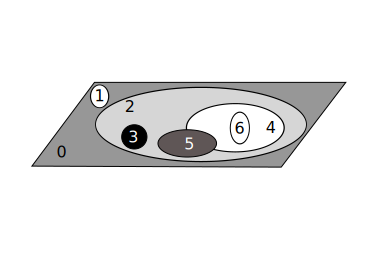
\includegraphics[trim= 0mm 15mm 0mm 10mm, clip, scale=0.47]{Formulation/figure/info_topo_context_image.pdf}}
		  \subfloat[Région de $R_t(5)$]{\label{fig:info_topo_context_image_ex}\includegraphics[trim= 0mm 18mm 0mm 10mm, clip, scale=0.5]{Formulation/figure/info_topo_context_image_ex.pdf}}
	      }\caption{Exemple d'information contextuelles à $t$. Les n\oe{}uds en gris sont dit invalidés, à l'inverse de ceux en noir qui sont valides. En faisant l'analogie avec la figure~\ref{fig:a_priori_info}, la table (1) et le foie (4) ne sont pas segmentés à cette date $t$. }
         \label{fig:contextual_info}
	\end{figure}
	%%%%%%%%%%%%%%%%%%%%%%%%%%%%%%%%%%%%%%%%%%%%%%%%%%%

\newpage
     \section{Inférence et topologie: région d'intérêt}

	On propose de reprendre la définition de la région d'intérêt (Region Of Interest) proposée par \citep[Fasquel]{Fasquel2006} qui défini la ROI optimale d'un type $u \in S$ comme :

	%%%%%%%%%%%%%%%%%%%%%%%%%%%%%%%%%%%%%%%%%%%%%%%%%%%
	\begin{equation}
		R_t(u)=\left(\bigcup_{l\in G_{T,t}^{-1}(u)}X_t(\overline{l})\right) \cup \left(\bigcup_{i\in S_t| u\in G_{T,t}^{-\infty}(i)}X_t(i) \right)
		\label{eq:roi}
	\end{equation}
	%%%%%%%%%%%%%%%%%%%%%%%%%%%%%%%%%%%%%%%%%%%%%%%%%%%

% 	\begin{center}
% 		\begin{tabular}{ll}
% 		$t$ 		& : numéro (date) d'une itération \\
% 		$u$ 		& : type recherché (cible) \\
% 		$i$		& : type générique appartenant à l'ensemble $S$ \\
% 		$l$ 		& : élément (liaison) du sous ensemble $F_t$ \textbf{???}\\
% 		            & {\bf élément de l'ensemble des prédécesseurs (dans $S_t$)}:\\
% 				 & {\bf étiquette d'une des régions déjà segmentées contenant (au moins partiellement) $u$}\\
% 		$\bar{l}$	& : \textbf{???} \\
% 		$R_t(u)$ 	& : ROI optimale au sens [Fasquel] d'un type $u$ \\
% 		$F_t(u)$ 	& : les informations inter-régions (inter-n\oe{}uds) à $t$ qui concernent la cible $u$ \\
% 		$X_t(\bar{l})$ 	& : région d'une structure $\bar{l}$ déjà segmentée \textbf{???} {\bf (voir ci-dessous)}\\
% 		$X_t(i)$ 	& : région d'une structure $i$ déjà segmentée \\
%  		$F^\infty(i)$ 	& : ensemble des ancêtres de l'élément $i$ (jusqu'au ``root'') \\
% 		$S_t$ 		& : ensemble des types de régions qui ont étaient segmentés entre $t$ et $t-1$ \\
% 		\end{tabular}
% 	\end{center}	 
% 
% {\bf $\bar{l}$: résidu vs l (voir article pour définition). En terme d'images, cela correspond à ce qui reste d'une région quand on a enlevé toutes les régions (dont les étiquettes sont les prédécesseurs de $l$ dans le graphe) qu'elle peut contenir: ce reste est une région dont le labele/étiquette/identité est $\bar{l}$. Cette étiquette correspond à un noeud implicite du graphe.}

	Le premier membre correspond à l'union des prédécesseurs directs de la cible. La région est réduite autour de la cible par les informations contextuelles des relations, symbolisées par $G_{T,t}$. En fait, cette réduction est réalisée par suppression des régions déjà segmentées qui intersectent les régions supposées contenir la cible (au moins partiellement). Ces structures peuvent être du même type que la cible recherchée mais on suppose que deux structures du même type ne s'intersectent pas.

	Le second terme vérifie que les régions qui recouvrent partiellement la cible soit conservées dans la ROI. Cela permet par exemple de ne pas supprimer une partie du foie qui serai recouverte par le vaisseau hépatique en supprimant le vaisseau hépatique.

	Prenons par exemple, une cible de type $6$ (tumeur du foie) :

	%%%%%%%%%%%%%%%%%%%%%%%%%%%%%%%%%%%%%%%%%%%%%%%%%%%
	\begin{equation}
		R_t(6)=\left(\bigcup_{l\in G_{T,t}^{-1}(6)}X_t(\overline{l})\right) \cup \left(\bigcup_{i\in S_t| 6\in G_{T,t}^{-\infty}(i)}X_t(i) \right)
		\label{eq:roi_ex}
	\end{equation}
	%%%%%%%%%%%%%%%%%%%%%%%%%%%%%%%%%%%%%%%%%%%%%%%%%%%

	De part les informations contextuelles rappelées sur la figure~\ref{fig:info_topo_context_graph}, on a $\{l \in G_{T,t}^{-1}(6)\} = G_{T,t}^{-1}(6) = \{2\}$ et $\{i \in S_t \;|\;6\in G_{T,t}^{-\infty}(i) \}=\emptyset$ ce qui nous amène à $R_t(6)=X_t(2) \setminus (X_t(3) \cup X_t(5) \cup X_t(6))$ . On  représente cette région en blanc sur la figure~\ref{fig:info_topo_context_image_ex}.


	%%%%%%%%%%%%%%%%%%%%%%%%%%%%%%%%%%%%%%%%%%%%%%%%%%%
% 	\begin{figure}[!ht]	% ! here top bottom
% 	  \centering
% 	      \fbox{
% 		  \subfloat[Graphe ($G_{T,t}$)]
% 		  {\label{fig:info_topo_context_graph_ex}
\includegraphics[trim= 0mm 5mm 0mm 5mm, clip, scale=0.3]{Formulation/figure/info_topo_context_graph_ex.pdf}}	%trim=l b r t
% 		  \subfloat[Région de $R_t(6)$]{\label{fig:info_topo_context_image_ex}\includegraphics[trim= 0mm 20mm 0mm 15mm, clip, scale=0.5]{Formulation/figure/info_topo_context_image_ex.pdf}}	%trim=l b r t  width=0.5\textwidth, 
% 	      }\caption{Graphe d'informations contextuelles. {\bf tu devrais faire une seule figure avec \ref{fig:contextual_info}: sous-figure (b) de \ref{fig:contextual_info_rappel_ex} devient (c) dans fig. \ref{fig:contextual_info}}}
%          \label{fig:contextual_info_rappel_ex}
% 	\end{figure}
	%%%%%%%%%%%%%%%%%%%%%%%%%%%%%%%%%%%%%%%%%%%%%%%%%%%


% \newpage
%       \subsubsection{Nombre de classes}
% 
% 	Nous définissons le nombre de classes par la cardinalité de l'ensemble des n\oe{}uds non segmentés (ensemble des n\oe{}uds moins les n\oe{}uds déjà segmentés) appartenant à la ROI. Ici nous considérons toutes les classes possibles en omettant l'aspect optionnel des types pathologiques. Ce nombre est définit par la formule suivante :
% 
% 	%%%%%%%%%%%%%%%%%%%%%%%%%%%%%%%%%%%%%%%%%%%%%%%%%%%
% 	\begin{equation}
% 		%N_t(u) = \operatorname{Card}\{X_t(i) \in R_t(u) \; \forall \;i\}
% 		N_t(u) = \operatorname{Card}\{i \in S \setminus S_t \;|\; X(i) \in R_t(u)\}
% 		%nbClMax = \operatorname{Card}\{R_t(u)\}
% 		\label{eq:nb_classe}
% 	\end{equation}
% 	%%%%%%%%%%%%%%%%%%%%%%%%%%%%%%%%%%%%%%%%%%%%%%%%%%%
% 
% 	\begin{center}
% 		\begin{tabular}{ll}
% 		$u$ 	& : n\oe{}ud correspondant à un type de structure (cible) \\
% 		$i$	& : élément (intersection) de l'ensemble $S$ \\
% 		$N_t(u)$& : nombre de classes attendue pour le n\oe{}ud $u$ \\
% 		$R_t(u)$& : ROI en fonction d'une structure cible $u$ \\
% 		$X(i)$	& : région d'une structure cible $i$ issue de l'ensemble de structures $S$ au temps $t$\\
% 		$S_t$ 	& : ensemble des types de régions qui ont étaient segmentés entre $t$ et $t-1$ \\
% 		$S$ 	& : ensemble des structures à priori \\
% 		\end{tabular}
% 	\end{center}
% 
% 	%%%%%%%%%%%%%%%%%%%%%%%%%%%%%%%%%%%%%%%%%%%%%%%%%%%
% 	\begin{figure}[!ht]
% 	  \centering
% 	      \subfloat[Graphe]{\label{fig:info_topo_nb_class}\includegraphics[trim= 0mm 5mm 0mm 5mm, clip, scale=0.3]{Formulation/figure/info_topo_context_graph.pdf}}	%trim=l b r t  width=0.5\textwidth, 
% 		\subfloat[Image]{\label{fig:topo_img}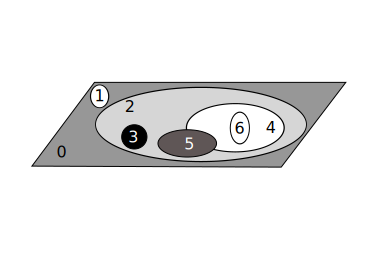
\includegraphics[trim= 0mm 30mm 0mm 15mm, clip, scale=0.4]{Formulation/figure/info_topo_context_image.pdf}}	%trim=l b r t 
% 	      \caption{Exemple de recherche du nombre de classes. }
%          \label{fig:contextual_info}
% 	\end{figure}
% 	%%%%%%%%%%%%%%%%%%%%%%%%%%%%%%%%%%%%%%%%%%%%%%%%%%%
%\newpage
    \section{Inférence et photométrie}
    \label{sec:inf_and_photo}
	Les déductions faites à partir des connaissances disponibles à $t$ par le moteur d'inférence\footnote{Moteur d'inférence : de l'anglais ``enference engine'' et du verbe ``inférer'' qui signifie ``déduire'', c'est un concept de raisonnement déductif à qui on demande des informations et qui déduit des conclusions à partir d'une base de faits et d'une base de connaissances.}, portent sur les propriétés photométriques de la région au sein de laquelle vont s'effectuer les traitements. 

Ces propriétés photométriques que l'on propose d'inférer, concernent le nombre de classes ``photométriques'' de la ROI ainsi que leurs relations d'ordres, permettant ainsi d'associer une classe à un noeud du graphe, c'est à dire à une région bien identifiée. Il est à noter que ces déductions dépendent de celles considérées dans la section précédente au sujet de la région d'intérêt optimale.

Pour cette première phase de l'étude, nous faisons l'hypothèse simplificatrice que toutes les régions ont une multiplicité de 1. Cela signifie qu'elles sont dans l'image (aucune n'est optionnelle) et qu'elles sont uniques, il ne peut donc pas y avoir deux tumeurs hépatiques par exemple.

      \subsection{Nombre de classes}
	%Ici nous considérons tous les types possibles en omettant l'aspect optionnel ou multiple des types pathologiques. Une multiplicité de un, signifie que chaque type est unique dans l'image, il ne peut donc pas y avoir deux tumeurs hépatiques par exemple. 
	L'objectif est d'isoler un sous-ensemble à priori de types correspondant aux lobes issues d'une région d'intérêt dans l'histogramme d'une image. On présente ci-dessous les étapes majeures qui ont contribué à l'établissement de la formule finale.

	Dans un premier temps, nous utilisons la notion de ``ROI optimale'' présentée dans la section précédente pour déterminer un sous-ensemble nommé $L_t(u)$. Ce sous-ensemble est composé de l'ensemble des types non segmentés ($S \setminus S_t$) inclus dans la région d'intérêt d'un type $u$ et de ses prédécesseurs directs ($G_{T,t}^{-1}(u)$). Formule initiale :

	%%%%%%%%%%%%%%%%%%%%%%%%%%%%%%%%%%%%%%%%%%%%%%%%
	\begin{equation}
		%N_t(u) = \operatorname{Card}\{X_t(i) \in R_t(u) \; \forall \;i\}
		L_t(u) = \{i \in S \setminus S_t \;|\; X(i) \in R_t(u)\} \cup G_{T,t}^{-1}(u)
		%L_t(u) = \{i \in S \setminus S_t \;|\; X(i) \in R_t(u) \; AND \; G_{P,t}^{[u,iMin]} \}
		%nbClMax = \operatorname{Card}\{R_t(u)\}
		\label{eq:nb_lobe}
	\end{equation}
	%%%%%%%%%%%%%%%%%%%%%%%%%%%%%%%%%%%%%%%%%%%%%%%%

	Durant l'expérimentation de cette formule, nous nous sommes demandé si l'on pouvait la simplifier du fait que la région $R_t(u)$ et les successeurs $G_{T,t}^{-1}(u)$ utilisaient les mêmes informations à priori. En effet la région peut être exprimée par l'ensemble des successeurs des prédécesseurs de $u$ : $G_T^{\infty}(G_{T,t}^{-1}(u))$.	La formule précédente devient :

	%%%%%%%%%%%%%%%%%%%%%%%%%%%%%%%%%%%%%%%%%%%%%%%%
	\begin{equation}
	L_t(u) =  \{ i\in S \setminus S_t|\; i \in G_T^{\infty}(G_{T,t}^{-1}(u))\} \cup G_{T,t}^{-1}(u)
	\end{equation}
	%%%%%%%%%%%%%%%%%%%%%%%%%%%%%%%%%%%%%%%%%%%%%%%%

	Elle peut se simplifier en remplaçant le premier membre par l'intersection de l'ensemble non segmenté avec l'ensemble des successeurs des prédécesseurs : 

%remplaçant l'union de l'ensemble de ses successeurs non segmentés d'un type de $\{ i\in S \setminus S_t|\; i \in G_T^{\infty}(i)\}$ par $G_T^{\infty}(k) \cap \{S \setminus S_t\}$. :

	%%%%%%%%%%%%%%%%%%%%%%%%%%%%%%%%%%%%%%%%%%%%%%%%
	\begin{equation}
		L_t(u) = \left\{ ( S \setminus S_t ) \cap  G_T^{\infty}(G_{T,t}^{-1}(u)) \right\} \cup G_{T,t}^{-1}(u)
	\end{equation}
	%%%%%%%%%%%%%%%%%%%%%%%%%%%%%%%%%%%%%%%%%%%%%%%%

	Une forme plus généraliste de $L_t(u)$ pourrait être, pour un élément $i$ issu des prédécesseurs de $u$ ($i\in G_{T,t}^{-1}(u)$), l'union de l'ensemble des successeurs non segmentés dont les prédécesseurs actifs font parti de $G_{T,t}^{-1}(u)$ et des prédécesseurs de $u$ eux-mêmes ($G_{T,t}^{-1}(u)$). 

	%%%%%%%%%%%%%%%%%%%%%%%%%%%%%%%%%%%%%%%%%%%%%%%%
	\begin{equation}
		L_t(u) =  \left(\bigcup_{i\in G_{T,t}^{-1}(u)} ( S \setminus S_t ) \cap G_T^{\infty}(i) \right) \cup G_{T,t}^{-1}(u) 
	\end{equation}
	%%%%%%%%%%%%%%%%%%%%%%%%%%%%%%%%%%%%%%%%%%%%%%%%

	Nous avons pu constater lors de tests, une faiblesse de cette formule dans des cas limites comme lorsque l'origine du graphe (0) fait parti des prédécesseurs de $u$ ou encore quand $u$ a plusieurs prédécesseurs actifs.% lorsque la racine du graphe $G_t(0)$ faisait partie de l'ensemble $G_{T,t}^{-1}(u)$. Dans ce cas, $G_T^{\infty}(G_{T,t}^{-1}(u))$ est égal à l'ensemble des n\oe{}uds de $S$ ce qui fausse le résultat puisque qu'il contient des types non actif successeurs de types actifs. Nous devons donc les soustraire : $G_T^{\infty}(G_{T,t}^{-1}(u)) \setminus G_T^{\infty} (G_{T,t}^{+1}(G_{T,t}^{-1}(u)) )$. Dans la formule suivante on notera l'ensemble des successeurs valides $G_{T,t}^{-1}(u)=U$ pour alléger les notations.


	%%%%%%%%%%%%%%%%%%%%%%%%%%%%%%%%%%%%%%%%%%%%%%%%
% 	\begin{equation}
% 	      L_t(u) = \left\{ ( S \setminus S_t ) \cap ( G_T^{\infty}(U) \setminus G_T^{\infty} (G_{T,t}^{+1}(U) ) ) \right\} \cup U 
% 	\end{equation}
	%%%%%%%%%%%%%%%%%%%%%%%%%%%%%%%%%%%%%%%%%%%%%%%%
	
% 	Simplification proposée :
% 
% 	%%%%%%%%%%%%%%%%%%%%%%%%%%%%%%%%%%%%%%%%%%%%%%%%%%%
% 	\begin{equation}
% 	  %L_t(5) = & \left( ( S \setminus S_t ) \cap G_{T}^\infty \left( G_T^{-1}(5) \setminus G_{T,t}^{-1} \left( 5 \right) \right) \right) \cup G_{T,t}^{-1}(5) \\
% 	 L_t(u) = \left( ( S \setminus S_t ) \cap \left( G_T^{+1}(i) \;|\; i \in G_{T,t}^{-1}(u) \right) \right) \cup G_{T,t}^{-1}(u)
% 	\end{equation}
	%%%%%%%%%%%%%%%%%%%%%%%%%%%%%%%%%%%%%%%%%%%%%%%%%%%

	Nous proposons donc la formule suivante qui renvoie l'ensemble des types qui succèdent aux prédécesseurs de $u$ ($G_T^{\infty}(G_{T,t}^{-1} (u))$), non actifs, ($\cap\; S \setminus S_t$), et qui ont au moins un prédécesseur actif direct en commun avec $u$ ($G_{T,t}^{-1} (i) \cap G_{T,t}^{-1} (u) \neq \emptyset$). A cet ensemble on ajoute l'ensemble des prédécesseurs de $u$ avec $G_{T,t}^{-1}(u)$ :
	%%%%%%%%%%%%%%%%%%%%%%%%%%%%%%%%%%%%%%%%%%%%%%%%%%%
	\begin{equation}
 	  L_t(u) = \left\{ i \in \left( G_T^{\infty}(G_{T,t}^{-1} (u)) \cap ( S \setminus S_t ) \right) \;|\; \left( G_{T,t}^{-1} (i) \cap G_{T,t}^{-1} (u) \neq \emptyset \right) \right\} \cup  G_{T,t}^{-1}(u)\\
	\end{equation}
	%%%%%%%%%%%%%%%%%%%%%%%%%%%%%%%%%%%%%%%%%%%%%%%%%%%


	De cette relation, nous pouvons à présent compter le nombre de lobes $N_t$ attendus dans l'image à $t$ par la cardinalité (nombre d'éléments) du sous-ensemble $L_t(u)$ : $ N_t(u) = \left|{L_t(u)}\right|$. Rappelons que le nombre de lobes à priori est calculé pour optimiser le paramétrage d'algorithmes de segmentation.
	
		\subsubsection*{Exemples applicatifs}
	Application à une image, qui a les propriétés topologiques $G_{T,t}$, dans laquelle on cherche toutes les lobes à priori pour une ROI dans le but de les dénombrer puis de les identifier. On fera un aperçu du résultat graphique sur l'histogramme représentatif d'une image, dans lequel nous ferons apparaître les lobes correspondant aux types segmentés en trait plein. Les lobes en trait discontinu sont considérées comme inconnues. La position des lobes dans l'histogramme et leurs niveaux de gris (en abscisse de l'histogramme) sont représentés selon les informations photométriques à priori issue du graphe $G_P$ associé. Ce dernier ne sera utilisé qu'à titre d'illustration dans cette section (aucune utilisation de son information).\vspace{1em}

\begin{itemize}
\item Cas 1 : recherche du type $1$ sachant que les types $0$ et $2$ ont été segmentés :
\end{itemize}

	%%%%%%%%%%%%%%%%%%%%%%%%%%%%%%%%%%%%%%%%%%%%%%%%%%%
	\begin{figure}[!ht]	%trim=l b r t  width=0.5\textwidth,
	  \centering
	      \fbox{
		  \subfloat[Graphe $G_{T,t}$]{\label{fig:cas_1_graph_topo}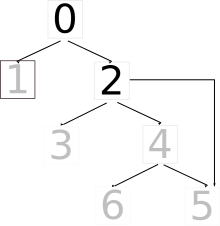
\includegraphics[trim= -10mm 0mm -10mm 0mm, clip, scale=0.4]{Formulation/figure/cas_1_graph_topo.pdf}}
		  %\subfloat[Région $R_t(1)$]{\label{fig:cas_1_img}\includegraphics[trim= 8mm 5mm 10mm 5mm, clip, scale=0.5]{Formulation/figure/cas_1_img.pdf}}
		  \subfloat[Histogramme]{\label{fig:cas_1_histo}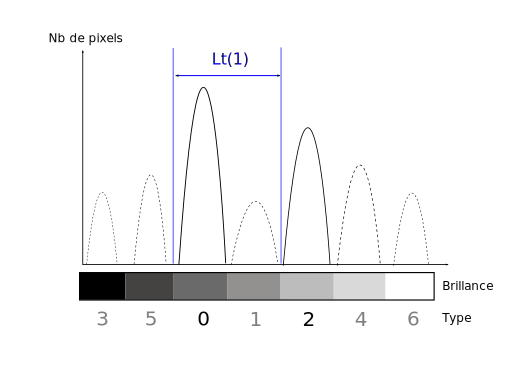
\includegraphics[trim= 0mm 10mm 0mm 5mm, clip, scale=0.4]{Formulation/figure/cas_1_histo.pdf}}
		  \subfloat[Graphe $G_{P,t}$]{\label{fig:cas_1_graph_photo}
\includegraphics[trim= -10mm -5mm -10mm 0mm, clip, scale=0.4]{Formulation/figure/cas_1_graph_photo.pdf}}
	      }\caption{Sous-ensemble $L_t(1)$.}
	  \label{fig:cas_1}
	\end{figure}
	%%%%%%%%%%%%%%%%%%%%%%%%%%%%%%%%%%%%%%%%%%%%%%%%%%%


	%%%%%%%%%%%%%%%%%%%%%%%%%%%%%%%%%%%%%%%%%%%%%%%%%%%
	\begin{equation}
	 \begin{split}
	  L_t(1) = & \left\{ i \in \left( G_T^{\infty}(G_{T,t}^{-1}(1)) \cap ( S \setminus S_t ) \right) \;|\; \left( G_{T,t}^{-1} (i) \cap G_{T,t}^{-1} (1) \neq \emptyset \right) \right\} \cup  G_{T,t}^{-1}(1)\\
		 = & \left\{ i \in \left( \{1,2,3,4,6,5\} \cap \{1,3,4,6,5\} \right) \;|\; \left( G_{T,t}^{-1} (i) \cap \{0\} \neq \emptyset \right) \right\} \cup  \{0\}\\
		 = & \left\{1 \right\} \cup  \{0\}\\
	 \end{split}
	 \label{eq:cas1}
	\end{equation}
	%%%%%%%%%%%%%%%%%%%%%%%%%%%%%%%%%%%%%%%%%%%%%%%%%%%

	Le type 2 étant segmenté, il est exclu du sous-ensemble ($S \setminus S_t$) ainsi que les types 3, 4, 5 et 6 car ils n'ont pas de prédécesseurs direct en commun avec ceux de 1 $\left( G_{T,t}^{-1} (i) \cap G_{T,t}^{-1} (u) \neq \emptyset \right)$. Selon le graphe topologique figure~\ref{fig:cas_1_graph_topo}. Le deuxième membre $G_{T,t}^{-1}(1) = \{0\}$ car 1 n'a que 0 comme prédécesseur valide, il en résulte un ensemble de types $L_t(1) =  \{1, 0\}$. Cet ensemble est représenté sur la figure~\ref{fig:cas_1_histo} selon $G_{P}$ (fig.~\ref{fig:cas_1_graph_photo}). Sa cardinalité $N_t(1)=\left|{L_t(1)}\right| = 2$.\vspace{1em}
	
\begin{itemize}
\item 	Cas 2 : recherche du type $3$ sachant que les types 0, 1 et 2 ont été segmentés :
\end{itemize}

	%%%%%%%%%%%%%%%%%%%%%%%%%%%%%%%%%%%%%%%%%%%%%%%%%%%
	\begin{figure}[!ht]	%trim=l b r t  
	  \centering
	      \fbox{		  
		  \subfloat[Graphe $G_{T,t}$]{\label{fig:cas_2_graph_topo}\includegraphics[trim= 20mm 0mm 0mm 5mm, clip, scale=0.4]{Formulation/figure/cas_2_graph_topo.pdf}}
		  \subfloat[Histogramme]{\label{fig:cas_2_histo}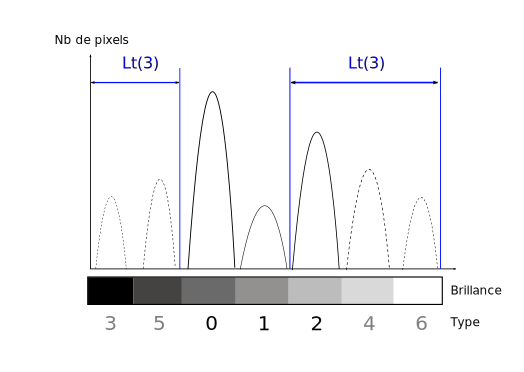
\includegraphics[trim= 0mm 10mm 0mm 5mm, clip, scale=0.4]{Formulation/figure/cas_2_histo.pdf}}
		  \subfloat[Graphe $G_{P,t}$]{\label{fig:cas_2_graph_photo}
\includegraphics[trim= -10mm -5mm -10mm 0mm, clip, scale=0.4]{Formulation/figure/cas_2_graph_photo.pdf}}
	      }\caption{Sous-ensemble $L_t(3)$.}
         \label{fig:cas_2}
	\end{figure}
	%%%%%%%%%%%%%%%%%%%%%%%%%%%%%%%%%%%%%%%%%%%%%%%%%%%

	%%%%%%%%%%%%%%%%%%%%%%%%%%%%%%%%%%%%%%%%%%%%%%%%%%%
	\begin{equation}
	 \begin{split}
	  L_t(3) = & \left\{ i \in \left( G_T^{\infty}(G_{T,t}^{-1}(3)) \cap ( S \setminus S_t ) \right)\;|\; \left( G_{T,t}^{-1} (i) \cap G_{T,t}^{-1} (3) \neq \emptyset \right) \right\} \cup  G_{T,t}^{-1}(3)\\
		 = & \left\{ i \in \left( G_T^{\infty}(\{2\}) 		\cap \{3,4,6,5\} 	 \right)\;|\; \left( G_{T,t}^{-1} (i) \cap \{2\} \neq \emptyset \right) \right\} \cup \{2\} \\
		 = & \left\{ 3,4,6,5 \right\} \cup \left\{ 2 \right\} \\
	 \end{split}
	 \label{eq:cas2}
	\end{equation}
	%%%%%%%%%%%%%%%%%%%%%%%%%%%%%%%%%%%%%%%%%%%%%%%%%%%

	Ici l'ensemble des types non segmentés $S \setminus S_t = \{3,4,5,6\}$ sont conservés car ils ont tous le même prédécesseur (fig.~\ref{fig:cas_2_graph_topo}). Le deuxième membre $G_{T,t}^{-1}(3) = \{2\}$ (seul prédécesseur valide de 3), il en résulte un ensemble de types $L_t(3) = \{3,4,6,5,2\}$. Cet ensemble est représenté sur l'histogramme~\ref{fig:cas_2_histo}. Sa cardinalité $N_t(3) = \left|{L_t(3)}\right| = 5$.\vspace{1em}

  %En revanche, de part les relations photométriques (fig.~\ref{fig:cas_2_graph_photo}) seul les types 3 et 5 sont conservés puisque 4 et 6 sont plus brillants que les types segmentés (régions connues). Il en résulte un ensemble de lobes $L_t(3) =  \{5,3\}$. 
%{\bf A mon avis, si l'on cherche 3, la ROI est en effet restreinte à $X_t(2)$, et il y aura 5 lobes, sans même regarder la formule: $L_t(3) =  \{2,3,4,5,6\}$, $2$ correspondant au fond de la ROI. Si on applique la formule suivante: $L_t(u) = \{i \in S \setminus S_t \;|\; X(i) \in R_t(u)\} \cup \{ G_{T,t}^{-1}(u) \}$:

% \begin{itemize}
% \item
% $\{i \in S \setminus S_t \;|\; X(i) \in R_t(3)\} = \{3,4,5,6\}$
% \item
% $\{ G_{P,t}^{-1}(3) \} = \{2\}$
% \end{itemize}
% Il semblerait que l'on tombe sur le bon résultat. Même remarque que pour cas 1 pour la figure \ref{fig:cas_2}. Ne pas faire apparaître le graphe photométrique (seulement partie "identification des lobes").

%\newpage
\begin{itemize}
\item Cas 3 : recherche du type $4$ sachant que les types 0, 2, 3, 5 et 6 ont été segmentés :
\end{itemize}

	%%%%%%%%%%%%%%%%%%%%%%%%%%%%%%%%%%%%%%%%%%%%%%%%%%%
	\begin{figure}[!ht]	%trim=l b r t  width=0.5\textwidth,
	  \centering
	      \fbox{
		  \subfloat[Graphe $G_{T,t}$]{\label{fig:cas_3_graph_topo}\includegraphics[trim= 20mm 5mm 0mm 5mm, clip, scale=0.4]{Formulation/figure/cas_3_graph_topo.pdf}}
		  %\subfloat[Image masquée]{\label{fig:cas_2_img}\includegraphics[trim= 8mm 20mm 10mm 5mm, clip, scale=0.5]{Formulation/figure/cas_2_img.pdf}}
		  \subfloat[Histogramme]{\label{fig:cas_3_histo}\includegraphics[trim= 0mm 10mm 0mm 5mm, clip, scale=0.4]{Formulation/figure/cas_3_histo.pdf}}
		  \subfloat[Graphe $G_{P,t}$]{\label{fig:cas_3_graph_photo}
\includegraphics[trim= -10mm 0mm -10mm 0mm, clip, scale=0.4]{Formulation/figure/cas_3_graph_photo.pdf}}
	      }\caption{Sous-ensemble $L_t(4)$.}
         \label{fig:cas_3}
	\end{figure}
	%%%%%%%%%%%%%%%%%%%%%%%%%%%%%%%%%%%%%%%%%%%%%%%%%%%

	%%%%%%%%%%%%%%%%%%%%%%%%%%%%%%%%%%%%%%%%%%%%%%%%%%%
	\begin{equation}
	\begin{split}
	 L_t(4) = & \left\{ i \in \left( G_T^{\infty}(G_{T,t}^{-1}(4)) \cap ( S \setminus S_t ) \right)\;|\; \left( G_{T,t}^{-1} (i) \cap G_{T,t}^{-1} (4) \neq \emptyset \right) \right\} \cup  G_{T,t}^{-1}(4)\\
		= & \left\{ i \in \left( \{3,4,6,5\} \cap \{1,4\} \right)\;|\; \left( G_{T,t}^{-1} (i) \cap \{2\} \neq \emptyset \right) \right\} \cup  \{2\}\\
		= & \left\{ 4 \right\} \cup \left\{ 2 \right\} \\
	\end{split}
	\end{equation}
	%%%%%%%%%%%%%%%%%%%%%%%%%%%%%%%%%%%%%%%%%%%%%%%%%%%

	Parmi l'ensemble des types non segmentés $S \setminus S_t = \{1,4\}$, seul 4 a un prédécesseur identique à $u$ (fig.~\ref{fig:cas_3_graph_topo}). Le deuxième membre $G_{T,t}^{-1}(4) = \{2\}$ vient compléter l'ensemble $L_t(4) = \{4,2\}$. Cet ensemble est représenté sur l'histogramme~\ref{fig:cas_3_histo}. Sa cardinalité $N_t(4) = \left|{L_t(4)}\right| = 2$.\vspace{1em}
 
% 	%%%%%%%%%%%%%%%%%%%%%%%%%%%%%%%%%%%%%%%%%%%%%%%%%%%
% 	\begin{figure}[!ht]
% 	  \centering
% 	      \fbox{
% 		  %\subfloat[Graphe ($T_t$)]{\label{fig:info_topo_cas_1}\includegraphics[trim= 0mm 5mm 0mm 5mm, clip, scale=0.3]{Formulation/figure/info_topo_cas_1.pdf}}	%trim=l b r t  width=0.5\textwidth,
% 		  \subfloat[Image masquée]{\label{fig:image_ex}\includegraphics[trim= 0mm 20mm 0mm 5mm, clip, scale=0.5]{Formulation/figure/lobe_image_ex.pdf}}	%trim=l b r t  width=0.5\textwidth, 
% 		  %\subfloat[Histogramme de l'image masquée]{\label{fig:cas_1_histo}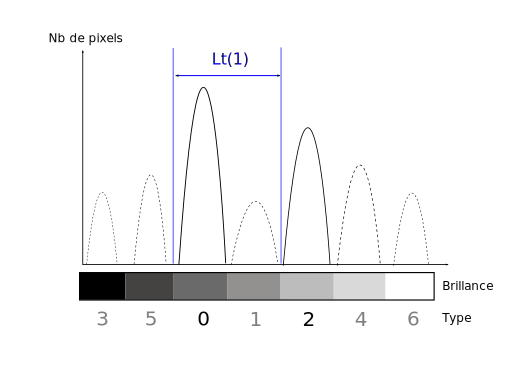
\includegraphics[trim= 0mm 5mm 0mm 5mm, clip, scale=0.3]{Formulation/figure/cas_1_histo.pdf}}	%trim=l b r t  width=0.5\textwidth, 
% 	      }\caption{Sous-ensemble non segmenté.}
%          \label{fig:contextual_info_rappel_ex}
% 	\end{figure}
% 	%%%%%%%%%%%%%%%%%%%%%%%%%%%%%%%%%%%%%%%%%%%%%%%%%%%

\begin{itemize}
\item Cas 4 : recherche du type $5$ sachant que les types 0, 2 et 4 ont été segmentés
\end{itemize}

	%%%%%%%%%%%%%%%%%%%%%%%%%%%%%%%%%%%%%%%%%%%%%%%%%%%
	\begin{figure}[!ht]	%trim=l b r t  width=0.5\textwidth,
	  \centering
	      \fbox{
		  \subfloat[Graphe $G_{T,t}$]{\label{fig:cas_4_graph_topo}\includegraphics[trim= 20mm 5mm 0mm 5mm, clip, scale=0.4]{Formulation/figure/cas_4_graph_topo.pdf}}
		  %\subfloat[Image masquée]{\label{fig:cas_2_img}\includegraphics[trim= 8mm 20mm 10mm 5mm, clip, scale=0.5]{Formulation/figure/cas_2_img.pdf}}
		  \subfloat[Histogramme]{\label{fig:cas_4_histo}\includegraphics[trim= 0mm 10mm 0mm 5mm, clip, scale=0.4]{Formulation/figure/cas_4_histo.pdf}}
		  \subfloat[Graphe $G_{P,t}$]{\label{fig:cas_4_graph_photo}\includegraphics[trim= -10mm 0mm -10mm 0mm, clip, scale=0.4]{Formulation/figure/cas_4_graph_photo.pdf}}
	      }\caption{Sous-ensemble $L_t(5)$.}
         \label{fig:cas_4}
	\end{figure}
	%%%%%%%%%%%%%%%%%%%%%%%%%%%%%%%%%%%%%%%%%%%%%%%%%%%

	%%%%%%%%%%%%%%%%%%%%%%%%%%%%%%%%%%%%%%%%%%%%%%%%%%%
% 	\begin{equation}
% 	\begin{split}
% 	  L_t(5) = & \left( ( S \setminus S_t ) \cap G_{T}^\infty \left( G_{T,t}^{-1} \left( 5 \right) \right) \right) \cup G_{T,t}^{-1}(5) \\
% 		= & \left( \{1,3,5,6\} \cap G_T^{\infty}(\{ 2,4 \}) \right) \cup \{ 2,4 \} \\
% 		= & \left( \{1,3,5,6\} \cap \{ 3,4,5,6\}\right) \cup \{ 2,4 \} \\
% 		= & \left\{ 3,5,6 \right\} \cup \{ 2,4 \} \\
% 		= & \left\{ 3,5,6,2,4 \right\}
% 	\end{split}
% 	\end{equation}
	%%%%%%%%%%%%%%%%%%%%%%%%%%%%%%%%%%%%%%%%%%%%%%%%%%%

% 	%%%%%%%%%%%%%%%%%%%%%%%%%%%%%%%%%%%%%%%%%%%%%%%%%%%
% 	\begin{equation}
% 	\begin{split}
% 	  %L_t(5) = & \left( ( S \setminus S_t ) \cap G_{T}^\infty \left( G_T^{-1}(5) \setminus G_{T,t}^{-1} \left( 5 \right) \right) \right) \cup G_{T,t}^{-1}(5) \\
% 	 L_t(5) = & \left( \left( G_T(i) \ni G_{T,t}(u)  \right) \;|\; i \in G_{T,t}^{-1}(u) \right) \cup G_{T,t}^{-1}(5) \\
% 		= & \left( \left( G_T(i) \ni G_{T,t}(5)  \right) \;|\; i \in G_{T,t}^{-1}(\{ 2,4 \}) \right) \cup G_{T,t}^{-1}(5) \\
% 		= & \left( \left( G_T(i) \ni \{0,2,4\}  \right) \;|\; i \in G_{T,t}^{-1}(\{ 2,4 \}) \right) \cup G_{T,t}^{-1}(5) \\
% 		= & \left( \{1,3,5,6\} \cap G_T^{\infty}(\{ 2,4 \}) \right) \cup \{ 2,4 \} \\
% 		= & \left( \{1,3,5,6\} \cap \{ 3,4,5,6\}\right) \cup \{ 2,4 \} \\
% 		= & \left\{ 3,5,6 \right\} \cup \{ 2,4 \} \\
% 		= & \left\{ 3,5,6,2,4 \right\}
% 	\end{split}
% 	\end{equation}
% 	%%%%%%%%%%%%%%%%%%%%%%%%%%%%%%%%%%%%%%%%%%%%%%%%%%%

	%%%%%%%%%%%%%%%%%%%%%%%%%%%%%%%%%%%%%%%%%%%%%%%%%%%
	\begin{equation}
	\begin{split}
	  %L_t(5) = & \left( ( S \setminus S_t ) \cap G_{T}^\infty \left( G_T^{-1}(5) \setminus G_{T,t}^{-1} \left( 5 \right) \right) \right) \cup G_{T,t}^{-1}(5) \\
	 L_t(5) = & \left\{ i \in \left( G_T^{\infty}(G_{T,t}^{-1}(5)) \cap ( S \setminus S_t ) \right)\;|\; \left( G_{T,t}^{-1} (i) \cap G_{T,t}^{-1} (5) \neq \emptyset \right) \right\} \cup  G_{T,t}^{-1}(5)\\
		= & \left\{ i \in \left( \{3,6,5\} \cap \{1,3,5,6\} \right)\;|\; \left( G_{T,t}^{-1} (i) \cap \{2,4\} \neq \emptyset \right) \right\} \cup  \{2,4\} \\
		= & \left\{3,6,5\} \cup \{ 2,4 \right\} \\
	\end{split}
	\end{equation}
	%%%%%%%%%%%%%%%%%%%%%%%%%%%%%%%%%%%%%%%%%%%%%%%%%%%

	Parmi les types non segmentés, le type 1 n'a pas de prédécesseur commun avec ceux de $u$, il est donc exclu (fig.~\ref{fig:cas_4_graph_topo}). Il reste donc 3, 6 et 5 ainsi que les prédécesseurs de $u$ : 2 et 4 (second membre). L'ensemble trouvé $L_t(5) = \{3,6,5,2,4\}$ (fig.~\ref{fig:cas_4_histo}). Sa cardinalité $N_t(4) = \left|{L_t(5)}\right| = 5$.\vspace{1em}

	%%%%%%%%%%%%%%%%%%%%%%%%%%%%%%%%%%%%%%%%%%%%%%%%%%%
%	\begin{equation}
% 	\begin{split}
% 	 L_t(5) = & \left\{ ( S \setminus S_t ) \cap ( G_T^{\infty}(U) \setminus G_T^{\infty} (G_{T,t}^{+1}(U) ) ) \right\} \cup U \\
% 	  %L_t(5) = & \left( ( S \setminus S_t ) \cap G_{T}^\infty \left( G_{T,t}^{-1} \left( 5 \right) \right) \right) \cup G_{T,t}^{-1}(5) \\
% 		= & \left( \{1,3,5,6\} \cap \left( G_T^{\infty}(\{ 2,4 \}) \setminus G_T^{\infty} ( G_{T,t}^{+1}(\{ 2,4 \}) )  				\right) \right) \cup \{ 2,4 \} \\
% 		= & \left( \{1,3,5,6\} \cap \left( G_T^{\infty}(\{ 2,4 \}) \setminus G_T^{\infty} ( G_{T,t}^{+1}(\{2\}) \cup G_{T,t}^{+1}(\{4\}) )  	\right) \right) \cup \{ 2,4 \} \\
% 		= & \left( \{1,3,5,6\} \cap \left( G_T^{\infty}(\{ 2,4 \}) \setminus G_T^{\infty} ( \{4\} 		\cup \emptyset )  		\right) \right) \cup \{ 2,4 \} \\
% 		= & \left( \{1,3,5,6\} \cap \left( G_T^{\infty}(\{ 2,4 \}) \setminus \{6,5\} )  							\right) \right) \cup \{ 2,4 \} \\
% 	        = & \left( \{1,3,5,6\} \cap \left( \{ 3,4,5,6\}\setminus \{6,5\}									\right) \right) \cup \{ 2,4 \} \\
% 	        = & \left( \{1,3,5,6\} \cap \left( \{ 3,4\}												\right) \right) \cup \{ 2,4 \} \\
% 		= & \left\{ 3,2,4 \right\} (ERROR!!!)
% 	\end{split}
% 	\end{equation}
	%%%%%%%%%%%%%%%%%%%%%%%%%%%%%%%%%%%%%%%%%%%%%%%%%%%


	%%%%%%%%%%%%%%%%%%%%%%%%%%%%%%%%%%%%%%%%%%%%%%%%%%%
% 	\begin{equation}
% 		%N_t(u) = \operatorname{Card}\{X_t(i) \in R_t(u) \; \forall \;i\}
% 		%L_t(4) = \{i \in S \setminus S_t \;|\; X(i) \in R_t(4) \; AND \; G_{P,t}^{[4,2]} \}
% 		L_t(5) = \{i \in S \setminus S_t \;|\; X(i) \in R_t(5)\} \cup \{ G_{T,t}^{-1}(5) \}
% 		%nbClMax = \operatorname{Card}\{R_t(u)\}
% 		\label{eq:lobes_cas_4}
% 	\end{equation}
	%%%%%%%%%%%%%%%%%%%%%%%%%%%%%%%%%%%%%%%%%%%%%%%%%%%

	%L'ensemble des types non segmentés $S \setminus S_t = \{1,3,5,6\}$, restreint à $R_t(5)$, 1 est éliminé (fig.~\ref{fig:cas_4_graph_topo}). Le deuxième membre $G_{T,t}^{-1}(5) = \{2,4\}$, 4 étant déjà considéré par le premier membre, $L_t(5) = \{3,5,6,2,4\}$. Cet ensemble est représenté sur l'histogramme~\ref{fig:cas_4_histo}. Sa cardinalité $N_t(5) = \left|{L_t(5)}\right| = 5$.

	%(Réponse à une ancienne note\footnote{Ancienne formule: à quoi correspond $S(i)$ dans ($S(i) \in G_{T}^\infty( j \in G_{T,t}^{-1}(u) )$) ? C'est une erreur, $S(i)=>i$ et $j$ est un type appartenant à l'ensemble des prédécesseurs de $u$. Par contre, ta formulation semble plutôt correcte. Je précise tout du moins quelques petites choses: à discuter ensemble})
%\newpage
\begin{itemize}
\item Cas 5 : recherche du type $1$ sachant que les types 0 et 4 ont été segmentés
\end{itemize}

	%%%%%%%%%%%%%%%%%%%%%%%%%%%%%%%%%%%%%%%%%%%%%%%%%%%
	\begin{figure}[!ht]	%trim=l b r t  width=0.5\textwidth,
	  \centering
	      \fbox{
		  \subfloat[Graphe $G_{T,t}$]{\label{fig:cas_5_graph_topo}\includegraphics[trim= 20mm 5mm 0mm 5mm, clip, scale=0.4]{Formulation/figure/cas_5_graph_topo.pdf}}
		  %\subfloat[Image masquée]{\label{fig:cas_2_img}\includegraphics[trim= 8mm 20mm 10mm 5mm, clip, scale=0.5]{Formulation/figure/cas_2_img.pdf}}
		  \subfloat[Histogramme]{\label{fig:cas_5_histo}\includegraphics[trim= 0mm 10mm 0mm 5mm, clip, scale=0.4]{Formulation/figure/cas_5_histo.pdf}}
		  \subfloat[Graphe $G_{P,t}$]{\label{fig:cas_5_graph_photo}\includegraphics[trim= -10mm 0mm -10mm 0mm, clip, scale=0.4]{Formulation/figure/cas_5_graph_photo.pdf}}
	      }\caption{Sous-ensemble $L_t(5)$.}
         \label{fig:cas_5}
	\end{figure}
	%%%%%%%%%%%%%%%%%%%%%%%%%%%%%%%%%%%%%%%%%%%%%%%%%%%


	%%%%%%%%%%%%%%%%%%%%%%%%%%%%%%%%%%%%%%%%%%%%%%%%%%%
	\begin{equation}
	\begin{split}
	 L_t(1) = & \left\{ i \in \left( G_T^{\infty}(G_{T,t}^{-1}(1))  \cap ( S \setminus S_t ) \right) \;|\; \left( G_{T,t}^{-1} (i) \cap G_{T,t}^{-1} (1) 	\neq \emptyset \right) \right\} \cup  G_{T,t}^{-1}(1)	\\
		= & \left\{ i \in \left( 	\{1,2,3,4,5,6\} 	\cap 	\{1,2,3,6,5\}	 \right) \;|\; \left( G_{T,t}^{-1} (i) \cap 	\{0\} 		\neq \emptyset \right) \right\} \cup  	\{0\}		\\
		= & \left\{ 1,2,3,5 \right\}																			\cup  	\{0\}
	\end{split}
	\end{equation}
	%%%%%%%%%%%%%%%%%%%%%%%%%%%%%%%%%%%%%%%%%%%%%%%%%%%

	Ici on teste le cas où les types n'ont pas été segmentés suivant l'ordre topologique. La formule reste robuste car on obtient bien l'ensemble des prédécesseurs de 1 avec leurs successeurs non segmentés à l'exception de 6 puisque il a pour prédécesseur $\{4\} \neq \{0\} = G_{T,t}^{-1}(1)$.

\begin{comment}

	%Une amélioration pourrait être que $L_t(u)$ soit l'union de l'ensemble des successeurs $i$, non actifs ($i \in S \setminus S_t$), de chacun des prédécesseurs directs "actifs" (\in $S_t$) de $u$ et des prédécesseurs de $u$ eux-mêmes.%l'ensemble des types $i$ non actifs ($i \in S \setminus S_t$) qui sont inclus dans
 	
% 	Une amélioration de $L_t(u)$ pourrait être, pour un élément $i$ issu des prédécesseurs de $u$ ($i\in G_{T,t}^{-1}(u)$), l'union de l'ensemble des successeurs non segmentés ($G_T^{\infty}(i) \cap \{S \setminus S_t\}$) et des prédécesseurs de $u$ eux-mêmes ($G_{T,t}^{-1}(u)$).%.    (i.e. éléments de $S \setminus S_t$) et des prédécesseurs de $u$ (i.e. $G_{T,t}^{-1}(u)$).   soit l'union de l'ensemble des successeurs $i$, non actifs ($i \in S \setminus S_t$), de chacun des prédécesseurs directs "actifs" de $u$ ($G_{T,t}^{-1}(u)$) et des prédécesseurs de $u$ eux-mêmes ($G_{T,t}^{-1}(u)$). %l'ensemble des types $i$ non actifs ($i \in S \setminus S_t$) qui sont inclus dans
% 
% 	%{\bf L'ensemble des prédécesseurs directs "actifs" de $u$ est: $G_{T,t}^{-1}(u)$}
% 
% 	L'union de l'ensemble de ses successeurs non segmentés d'un type $k$ ($G_T^{\infty}(k) \cap \{S \setminus S_t\}$) peut être également noté $\{ k\in S \setminus S_t|\; k \in G_T^{\infty}(i)\}$.
% 
% 	%{\bf Pour un élément $i$ donné de ces prédécesseurs (i.e. $i\in G_{T,t}^{-1}(u)$), l'ensemble des successeurs non valides (i.e. éléments de $S \setminus S_t$) peut être noté: $G_T^{\infty}(i) \cap \{S \setminus S_t\}$ ou $\{ k\in S \setminus S_t|\; k \in G_T^{\infty}(i)\}$.}
% 
% 	On peut en déduire la formule suivante pour $L_t(u)$, sans explicitement utilisé la ROI:
% 
% \begin{equation}
% L_t(u) =  \left(\bigcup_{i\in G_{T,t}^{-1}(u)} \{ k\in S \setminus S_t|\; k \in G_T^{\infty}(i)\} \right) \cup \left\{ G_{T,t}^{-1}(u) \right\}
% \end{equation}
% 
% %{\bf On peut introduire la notion de prédécesseurs-successeurs d'un ensemble de noeuds, e.g. $G_{T}^\infty(G_{T,t}^{-1}(u) )$ (à introduire dans le glossaire des notations comme étant l'union des prédécesseurs-successeurs de chacun des éléments de l'ensemble).}
% La formule précédente se simplifie :
% \begin{equation}
% L_t(u) =  \{ i\in S \setminus S_t|\; i \in G_T^{\infty}(G_{T,t}^{-1}(u))\} \cup G_{T,t}^{-1}(u)
% \end{equation}
% 
% C'est à dire :
% 
% \begin{equation}
% L_t(u) = \left\{ ( S \setminus S_t ) \cap  G_T^{\infty}(G_{T,t}^{-1}(u)) \right\} \cup G_{T,t}^{-1}(u)
% \end{equation}
% 

%{\bf L'ensemble de recherché est $\{i \in S \setminus S_t |\; dsqf\}$ prédécesseurs directs "actifs" de $u$ est: $G_{T,t}^{-1}(u)$}

% \begin{itemize}
% \item Application au cas 3:
% \end{itemize}
% \begin{equation}
% L_t(4) = \left( ( S \setminus S_t ) \cap  G_T^{\infty}(G_{T,t}^{-1}(4)) \right) \cup G_{T,t}^{-1}(4)
% \end{equation}
% \begin{equation}
% L_t(4) = \left(\{1,4\} \cap G_T^{\infty}(\{2\})\right) \cup \{ 2 \}
% \end{equation}
% \begin{equation}
% L_t(4) =   \left(\{1,4\} \cap \{ 3,4,5,6\}\right) \cup \{ 2 \}
% \end{equation}
% \begin{equation}
% L_t(4) =   \{ 4\} \cup \{ 2 \} =   \{ 4,2 \}
% \end{equation}


% \begin{equation}
% L_t(5) = \left( ( S \setminus S_t ) \cap  G_T^{\infty}(G_{T,t}^{-1}(5)) \right) \cup G_{T,t}^{-1}(5)
% \end{equation}
% \begin{equation}
% L_t(5) = \left( \{1,3,5,6\}  \cap G_T^{\infty}(\{2,4\}) \right) \cup \{2,4\}
% \end{equation}
% \begin{equation}
% L_t(5) =  \left( \{1,3,5,6\} \cap \{3,4,5,6\} \right) \cup \{2,4\}
% \end{equation}
% \begin{equation}
% L_t(5) =  \{3,5,6\} \cup \{2,4\} = \{3,5,6,2,4\}
% \end{equation}





%($S(i) \in G_{T}^\infty( j \in G_{T,t}^{-1}(u) )$). Ainsi que le prédécesseur lui même ($G_{T,t}^{-1}(u)$). %Pour que cette amélioration s'applique dans le cas où $u$ a plusieurs prédécesseurs direct actifs on considérera l'union de ces prédécesseurs ($\bigcup{ G_{T,t}^{-1}(u)}$).

% potientielle à fournir sur $L_t$ serait de plus dépendre des régions de l'image dans la formulation, mais seulement des noeuds du graphe (facilitera également l'implémentation). La formule actuelle devra être conservée comme formule intermédiaire permettant de mieux comprendre la démarche par rapport à la ROI.}
% {\bf Ci-après: ta version : je l'ai laissé temporairement: peut-être à enlever si pertinent après validation ensemble.}
% \begin{itemize}
% \item Application au cas 3:
% \end{itemize}
% 	%%%%%%%%%%%%%%%%%%%%%%%%%%%%%%%%%%%%%%%%%%%%%%%%%%%
% 	\begin{equation}
% 		L_t(u) = \left\{i \in S \setminus S_t \;|\; i \in G_{T}^\infty \left( j \in G_{T,t}^{-1}\left( u \right) \right) \right\} \cup \left\{ G_{T,t}^{-1}(u) \right\}
% 		\label{eq:new}
% 	\end{equation}
% 	%%%%%%%%%%%%%%%%%%%%%%%%%%%%%%%%%%%%%%%%%%%%%%%%%%%
% 	
% 	Avec :
% 
% 	\begin{itemize}
% 	  \item $S \setminus S_t = \{1,4\}$
% 	  \item $G_{T,t}^{-1}\left( 4 \right) = \{2\}$
% 	  \item $G_{T}^\infty \left( 2 \right)=\{3,4,6,5\}$
% 	\end{itemize}
% 
% 	%%%%%%%%%%%%%%%%%%%%%%%%%%%%%%%%%%%%%%%%%%%%%%%%%%%
% 	\begin{equation}
% 	\begin{split}
% 	  L_t(4) = & \left\{ i \in S \setminus S_t \;|\; i \in G_{T}^\infty \left( j \in G_{T,t}^{-1}\left( 4 \right) \right) \} \cup \{ G_{T,t}^{-1}(4) \} \right. \\
% 		= & \left\{ i \in \{1,4\} \;|\; i \in \{3,4,6,5\} \cup \{ 2 \} \right. \\
% 		= & \left.\{ 4, 2 \right\}
% 	\end{split}
% 	\end{equation}
% 	%%%%%%%%%%%%%%%%%%%%%%%%%%%%%%%%%%%%%%%%%%%%%%%%%%%
% 
% \begin{itemize}
% \item Application au cas 4:
% \end{itemize}
% 	Application de la formule améliorée :
% 	%%%%%%%%%%%%%%%%%%%%%%%%%%%%%%%%%%%%%%%%%%%%%%%%%%%
% 	\begin{equation}
% 	\begin{split}
% 	  L_t(5) = &\left. \{ i \in S \setminus S_t \;|\; i \in G_{T}^\infty \left( j \in G_{T,t}^{-1}\left( 5 \right) \right) \} \cup \{ G_{T,t}^{-1}(5) \} \right. \\
% 		= & \left. \{ i \in \{1,3,6,5\} \;|\; i \in \{3,4,6,5\} \cup \{ 4,2 \} \right. \\
% 		= & \left. \{ 3,6,5,4,2\} \right. \\
% 		  & \left. \right. \\
% 	  N_t(5)= & \left. \operatorname{card}\{L_t(5)\} \right. \\
% 		= & \left. \operatorname{card}\{3,6,5,4,2\} \right. \\
% 		= & \left. 5 \right.
% 	\end{split}
% 	\end{equation}
% 	%%%%%%%%%%%%%%%%%%%%%%%%%%%%%%%%%%%%%%%%%%%%%%%%%%%
% 
% 	Avec :
% 
% 	\begin{itemize}
% 	  \item $S \setminus S_t = \{1,3,6,5\}$
% 	  \item $G_{T,t}^{-1}\left( 5 \right) = \{4,2\}$
% 	  \item $G_{T}^\infty \left( 4 \right)=\{6,5\}$
% 	  \item $G_{T}^\infty \left( 2 \right)=\{3,4,6,5\}$
% 	\end{itemize}
\end{comment}

%\newpage

% \newpage
% \begin{itemize}
% \item Cas 7 : recherche du type $6$ sachant que les types 0, 2, 4 et 6 ont été segmentés et que tous les types 6 sont segmentés : 
% \end{itemize}

	%A venir...\hspace{1em}
	%\textit{Dans le cas de la multiplicité, cela se transformera peut-être en un intervalle, i.e. un nombre min et max de lobe, permettant tout de même d'apporter des informations sur le nombre de classes min et max à utiliser pour la recherche de lobe avec gaussian mixture... le travail deviendra intéressant: il y aura une recherche d'un nombre classe optimal entre un min et un max (fonction de l'erreur d'estimation)... On verra plus tard comment ajuster la formule 1.3 pour qu'elle reste valable dans les deux cas.}


%     \subsubsection*{Caractère optionnel des types (0 ou 1)}

%	L'aspect optionnel des types dans l'image est dû aux type de structures (e.g.pathologiques). Si des types sont considérés comme optionnels, l'ensemble $L_t(u)$ deviendra de taille variable et influencera directement $N_t(u)$. On pourra dire que $N_t(u) \in \left[a, b\right]$ avec $a$ et $b$ les valeurs minimale et maximale de $N_t(u)$.
	%Appliqué à notre cas : $N_t(6) = \left[ \min{ \operatorname{card}\{L_t(6)\}}, \max{\operatorname{card}\{L_t(6)\}} \right] = \left[1, 3 \right]$.

\newpage
      \subsection{Identification des lobes}
	Nous identifions les lobes (correspondant aux classes de l'image) présentes dans l'image pour pouvoir optimiser le fenêtrage de la structure recherchée. L'identification consiste en l'ordonnancement des lobes de l'ensemble $L_t$ en fonction de leur intensité lumineuse. Dans cette étude, et sous l'hypothèse d'une distribution des intensités selon un loi normale, ``plus sombre'', se traduira par la moyenne (de la gaussienne) des intensités de $i$ est inférieure à la moyenne des intensités de $j$. On s'appuie sur les relations photométriques inter-types que l'on représente par un graphe (voir fig.~\ref{fig:info_photo_graph}) dont des arcs orientés signifient ``plus sombre que''. On utilise ensuite l'opérateur \texttt{ord} qui comparera les relations photométriques inter-type jusqu'à l'obtention d'une suite de types ordonnés par intensité moyenne croissante. On exprime cette opération par :


	%%%%%%%%%%%%%%%%%%%%%%%%%%%%%%%%%%%%%%%%%%%%%%%%
% 	\begin{equation}
% 		%N_t(u) = \operatorname{Card}\{X_t(i) \in R_t(u) \; \forall \;i\}
% 		L_{t,i}(u) = \operatorname{ord} \{ L_t(u) \} \; \forall \; i,j \in L_t(u)
% 		%nbClMax = \operatorname{Card}\{R_t(u)\}
% 		\label{eq:lobes}
% 	\end{equation}

	\begin{equation}
		O_t(u) = \operatorname{ord} \{ L_t(u) \} = \{ L_{t,i}(u) \; |\; i \in \{0,...,N_t-1\} \}
		\label{eq:8}
	\end{equation}
	%%%%%%%%%%%%%%%%%%%%%%%%%%%%%%%%%%%%%%%%%%%%%%%%

	Cet ensemble est ordonné, ce qui signifie que, $\forall (i,j) \in \{0,...,N_t-1\}^2\; |\; \left( L_{t,i}\left(u\right),L_{t,j}\left(u\right)\right) \in \left( O_t\left(u\right), L_{t,i}\left(u\right) < L_{t,j}\left(u\right)\right)$ \footnote{La relation $\in O, L < L$ ne me semble pas claire, est-ce vraiment la représentation standard pour un ensemble ordonné et sont opérateur? Ne doit-on pas plutôt utiliser des accolades quand on parle d'ensemble?} :
	%({\bf finalement, il est peut-être préférable de retirer la notion de comparaison entre région (i.e. la formule $X(i)< X(j)$ présente dans la précédente version), car il peut y avoir ambiguïté avec une relation de taille entre les régions. Bilan: ce qui suit me paraît suffisant})
	\begin{itemize}
		\item
		En terme d'image: la région $X(i)$ est plus sombre que la région $X(j)$
		\item
		En terme de graphe: le noeud $i$ est prédécesseur de $j$ dans le graphe $G_{P} \Rightarrow i \in G_{P,t}^{-\infty}(j)$
	\end{itemize}

	%Remarque à placer quelque part: la notion "$i$ est plus sombre que la région $j$" signifie que, globalement, la région $i$ est plus sombre que la région $j$. "Globalement" car certains point de la région $i$ peuvent être plus clairs que certains autres points de la région $j$ (e.g. récouvrement des lobes). Dans cette étude, et sous l'hypothèse d'une distribution des intensités selon un loi normale, "plus sombre" se traduira par la moyenne (de la gaussienne) des intensités de $i$ est inférieure à la moyenne des intensités de $j$.

	%%%%%%%%%%%%%%%%%%%%%%%%%%%%%%%%%%%%%%%%%%%%%%%%%%%
	\begin{figure}[!ht]
	  \centering
	      \fbox{
		  \subfloat[Graphe $G_{P_t}$]
		  {\label{fig:info_photo_graph}
\includegraphics[trim= 0mm 0mm 0mm 5mm, clip, scale=0.3]{Formulation/figure/info_photo_a_priori.pdf}}
		  \subfloat[Lobes identifiés]
		  {\label{fig:ident_histo}\includegraphics[trim= 0mm 5mm 0mm 5mm, clip, scale=0.3]{Formulation/figure/ident_histo.pdf}}	%trim=l b r t
	      }\caption{Exemple de représentation des informations photométriques ($G_{P,t}$) correspondant au cas n$^{\circ}$2 énoncé plus haut.}
         \label{fig:info_photo_a_priori}
	\end{figure}
	%%%%%%%%%%%%%%%%%%%%%%%%%%%%%%%%%%%%%%%%%%%%%%%%%%%

	Appliqué au cas n$^{\circ}$2, $O_t(3)$ compare la relation photométrique entre les types de l'ensemble $L_t(3) = \{2,3,4,5,6\}$ deux à deux, c.a.d. chaque type {\bf $i\in L_t(3)$} va être comparé à un autre type $j\in L_t(3)$ itérativement. 
	
	Selon~\ref{fig:info_photo_graph}, 2 est plus clair que 3 qui est plus sombre que 5 et ainsi de suite $\Rightarrow O_t(3) = \{3,5,2,4,6\}$. Le premier lobe de l'histogramme ~\ref{fig:ident_histo} est donc identifié comme étant de type 3, le second de type 5 et ainsi de suite sachant que 0 et 1 sont exclut de $L_t(3)$.

\newpage
	\section{Discussion: limites et perspectives}

	Dans la formulation dédiée à la photométrie (section~\ref{sec:inf_and_photo}), nous avons considéré des régions avec une multiplicité de 1. Cette hypothèse simplificatrice signifie que nous avons ignoré les situations suivantes:
\begin{itemize}
\item le caractère optionnel d'une région (e.g. une tumeur peut être absente bien que représentée dans le graphe) ;
\item le caractère multiple d'une région : ceci peut notamment concerner le cas de tumeurs multiples, chacune d'elles étant segmentée à une étape différente du processus d'analyse ;
\item le cas où une région $A$ contient des sous-régions dont l'union occupe toute la région $A$ : il n'y alors aucune classe (lobe de l'histogramme) qui correspond spécifquement à la région $A$.
\end{itemize}\vspace{1em}

	Contrairement au cas de la ROI \citep[Fasquel]{Fasquel2006}, cet aspect a un impact sur les déductions faites par le moteur d'inférence comme le nombre de classes. Ce choix est justifié par le fait que la formalisation proposée apparaît, comme constaté dans les sections précédentes, relativement complexe, malgré cette hypothèse simplificatrice. Ceci justifie donc de débuter l'étude dans un cas simple même si l'hypothèse simplificatrice peut s'avérer très limitante d'un point de vue applicatif (e.g. cas précédemment cité des tumeurs). 

	L'élimination de cette hypothèse nécessite de poursuivre l'étude, ce qui aurait probablement pour conséquence de modifier le formalisme présenté, notamment concernant la détermination du nombre de classe qui conduirait non plus à une valeur exacte mais probablement à un intervalle (e.g. selon qu'une tumeur est présente ou non, le nombre de classe peut varier entre un minimum et un maximum).
	
	Nous avons fait le choix d'évaluer cette première phase de l'étude en priorité afin d'en discuter des bénéfices, plutôt que d'étendre davantage le formalisme. Le bilan de cette partie est que la formalisation n'est pas triviale, contrairement à ce que l'on pourrait intuitivement penser en première approche, et qu'une étude des bénéfices semble pertinente avant de légitimer un effort de formalisation supplémentaire.

	Néanmoins, avant de détailler les études relatives à cette évaluation, nous présentons succinctement quelques pistes qui pourraient être envisagées dans le cas d'une multiplicité supérieure à 1. Le caractère optionnel (multiplicité 0) n'ayant pas été abordé.
	
%{\bf Ce travail a, pour le moment été limité où une région est supposée présente dans l'image, sans caractère optionnel. En effet, on peut considérer qu'un noeud du graphe peut être associé à une ou plusieurs régions (région "multiple"), segmentées à des étapes distinctes du processus d'analyse. Dans le cadre d'images médicales, ceci peut s'apparenter à la présence de plusieurs tumeurs, pouvant être segmentées à différentes étapes du processus d'analyse. Nous considérerons ci-après le cas d'une multiplicité égale à 1 et ensuite le cas d'une multiplicité supérieure à 1. Nous faisons l'hypothèse simplificatrice que les propriétés photométriques associées à une noeud sont constantes, même en cas de multiplicité supérieure à 1. D'un point de vue pratique, ceci signifie que différentes régions associées à un même noeud auront par exemple la même intensité moyenne et le même écart-type. 

%Le cas non traité ici concerne une multiplicité nulle, relatif à une région dont la présence n'est pas certaine (e.g. une tumeur). Cet aspect pourrait faire l'objet d'une étude complémentaire.}


%		Le moteur d'inférence agit comme une interface entre les informations à priori (à renseigner manuellement) et leur traitement selon le formalisme définis ci-dessus. Dans la suite du document, on l'utilisera comme un système d'information qui renvoi une réponse en fonction de ce qu'on lui infère. 

 
%      \subsection{A conserver ? Cas de multiplicité de 1 à N types similaires}	% de $\mathbb{N}$}
	Une piste envisageable repose sur l'ajout d'un attribut (nous le noterons $M$) à chaque noeud du graphe, spécifiant la multiplicité potentielle d'une région. Une limitation de cette approche concerne l'élément quantitatif introduit dans la représentation des connaissances, sachant que nous privilégions une représentation des connaissances non quantitative dans la méthode proposée. Dans ce contexte, nous ferons l'hypothèse que les différentes régions d'une même classe ($M$>1) présentent les mêmes propriétés photométriques.\\

%	Ici nous considérons que tous les types $\in S$ peuvent avoir un caractères multiples $M(i)$ (e.g. pathologie identique et multiple). La multiplicité, notée $M$ ici, fait partie des connaissances topologiques à priori. Une multiplicité de $N$, signifie que chaque type peut apparaître plusieurs fois dans l'image, il peut donc y avoir deux ou plusieurs tumeurs hépatiques par exemple. On pourra interpréter cette information comme la présence de deux types photométriquement identiques (sous l'hypothèse qu'ils ont la même distribution) et spatialement différents. 

%Nous rappelons que ce cas peut par exemple être rencontré lorsque, après la segmentation de la région d'intérêt d'un type $u$, un nouveau type identique à $u$ apparaîtra dans l'histogramme de l'image dans le même intervalle d'intensité que $u$. 

%%%%%%%%%%%%%%%%%%%%%%%%%%%%%%%%%%%%%%%%%%%%%%%%%%%%%%%%%%%%%%%%%%%%%%%%%%%%%%%%%%%%%%%%%%%%%%%%%%%%%%%%%%%%%%%%%%%%%%%%%%%%%
%														MULTIPLICITE														%
%%%%%%%%%%%%%%%%%%%%%%%%%%%%%%%%%%%%%%%%%%%%%%%%%%%%%%%%%%%%%%%%%%%%%%%%%%%%%%%%%%%%%%%%%%%%%%%%%%%%%%%%%%%%%%%%%%%%%%%%%%%%%

%{\bf CI-DESSOUS: NE PAS LE METTRE DANS LA PRESENTATION POUR LE MOMENT CAR IL N'EST PAS CERTAIN QUE CE SOIT CONSERVÉ.\\}

%Ceci signifie que nous devons donc inclure, au sous-ensemble $L_t(u)$ présenté précédemment, les types déjà segmentés $\in S_t$ qui ont une multiplicité $>$ 1 car ils seront présent dans l'image. Le niveau de multiplicité $M(i)$ devra être décrémenté à chaque segmentation du type $u$ pour converger vers la forme précédente de $L_t(u)$ lorsque il sera égal à 0 ou 1.\\
%	Complétons le sous-ensemble $L_t$ en ajoutant les types déjà segmentés ayant une multiplicité $>$ 1 pour considérer les lobes résiduelles après la segmentation :

%	%%%%%%%%%%%%%%%%%%%%%%%%%%%%%%%%%%%%%%%%%%%%%%%%
%	\begin{equation}
%	  \begin{split}
%	    Lm_t(u) = & L_t(u)  \cup  \left\lbrace i \in G_{T,t}^{\infty} \left(G_{T,t}^{-1} \left(u \right) \right) | M(i) > M_t(i) \right\rbrace
%	  \end{split}
%	  \label{eq:subset_multiple_2_n}
%	\end{equation}\vspace{1em}
%	%%%%%%%%%%%%%%%%%%%%%%%%%%%%%%%%%%%%%%%%%%%%%%%%

%\begin{itemize}
%\item Cas 1 : recherche du type $6$ sachant que les types 0, 2 et 4 ont été segmentés et qu'il y a au moins deux structures non segmenté de type 6 présentent dans l'image ($M(6) > 2$) :
%\end{itemize}

%	%%%%%%%%%%%%%%%%%%%%%%%%%%%%%%%%%%%%%%%%%%%%%%%%%%%
%	\begin{figure}[!ht]	%trim=l b r t  width=0.5\textwidth,
%	  \centering
%	      \fbox{
%		  \subfloat[Graphe $G_T,t$]{\label{fig:cas_1_n_graph_topo}\includegraphics[trim= 20mm 5mm 0mm 5mm, clip, scale=0.4]{Formulation/figure/cas_1_n_graph_topo.pdf}}
%		  \subfloat[Image synthétique]{\label{fig:cas_1_n_img}\includegraphics[trim= 5mm 20mm 5mm 5mm, clip, scale=0.5]{Formulation/figure/cas_1_n_img.pdf}}
%		  \subfloat[Histogramme]{\label{fig:cas_1_n_histo}\includegraphics[trim= 0mm 10mm 0mm 5mm, clip, scale=0.5]{Formulation/figure/cas_1_n_histo.pdf}}
%		  %\subfloat[Graphe $G_{P,t}$]{\label{fig:cas_4_graph_photo}\includegraphics[trim= -10mm 0mm -10mm 0mm, clip, scale=0.4]{Formulation/figure/cas_4_graph_photo.pdf}}
%	      }\caption{Sous-ensemble $L_t(6)$.}
%         \label{fig:cas_1_n}
%	\end{figure}
%	%%%%%%%%%%%%%%%%%%%%%%%%%%%%%%%%%%%%%%%%%%%%%%%%%%%

%	%%%%%%%%%%%%%%%%%%%%%%%%%%%%%%%%%%%%%%%%%%%%%%%%%%%
%	\begin{equation}
%	\begin{split}
%	  Lm_t(6) = & L_t(6)  \cup  \left\lbrace i \in G_{T,t}^{\infty} \left(G_{T,t}^{-1}(u) \right) | M(i) > M_t(i) \right\rbrace \\
%		= & \{5,4,6\}  \cup  \left\lbrace i \in \{\emptyset\} | 2 > 0 \right\rbrace \\
%		= & \{5,4,6\}  \cup  \{6\} \\
%	\end{split}
%	\end{equation}
%	%%%%%%%%%%%%%%%%%%%%%%%%%%%%%%%%%%%%%%%%%%%%%%%%%%%

%	Le nombre de lobes $N_t(6) = \left|{L_t(6)}\right| = \left|{5,6,4}\right| = 3$. Ici le type 6 peut être multiple sans changer le résultat car il n'est pas segmenté donc déjà inclus dans $L_t(6)$. Notons que dans l'histogramme~\ref{fig:cas_1_n_histo} tous les types 6 sont confondus sous un unique lobe à ce stade de la segmentation.\vspace{1em}

%\begin{itemize}
%\item Cas 2 : recherche du type $6$ sachant que les types 0, 2, 4 et 6 ont été segmentés une fois ($M_t(6)=1$) et que 6 a une multiplicité de 2 ($M(6)=2$) dans l'image : 
%\end{itemize}

%	%%%%%%%%%%%%%%%%%%%%%%%%%%%%%%%%%%%%%%%%%%%%%%%%%%%
%	\begin{figure}[!ht]	%trim=l b r t  width=0.5\textwidth,
%	  \centering
%	      \fbox{
%		  \subfloat[Graphe $G_T,t$]{\label{fig:cas_2_n_graph_topo}\includegraphics[trim= 20mm 5mm 0mm 5mm, clip, scale=0.4]{Formulation/figure/cas_2_n_graph_topo.pdf}}
%		  \subfloat[Image synthétique]{\label{fig:cas_2_n_img}\includegraphics[trim= 5mm 20mm 5mm 5mm, clip, scale=0.6]{Formulation/figure/cas_2_n_img.pdf}}
%		  \subfloat[Histogramme]{\label{fig:cas_2_n_histo}\includegraphics[trim= 0mm 10mm 0mm 15mm, clip, scale=0.5]{Formulation/figure/cas_2_n_histo.pdf}}
%	      }\caption{Sous-ensemble $L_t(6)$.}
%         \label{fig:cas_2_n}
%	\end{figure}
%	%%%%%%%%%%%%%%%%%%%%%%%%%%%%%%%%%%%%%%%%%%%%%%%%%%%

%	%%%%%%%%%%%%%%%%%%%%%%%%%%%%%%%%%%%%%%%%%%%%%%%%%%%
%	\begin{equation}
%	\begin{split}
%	  Lm_t(6) = & L_t(6) \cup \left\lbrace i \in G_{T,t}^{\infty} \left({ G_{T,t}^{-1} (6) }\right) | M(i) > M_t(i) \right\rbrace \\ 
%		= & \{5,4\} \cup \left\lbrace i \in \{6\} \;|\; 2 > 1 \right\rbrace \\ 
%		= & \{5,4,6\}
%	\end{split}
%	\end{equation}
%	%%%%%%%%%%%%%%%%%%%%%%%%%%%%%%%%%%%%%%%%%%%%%%%%%%%

%	Le nombre de lobes $N_t(6) = \left|{L_t(6)}\right| = \left|{\{5,4,6\}}\right| = 3$. Le type 6 a bien été ajouté par le nouveau membre de la formule ~\ref{eq:subset_multiple_2_n}. Il est toujours présent dans $Lm_t(6)$, malgré qu'il est déjà été segmenté une fois, puisque la condition $M(6) > M_t(6)$ est vérifiée. Cela signifie que toutes les structures de types 6 n'ont pas encore été segmentées et donc apparaîtront dans l'image~\ref{fig:cas_2_n_img} et l'histogramme~\ref{fig:cas_2_n_histo}. Si on segmentait de nouveau le type 6, la condition $M(6) > M_t(6)$ ne serait plus vérifiée puisque $M_t(6)=2$ et donc $L_t(6)=\{ 5,4 \}$. \vspace{1em}
%		
%		
%		
			

	%COMPILATION: 
%clear; bibtex main.aux;pdflatex main.tex ;evince main.pdf &


%%%%%%%%%%%%%%%%%%%%%%%%%%%%%%%%%%%%%%%%%%%%%%%%%%%%%%%%%%%%%%%%%%%%%%%%%%%%%%%%%%%%%%%%%%%%%%%%%%%%%%%%%%%%%%%%%%%%%
%													INTERET METHODE													%
%%%%%%%%%%%%%%%%%%%%%%%%%%%%%%%%%%%%%%%%%%%%%%%%%%%%%%%%%%%%%%%%%%%%%%%%%%%%%%%%%%%%%%%%%%%%%%%%%%%%%%%%%%%%%%%%%%%%%
	
\chapter{Évaluation}
\label{sec:eval}
	L'objectif de cette partie est d'évaluer les bénéfices des connaissances à priori présentées dans le chapitre~\ref{chap:info_concept} (la région d'intérêt, le nombre de classes et les relations d'ordre). Elles sont déduites des représentations conceptuelles des connaissances topologiques et photométriques, dans le cas d'une analyse séquentielle.\\

Intuitivement, l'information topologique permet :

%	Dans le chapitre précédent (chap.~\ref{chap:info_concept}), nous avons mis en place les mécanismes du moteur d'inférence via le formalisme. Nous allons maintenant le mettre en application pour analyser des images numériques synthétiques puis médicales. Notre méthode illustrée figure~\ref{fig:method_schema}, repose sur plusieurs éléments, tout d'abord, de part les informations à priori topologiques ($G_T$), nous allons pouvoir appliquer des masques successifs à l'image (définis par le moteur d'inférence) pour :

\begin{itemize}
	\item[a)] d'éliminer les données polluantes : amélioration du pourcentage de données utiles ;
	\item[b)] réduire le volume des données à traiter : complexité et temps de calcul réduits.
\end{itemize}

%Ensuite, nous travaillerons sur l'histogramme de l'image restreint à la \gls{ROI} pour segmenter et identifier chaque classe puis ajuster le fenêtrage pour une classe particulière (la cible). Nous nous appuierons cette fois ci sur les informations photométriques à priori ($G_P$), toujours issues du moteur d'inférence. Ces informations nous permettent de :
L'information photométrique permet de :

\begin{itemize}
	\item[c)] connaître le nombre et l'ordre des classes à priori : paramétrage des algorithmes de segmentation ;
	\item[d)] initialiser les algorithmes de segmentation au plus proche des paramètres des classes attendues (moyenne, intervalle) : moins d'itérations lors de la segmentation.
\end{itemize}\vspace{1em}

	A partir de ces considérations intuitives, nous proposons d'effectuer un certain nombre de tests permettant d'illustrer quantitativement les bénéfices. Il s'agit d'un exercice délicat, comparativement aux procédures classiques d'évaluation de la performance de classification d'un algorithme de segmentation (e.g. mesure objective du taux de pixel correctement classés). En effet, dans notre contexte, cette évaluation ne dépend pas seulement de la nature des données, mais également de l'algorithme et de la procédure itérative d'analyse (la région d'intérêt varie à chaque itération). Par conséquent, ces mesures quantitatives reflètent probablement moins objectivement les bénéfices de notre approche que dans le cas d'un algorithme particulier. 

	Notre objectif prioritaire est de montrer des cas dans lesquels notre approche facilite le traitement, afin d'alimenter notre argumentaire, et ainsi, de discuter des affirmations précédentes, dans des cas concrets. Cette démarche sera poursuivie dans un cadre plus applicatif dans le chapitre suivant dédié à une application médicale.

	Après une courte présentation de l'algorithme utilisé pour réaliser cette évaluation, nous allons traiter chacun des points cités précédemment (a, b, c, d).
%Nous allons illustrer chacun de ces points par un exemple simple, même si certain paraissent logiques, afin de quantifier le bénéfice attendu pour notre application.

	%%%%%%%%%%%%%%%%%%%%%%%%%%%%%%%%%%%%%%%%%%%%%%%%%%%%%%%%%%%%%%%%%%%%%%%%%%%%%%%%%%%%%%%%%%%%%%%%%%%%%%%%%%%%%%%%%%%%%
	%													CHOIX OUTILS													%
	%%%%%%%%%%%%%%%%%%%%%%%%%%%%%%%%%%%%%%%%%%%%%%%%%%%%%%%%%%%%%%%%%%%%%%%%%%%%%%%%%%%%%%%%%%%%%%%%%%%%%%%%%%%%%%%%%%%%%
	\section{Algorithme considéré}
		%Suite à l'état de l'art sur les techniques de seuillage d'images (section~\ref{sec:state_of_the_art}), 
Nous avons choisi d'utiliser l'algorithme des \emph{K-Means} car il est largement répandu pour les raisons évoquées dans \citep[Ranjan]{Ranjan2010} ``\textit{the simplicity and computational speed of the K-means algorithm ... has made it a popular choice.}''. Cet algorithme nécessite néanmoins des paramètres d'initialisations pour calculer une segmentation pertinente \citep[Ranjan]{Ranjan2010} ``\textit{the algorithm needs initializing values which greatly influence its terminating optimal solution ... good initialization is crucial for finding globally optimal partitionings}''. 
		
		L'algorithme \emph{K-Means} est une méthode dont le but est de diviser $n$ observations $X$ en $k$ partitions (clusters) $V=\{V_1, V_2, …, V_k\}$ afin de minimiser la somme des carrés à la moyenne à l'intérieur de chaque partition (eq.~\ref{eq:kmean}).
		
		
		%vise à partitionner un nuage de données en plusieurs ensembles de points (clusters) en minimisant la somme des carrés à la moyenne à l'intérieur de chaque partition.


 \begin{equation}
 	\mathrm{arg\;min} \sum_{j=1}^k \sum_{n \in V_j} \left| X_n - \mu_j \right|^2
 	\label{eq:kmean}
 \end{equation}
  
% et d'autre part, parce qu'il détermine les bornes minimum et maximum d'un groupe de points : ce qui est précisément ce dont nous avons besoin pour fenêtrage.

	Les paramètres sont : le nombre de partitions $k$ et leurs moyennes respectives. Nous déterminerons $k$ par les connaissances contextuelles à priori. Pour l'initialisation des moyennes, on peut utiliser des moyens automatiques comme le tirage aléatoire de valeurs, l'algorithme \emph{K-Means++}\citep[Arthur2007]{Arthur2007} ou bien manuellement. %Nous préférerons, dans la mesure du possible, une initialisation manuelle à partir des connaissances à priori pour s'assurer d'un résultat optimal (et invariable).

	Le contexte d'utilisation de cet algorithme s'apparente à de la segmentation d'images par analyse d'histogramme (analyse de la distribution des intensités). Il s'agit d'une approche couramment considérée en traitement d'images, l'enjeu étant la détermination robuste des seuils discriminant les différentes régions d'une image (\citep[Coudray]{Coudray2010}, \citep[Bhattacharyya]{Bhattacharyya2011}, \citep[Cheng]{Cheng1998}, \citep[Cuevas]{Cuevas2010}). Le lecteur pourra également se référer à l'état de l'art de \citep[Zhang]{Zhang2008} sur ces méthodes.

	\vspace{1em}
		
		%{\bf Figure de la méthode supprimée : à voir si je l'adapte pour la présentation. JBF : A remplacer par un graphe liant les concepts (e.g. à gauche: GT, GP, inférence, roi, nb classes, ordre) et les bénéfices (e.g. à droite - correspond à a),b),c) et d)): titre possible "Méthode: information et bénéfices"}
	%%%%%%%%%%%%%%%%%%%%%%%%%%%%%%%%%%%%%%%%%%%%%%%%%%%
%	\begin{figure}[!ht]	%trim=l b r t  width=0.5\textwidth, 
%	  	\centering
%			\includegraphics[trim= 0mm 0mm 0mm 0mm, clip, width=0.95\textwidth]{Evaluation/figure/method_schema.pdf}
%		\caption{Principe de la méthode:}
%		\label{fig:method_schema}
%	\end{figure}
	%%%%%%%%%%%%%%%%%%%%%%%%%%%%%%%%%%%%%%%%%%%%%%%%%%%
	
	
	%\section{Étude}
	%%%%%%%%%%%%%%%%%%%%%%%%%%%%%%%%%%%%%%%%%%%%%%%%%%%%%%%%%%%%%%%%%%%%%%%%%%%%%%%%%%%%%%%%%%%%%%%%%%%%%%%%%%%%%%%%%%%%%
	%												DONNEES POLLUANTES													%
	%%%%%%%%%%%%%%%%%%%%%%%%%%%%%%%%%%%%%%%%%%%%%%%%%%%%%%%%%%%%%%%%%%%%%%%%%%%%%%%%%%%%%%%%%%%%%%%%%%%%%%%%%%%%%%%%%%%%%

		\section{Élimination des données polluantes}
		\label{sec:data_reduction}
			\subsection*{Efficacité de segmentation}
	Ici nous allons illustrer l'atout des masques pour l'élimination des données polluantes de l'image. Ces données polluantes sont souvent caractérisées par des régions de l'image situées en dehors de la ROI (topologiquement) mais avec des intensités proche de celles se trouvant au sein de la ROI. Ces intensités sont donc confondues dans l'histogramme de l'image et biaisent la segmentation. En comparant les deux histogrammes, on voit clairement que les intensités de la région C se mélangent à celles des régions B et D (fig.~\ref{fig:me_1_hist_1} et ~\ref{fig:me_1_hist_2}).

	%%%%%%%%%%%%%%%%%%%%%%%%%%%%%%%%%%%%%%%%%%%%%%%%%%%
	\begin{figure}[!ht]	%trim=l b r t  width=0.5\textwidth, 
	  \centering
			\subfloat[Image (250x250)]{\label{fig:me_1_img_1}\includegraphics[trim= 0mm 0mm 0mm 0mm, clip, height=0.21\textwidth]{Evaluation/figure/me_1_0_img_1.png}}	\hspace{2em}
			\subfloat[Binarisation]{\label{fig:me_1_0_bin_1}\includegraphics[trim= 0mm 0mm 0mm 0mm, clip, height=0.21\textwidth]{Evaluation/figure/me_1_0_bin_1.png}}	\hspace{2em}
			\subfloat[Histogramme image initiale]{\label{fig:me_1_hist_1}\includegraphics[trim= 5mm 5mm 5mm 5mm, clip, width=0.3\textwidth]{Evaluation/figure/me_1_0_hist_1.png}} \\
			\subfloat[Image masquée]{\label{fig:me_1_img_2}\includegraphics[trim= -25mm 0mm -25mm 0mm, clip, height=0.21\textwidth]{Evaluation/figure/me_1_0_img_2.png}}	\hspace{2em}
			\subfloat[Binarisation]{\label{fig:me_1_0_bin_2}\includegraphics[trim= -25mm 0mm -25mm 0mm, clip, height=0.21\textwidth]{Evaluation/figure/me_1_0_bin_2.png}}	\hspace{2em}
			\subfloat[Histogramme image masquée]{\label{fig:me_1_hist_2}\includegraphics[trim= 5mm 5mm 5mm 5mm, clip, width=0.3\textwidth]{Evaluation/figure/me_1_0_hist_2.png}}
		  \caption{Images et histogrammes associés}
	\end{figure}
	%%%%%%%%%%%%%%%%%%%%%%%%%%%%%%%%%%%%%%%%%%%%%%%%%%%


	Afin de discuter de cet aspect, nous allons considérer le cas de la segmentation de la région D, en considérant que B ait été segmenté ou non:
\begin{itemize}
\item
Cas B segmenté : la segmentation de D se fait au sein de la région B (fig.~\ref{fig:me_1_img_2}) conduisant à un histogramme comprenant des lobes bien distincts (fig.~\ref{fig:me_1_hist_2}). L'application de \emph{K-Means} initialisé avec \emph{K-means++} permet une segmentation quasiment sans erreur de D (fig.~\ref{fig:me_1_0_bin_2}). Ce résultat aurait pu être vérifié avec un autre algorithme de segmentation. Le nombre de faux positifs \footnote{Faux positifs (FP) : points considérés comme appartenant à la région cible (e.g. D) à tort.} et faux négatifs \footnote{Faux négatifs (FN) : points considérés comme n'appartenant pas à la région cible (e.g. D) à tort.} sont très faibles, respectivement 2 et 0.
\item
Cas B non segmenté : la segmentation de D se fait en considérant toute l'image (fig.~\ref{fig:me_1_img_1}). L'application de \emph{K-Means} dans les mêmes conditions que précédemment conduit à un seuil erroné (i.e. le seuil inférieur sera trop élevé, correspondant à la vallée entre les lobes C et D sur l'histogramme fig.~\ref{fig:me_1_hist_1} et non au minimum réel de D). Davantage de points sont classés comme n'appartenant pas à D : le taux de faux négatifs augmente grandement (761 pixels). Inversement, un certain nombre de point de C sont, par erreur, associés à la région D : le taux de faux positifs augmente également (352 pixels).
\end{itemize}\vspace{1em}

Il est à noter qu'afin de pouvoir comparer les deux approches, il semble plus pertinent de focaliser la comparaison sur les points de D qui ne sont pas associés à D après segmentation alors qu'ils devraient l'être (faux négatifs): on ignore alors les performances de classification en dehors de D, ceci dépendant de la ROI au sein de laquelle les traitements sont effectués (très variable en fonction des structures externes à D). Par conséquent, le seul critère significatif à notre sens est celui faisant intervenir les vrais positifs et les faux négatifs : la sensibilité \footnote{Sensibilité: proportion de points positifs qui ont été classés positifs : VP / (VP + FN), VP désignant les vrai positifs (points considérés comme appartenant à la région cible à raison).}. La spécificité \footnote{Spécificité: Proportion de points négatifs qui ont été classés négatifs : VN / (VN + FP), VN désignant les vrais négatifs (points considérés comme n'appartenant pas à la région cible à raison).} ne faisant intervenir que les vrai négatifs et les faux positifs.

\begin{center}
	\begin{minipage}[b]{0.5\linewidth}
		\centering
			\begin{tabular}{|l|cccc|}
			\hline
				\textbf{Région D}& \multicolumn{2}{|c|}{\textbf{C non masqué}} 	& \multicolumn{2}{|c|}{\textbf{C masqué}} \\
				\hline
							& Vrai	& Faux 		& Vrai	& Faux 		\\
				\hline
					Positif	& 8018 	&  352 		& 8368 	& 2 	 	\\
				 	Négatif	& 53369 &  761		& 21630	& 0		\\
			\hline
				Sensibilité	& \multicolumn{2}{|c|}{91.33\%} 	& \multicolumn{2}{|c|}{100\%} \\
				Spécificité	& \multicolumn{2}{|c|}{99.35\%} 	& \multicolumn{2}{|c|}{99.99\%} \\
				\hline
			\end{tabular}
			\captionof{table}{Classement des pixels}
			\label{tab:mask_effect_D}
	\end{minipage}
\end{center}

% MASQUE, THRESHOLD AND BINARISATION OF MEDICAL IMAGE TO DO PROPERLY

%	 Prenons cette fois ci comme exemple une image médicale, constituée du foie, de tumeurs du foie et de la rate, dans laquelle on recherche à segmenter les tumeurs du foie. On sait qu'une tumeur du foie n'est pas inclus dans la rate (topologiquement) : on peut donc masquer la rate sans perdre d'information sur les tumeurs. Mesurons le gain de sensibilité et la spécificité lors de la segmentation :


	%%%%%%%%%%%%%%%%%%%%%%%%%%%%%%%%%%%%%%%%%%%%%%%%%%%
%	\begin{figure}[!ht]	%trim=l b r t  width=0.5\textwidth, 
%	  \centering
%			\subfloat[Foie + tumeurs + rate]{\label{fig:apl_0_0_img1}\includegraphics[trim= 15mm 30mm 20mm 30mm, clip, width=0.2\textwidth]{Evaluation/figure/apl_0_0_img1.png}}	\hspace{1em}
%			\subfloat[Segmentation]{\label{fig:apl_0_0_bw1}\includegraphics[trim= 15mm 30mm 20mm 30mm, clip, width=0.2\textwidth]{Evaluation/figure/apl_0_0_bw1.png}}	\hspace{1em}
%			\subfloat[Foie + tumeurs]{\label{fig:apl_0_0_img2}\includegraphics[trim= 20mm 30mm 20mm 34mm, clip, width=0.2\textwidth]{Evaluation/figure/apl_0_0_img2.png}}	\hspace{1em}
%			\subfloat[Segmentation]{\label{fig:apl_0_0_bw2}\includegraphics[trim= 15mm 30mm 20mm 30mm, clip, width=0.2\textwidth]{Evaluation/figure/apl_0_0_bw2.png}}
%		  \caption{Images et histogrammes associés}
%		  \label{fig:apl_1_1}
%	\end{figure}
	%%%%%%%%%%%%%%%%%%%%%%%%%%%%%%%%%%%%%%%%%%%%%%%%%%%


%\begin{center}
%	\begin{tabular}{|l|cccc|}
%		\hline
%		\textbf{Région tumeur}& \multicolumn{2}{|c|}{\textbf{Rate non masquée}} 	& \multicolumn{2}{|c|}{\textbf{Rate masquée}} \\
%		\hline
%					& Vrai		& Faux 					& Vrai		& Faux 	\\
%		\hline
%			Positif	& 1004 		& 13248 				& 1773 		& 13079 	 \\
%		 	Négatif	& 52308848 	& 105700				& 52308919 	& 105629 \\
%		\hline
%		Sensibilité	& \multicolumn{2}{|c|}{0.94\%}	& \multicolumn{2}{|c|}{1.65\%} \\
%		Spécificité	& \multicolumn{2}{|c|}{99.97\%} & \multicolumn{2}{|c|}{99.97\%} \\
%		\hline
%	\end{tabular}
%	\captionof{table}{Effet du masquage de la rate}
%	\label{tab:apl_1_0_mask_effect_B}
%\end{center}

	 

%%%%%%%%%%%%%%%%%%%%%%%%%%%%%%%%%%%%%%%%%%%%%%%%%%%%%%%%%%%%%%%%%%%%%%%%%%%%%%%%%%%%%%%%%%%%%%%%%%%%%%%%%%%%%%%%%%%%%
%												TEMPS DE CONVERGENCE												%
%%%%%%%%%%%%%%%%%%%%%%%%%%%%%%%%%%%%%%%%%%%%%%%%%%%%%%%%%%%%%%%%%%%%%%%%%%%%%%%%%%%%%%%%%%%%%%%%%%%%%%%%%%%%%%%%%%%%%
\subsection*{Temps de calcul}
		Illustrons le fait que, pour un même volume de données à traiter, que le nombre moyen d'itération des algorithmes de segmentation tel que \emph{K-Means} dépend du nombre de classes de l'image. Comparons les trois images synthétiques ci-dessous (fig.~\ref{fig:me_1_3_img_0}, ~\ref{fig:me_1_3_img_1} et ~\ref{fig:me_1_3_img_2}) et calculons le nombre d'itérations moyen, pour 50 essais, que met l'algorithme pour converger vers leurs nombre de classes respectifs.
		
	%%%%%%%%%%%%%%%%%%%%%%%%%%%%%%%%%%%%%%%%%%%%%%%%%%%
	\begin{figure}[!ht]	%trim=l b r t  width=0.5\textwidth, 
	  \centering
			\subfloat[5 classes]{\label{fig:me_1_3_img_0}\includegraphics[trim= 0mm 0mm 0mm 0mm, clip, width=0.162\textwidth]{Evaluation/figure/me_1_3_img_0.png}}	\hspace{2em}
			\subfloat[4 classes]{\label{fig:me_1_3_img_1}\includegraphics[trim= 0mm 0mm 0mm 0mm, clip, width=0.162\textwidth]{Evaluation/figure/me_1_3_img_1.png}}	\hspace{2em}
			\subfloat[3 classes]{\label{fig:me_1_3_img_2}\includegraphics[trim= 0mm 0mm 0mm 0mm, clip, width=0.162\textwidth]{Evaluation/figure/me_1_3_img_2.png}}	\hspace{2em}
			%\subfloat[Binarisation]{\label{fig:apl_0_0_bw2}\includegraphics[trim= 15mm 30mm 20mm 30mm, clip, width=0.2\textwidth]{Evaluation/figure/apl_0_0_bw2.png}}
		  \caption{Images synthétiques ayant un nombre de classe différent.}
		  \label{fig:apl_1_0}
	\end{figure}
	%%%%%%%%%%%%%%%%%%%%%%%%%%%%%%%%%%%%%%%%%%%%%%%%%%%
	
	Il apparaît que, indépendamment du volume de données, le nombre de classes de l'image influence le temps de traitement (voir tableau~\ref{tab:convergence_time}). Ceci souligne donc un second intérêt d'éliminer les données polluantes car elles peuvent augmenter le nombre de classes et donc ralentir l'analyse. Ceci contribue également à montrer l'intérêt de réduire les analyses à une région d'intérêt, en ignorant les données polluantes, et ce même si elles ne diminuent pas la performance de la segmentation (e.g. données polluantes bien distinctes, en terme de lobe sur l'histogramme, des  lobes d'intérêt). Il est à noter que cette observation dépend fortement de la nature de l'algorithme de segmentation choisi car certains ne dépendent pas du nombre de classes.

\begin{center}
		\begin{tabular}{c|c|c|c|}

		\cline{2-4}
					& \textbf{Image 5 classes}		& \textbf{Image 4 classes} 	& \textbf{Image 3 classes} 	\\
		\cline{1-4}
	 	\multicolumn{1}{|c|}{\textbf{Nombre d'itérations}} & 6.34	 		& 3.52			& 1.2			\\
	 	 \cline{1-4}
%		\multicolumn{1}{|c|}{4 classes}			& 5.28 			& 3.52 			& 3.08			\\
%		\cline{1-5}
	\end{tabular}
	\captionof{table}{Nombre d'itérations moyen pour 50 essais par image}
	\label{tab:convergence_time}
\end{center}


%		La réduction du nombre de classes (e.g. masquage) permet bien de diminuer le nombre d'itérations et donc le temps de calcul des algorithmes de segmentation.



%%%%%%%%%%%%%%%%%%%%%%%%%%%%%%%%%%%%%%%%%%%%%%%%%%%%%%%%%%%%%%%%%%%%%%%%%%%%%%%%%%%%%%%%%%%%%%%%%%%%%%%%%%%%%%%%%%%%%
%													NOMBRE DE DONNÉES												%
%%%%%%%%%%%%%%%%%%%%%%%%%%%%%%%%%%%%%%%%%%%%%%%%%%%%%%%%%%%%%%%%%%%%%%%%%%%%%%%%%%%%%%%%%%%%%%%%%%%%%%%%%%%%%%%%%%%%%
		\section{Réduction de la quantité de données à traiter}
		Le temps de calcul est directement lié au nombre de données à traiter, quantifions ce gain à partir du tableau (tab.~\ref{tab:mask_effect_D}, région D). L'image (fig.~\ref{fig:me_1_img_1}) contient 250x250 pixels, le temps moyen de convergence avec \emph{K-Means} (10 itérations) est de 1,2 secondes sans masque et 0,8 secondes avec masque (fig.~\ref{fig:me_1_img_1} de 130x250 pixels). On considérera un gain d'environ de \textbf{30\%}.
		
		Les masques sont d'autant plus bénéfiques pour les images médicales puisque quelles contiennent beaucoup plus de données (de l'ordre de 512x512x$N$ pixels sans masque). Prenons comme exemple une image, constituée du foie, de tumeurs et de la rate, dans laquelle on recherche les tumeurs du foie (en rouge sur l'histogramme~\ref{fig:apl_1}), on sait qu'une tumeur du foie n'est pas, topologiquement, dans la rate (en vert sur l'histogramme~\ref{fig:apl_1_ltl}), on peut donc la masquer (voir l'histogramme~\ref{fig:apl_1_lt}). Les temps de calcul moyens pour trois (foie + tumeur + rate) puis deux (foie + tumeur) classes avec \emph{K-Means} (10 itérations) sont respectivement de 3,2 et 2,3 secondes. Soit un gain de \textbf{28\%}. Ces mesures ont été réalisées avec un processeur Intel Core 2 Duo à 2.66Ghz.



	%%%%%%%%%%%%%%%%%%%%%%%%%%%%%%%%%%%%%%%%%%%%%%%%%%%
	\begin{figure}[!ht]	%trim=l b r t  width=0.5\textwidth, 
	  \centering
			\subfloat[Image simplifiée]{\label{fig:ap_1_0_img}\includegraphics[trim= 0mm 0mm 0mm 0mm, clip, width=0.25\textwidth]{Evaluation/figure/ap_1_0_img.png}}
			\subfloat[Histogrammes global]{\label{fig:apl_1_ltl}\includegraphics[trim= 5mm 5mm 5mm 5mm, clip, width=0.3\textwidth]{Evaluation/figure/apl_1_ltl.pdf}}
			\subfloat[Histogramme après masquage]{\label{fig:apl_1_lt}\includegraphics[trim= 5mm 5mm 5mm 5mm, clip, width=0.3\textwidth]{Evaluation/figure/apl_1_lt.pdf}}
		  \caption{Images et histogrammes associés}
		  \label{fig:apl_1}
	\end{figure}
	%%%%%%%%%%%%%%%%%%%%%%%%%%%%%%%%%%%%%%%%%%%%%%%%%%%

%%%%%%%%%%%%%%%%%%%%%%%%%%%%%%%%%%%%%%%%%%%%%%%%%%%%%%%%%%%%%%%%%%%%%%%%%%%%%%%%%%%%%%%%%%%%%%%%%%%%%%%%%%%%%%%%%%%%%
%												NOMBRE DE STRUCTURES												%
%%%%%%%%%%%%%%%%%%%%%%%%%%%%%%%%%%%%%%%%%%%%%%%%%%%%%%%%%%%%%%%%%%%%%%%%%%%%%%%%%%%%%%%%%%%%%%%%%%%%%%%%%%%%%%%%%%%%%
		\section{Connaissance du nombre de classe à priori}
		\label{subsec:nb_class}
	La connaissance du nombre à priori de classe dans l'image est un paramètre essentiel à certain algorithmes de segmentation comme \emph{K-Means} puisque c'est le nombre de classe qu'ils créent. Comme récemment souligné \citep[Ranjan]{Ranjan2010}, ceci est un point critique encore non résolu. Pour illustrer et discuter du bénéfice de la connaissance à priori du nombre de classes, nous allons considérer la méthode proposée par \citep[Ray]{Ray1999}. Il s'agit d'un choix arbitraire, sachant que d'autres méthodes auraient pu être utilisées (ceci pourrait faire l'objet d'une étude complémentaire). Cet algorithme d'estimation du nombre de classes est basé sur un critère de validité faisant intervenir le rapport entre les variances des classes et la distance minimum entre les classes obtenues par \emph{K-Means}. Cette mesure est réalisée pour un certain nombre de classes. Le nombre de classes optimal correspond au critère de validité minimum entre le premier maximum et la dernière valeur (correspondant au nombre maximum de classes). Une limitation est que cette méthode ne peut s'appliquer qu'à des données contenant au moins 4 classes.

En considérant cette approche automatique, nous allons discuter ci-après de l'intérêt de la connaissance à priori entre d'efficacité et de temps de calcul.


	\subsection*{Efficacité : les limites d'une détermination automatique}
Considérons une image synthétique à 8 classes (fig.~\ref{fig:me_3_3in1_1}), le critère proposé dans \citep[Ray]{Ray1999} permet d'automatiquement déterminer le nombre de classes, sans requérir de connaissance à priori supplémentaire : la courbe passe par un minimum à 8 correspondants au nombre de classes de l'image. On obtient donc une estimation correcte du nombre de classes.


Néanmoins, comme illustré par la figure~\ref{fig:me_3_3in1}, lorsque les classes apparaissent moins distinctes (voir ``data set'' fig.~\ref{fig:me_3_3in1}), on constate que l'estimation automatique échoue (la courbe indique une minimum pour 4 classes au lieu de 8), tandis que la connaissance à priori permet d'obtenir un résultat plus juste (voir la coloration des points dans la partie inférieure de ~\ref{fig:me_3_3in1}). Ceci peut être vu comme un résultat assez intuitif, c'est pourquoi il est rapporté afin d'illustrer uniquement le fait qu'il peut être plus efficace de disposer de connaissance a priori que de disposer d'un algorithme non supervisé qui viendrait compenser l'absence de connaissance a priori.
	

%		%%%%%%%%%%%%%%%%%%%%%%%%%%%%%%%%%%%%%%%%%%%%%%%%%%%
	\begin{figure}[!ht]	%trim=l b r t  width=0.5\textwidth, 
	  	\centering
	  		\subfloat[Classes distinctes]{\label{fig:me_3_3in1_1}\includegraphics[trim= 10mm 10mm 10mm 10mm, clip, width=0.52\textwidth]{Evaluation/figure/me_3_3in1_1.pdf}}
			\subfloat[Classes rapprochées]{\label{fig:me_3_3in1}\includegraphics[trim= 10mm 10mm 10mm 10mm, clip, width=0.52\textwidth]{Evaluation/figure/me_3_3in1.pdf}}
			\caption{Mise en échec de l'algorithme de validation}
	\end{figure}
%	%%%%%%%%%%%%%%%%%%%%%%%%%%%%%%%%%%%%%%%%%%%%%%%%%%%
%	
	
	
	\subsection*{Temps de calcul: le coût d'une détermination automatique}
	Prenons l'exemple d'une image dont on ne connaît pas le nombre à priori de classe, on recherche entre 2 et $Nmax$ classes (ici $Nmax=14$). Il faudra environ 1 minute pour appliquer \emph{K-Means} de 2 à 14 classes et déterminer automatiquement qu'il y a 8 classes dans l'image. De part le moteur d'inférences, nous disposons directement du nombre de classes a priori, permettant ainsi d'éviter de faire des calculs inutiles ce qui s'avèrent être non négligeable dans cet exemple, puisque l'application direct de \emph{K-Means} à 8 classes ne prend que 5 secondes. La détermination automatique est, dans ce cas, est \textbf{12 fois plus lente}. Cela semble évident puisque qu'il y a douze cas à tester.

	
%	%%%%%%%%%%%%%%%%%%%%%%%%%%%%%%%%%%%%%%%%%%%%%%%%%%%
%	\begin{figure}[!ht]	%trim=l b r t  width=0.5\textwidth, 
%	  	\centering
%	  		\subfloat[Courbe de validité entre 2 et 14 classes]{\label{fig:me_3_0_no_interval}\includegraphics[trim= 10mm 55mm 10mm 9mm, clip, width=0.52\textwidth]{Evaluation/figure/me_3_0_no_interval.pdf}}
%			\subfloat[Courbe de validité entre 5 et 9 classes]{\label{fig:me_3_0_interval}\includegraphics[trim= 10mm 55mm 10mm 9mm, clip, width=0.52\textwidth]{Evaluation/figure/me_3_0_interval.pdf}}
%			\caption{Variation de l'intervalle de recherche}
%	\end{figure}
%	%%%%%%%%%%%%%%%%%%%%%%%%%%%%%%%%%%%%%%%%%%%%%%%%%%%

	%%%%%%%%%%%%%%%%%%%%%%%%%%%%%%%%%%%%%%%%%%%%%%%%%%%%%%%%%%%%%%%%%%%%%%%%%%%%%%%%%%%%%%%%%%%%%%%%%%%%%%%%%%%%%%%%%%%%%
	%											INITIALISATION DES BARYCENTRES											%
	%%%%%%%%%%%%%%%%%%%%%%%%%%%%%%%%%%%%%%%%%%%%%%%%%%%%%%%%%%%%%%%%%%%%%%%%%%%%%%%%%%%%%%%%%%%%%%%%%%%%%%%%%%%%%%%%%%%%%
		\section{Relations photométriques et initialisation des centroïdes}
		Nous pouvons déterminer à partir des informations photométriques la position relative des classes dans l'histogramme (e.g. plus claire à droite, plus foncé à gauche). Cette information est particulièrement intéressante si l'on cherche une ou plusieurs classes qui sont entre deux autres segmentées (dont on connaît les centroïde) ou entre une segmentée et un extremum d'intensité. Malgré que cet aspect soit très dépendant du contexte, il est néanmoins non négligeable dans certains cas limites comme celui illustré ci-après. % et qu'il introduit des notions quantitatives

	La connaissance à priori du centroïde (proche de la notion de moyenne) de chaque classe de point est un paramètre que peut intégrer l'algorithme \emph{K-Means}, nous allons donc quantifier son apport. Prenons l'exemple d'une image à cinq classes (fig.~\ref{fig:me_4_img_1}) dont ont suppose que les classes A et D ont été segmentées et masquées (centroïdes de 25 et 150 en vert fig.~\ref{fig:me_4_hist_4}). On peut estimer une répartition à priori des centroïdes des classes B, C et E sachant que deux d'entre elles ont une intensité moyenne comprises entre celle de A et D, qu'une troisième est plus grande que D et que les intensités de l'image sont comprises entre 0 et 255 (image 8 bits). Dans cet exemple, l'estimation initiale des centroïdes relatifs à B et C sont répartis de manière équilibrée entre les intensités moyennes mesurées des classes A et E. L'estimation initiale du centroïde relatif à E correspond à l'intensité moyenne entre celle de D et l'intensité maximale de l'image (voir les positions des centroïdes en vert sur la fig.~\ref{fig:me_4_hist_4}). %Voir éq.~\ref{eq:mean_estimations} et hist.~\ref{fig:me_4_hist_4}.


	%%%%%%%%%%%%%%%%%%%%%%%%%%%%%%%%%%%%%%%%%%%%%%%%%%%
	\begin{figure}[!ht]	%trim=l b r t  width=0.5\textwidth, 
	  	\centering
	  		\subfloat[Image initiale]{\label{fig:me_4_img_1}\includegraphics[trim= 0mm 0mm 0mm 0mm, clip, height=0.23\textwidth]{Evaluation/figure/me_4_img_1.png}}	\hspace{2em}
			\subfloat[Image masquée]{\label{fig:me_4_img_2}\includegraphics[trim= -20mm 0mm -10mm 0mm, clip, height=0.23	\textwidth]{Evaluation/figure/me_4_img_2.png}}	\hspace{2em}
			\subfloat[Estimation des moyennes]{\label{fig:me_4_hist_4}\includegraphics[trim= 5mm 5mm 5mm 15mm, clip, width=0.33\textwidth]{Evaluation/figure/me_4_hist_4.pdf}}
			%\subfloat[Variance proche de 33000]{\label{fig:me_4_point}\includegraphics[trim= 5mm 5mm 5mm 5mm, clip, width=0.38\textwidth]{Evaluation/figure/me_4_point.pdf}}
		  	\caption{Images et histogrammes associés}
	\end{figure}
	%%%%%%%%%%%%%%%%%%%%%%%%%%%%%%%%%%%%%%%%%%%%%%%%%%%

		Le tableau suivant montre les résultats obtenus avec \emph{K-Means} initialisé avec des moyennes aléatoires puis calculés à partir des connaissances à priori dans le cas où la ROI correspond aux régions B, C et E (fig.~\ref{fig:me_4_img_2}) :
		
	\begin{center}
		\begin{tabular}{|l|c|c|c|c|c|c|c|c|}
			\hline
			 \textbf{$\sum$ variances} & \textbf{1}	& \textbf{2} & \textbf{3}	& \textbf{4} & \textbf{5}	& \textbf{6}  & \textbf{8}	& \textbf{9} \\
			\hline
				Aléatoire	 			& 168131	& 168009	& 743240		& 168405	& 168131		& 168118	& 743240		& 743174	\\
			 	Prédéfinie				& 168131	& 168131	& 168131		& 168131	& 168131		& 168131 	& 168131		& 168131	\\
			 \hline	
		\end{tabular}
		\captionof{table}{Sommes des variances}
		\label{tab:centroid_benefit}
	\end{center}
	
		La somme des variances (inerties) témoigne de la dispersion des valeurs par rapport à la moyenne, on constate qu'elle est stationnaire pour une initialisation avec des moyennes prédéfinies alors qu'elle fluctue dans le cas de l'initialisation aléatoires. Les valeurs sont très dépendantes du contexte mais la fluctuation pourrait être vérifiée dans d'autre cas. Les figures ci-après montrent quelques résultats de classification pour trois différentes inerties. Elles illustrent la relation entre une inertie élevée et la répartition des points entre les classes.	%Les trois premières figures ci-dessous montrent la variabilité de la segmentation dans le cas des initialisations aléatoires, les trois suivantes la stabilité lors d'initialisations prédéfinies :
		 %les intervalles trouvés sont identiques et que le nombre d'itérations ne varie pas pour les moyennes prédéfinies. La grandeur la plus intéressante est la variance (inertie) car elle informe sur la dispersion des valeurs par rapport à la moyenne et donc plus elle est faible, plus les classes sont compactes. 
				
	%%%%%%%%%%%%%%%%%%%%%%%%%%%%%%%%%%%%%%%%%%%%%%%%%%%
	\begin{figure}[!ht]	%trim=l b r t  width=0.5\textwidth, 
	  	\centering
			\subfloat[Variance de 168131]{\label{fig:me_4_point_0}\includegraphics[trim= 5mm 5mm 5mm 5mm, clip, width=0.35\textwidth]{Evaluation/figure/me_4_point_random_1_168131.pdf}}
			\subfloat[Variance de 168405]{\label{fig:me_4_point_2}\includegraphics[trim= 5mm 5mm 5mm 5mm, clip, width=0.35\textwidth]{Evaluation/figure/me_4_point_random_4_168405.pdf}}
			\subfloat[Variance de 743240]{\label{fig:me_4_point_1}\includegraphics[trim= 5mm 5mm 5mm 5mm, clip, width=0.35\textwidth]{Evaluation/figure/me_4_point_random_3_743240.pdf}}	\\		
			%\subfloat[Variance de 168131]{\label{fig:me_4_point_0}\includegraphics[trim= 5mm 5mm 5mm 5mm, clip, width=0.35\textwidth]{Evaluation/figure/me_4_point_manual_0.pdf}}
			%\subfloat[Variance de 168131]{\label{fig:me_4_point_1}\includegraphics[trim= 5mm 5mm 5mm 5mm, clip, width=0.35\textwidth]{Evaluation/figure/me_4_point_manual_1_168131.pdf}}
			%\subfloat[Variance de 168131]{\label{fig:me_4_point_2}\includegraphics[trim= 5mm 5mm 5mm 5mm, clip, width=0.35\textwidth]{Evaluation/figure/me_4_point_manual_3_168131.pdf}}
		  	\caption{Partitionnement et inertie : la figure (c) montre une classification inacceptable.}
	\end{figure}
	%%%%%%%%%%%%%%%%%%%%%%%%%%%%%%%%%%%%%%%%%%%%%%%%%%%



		%{\bf Arguments: initialisation = valeurs relatifs = problème quantitatif hors graphe non quantitatif. Mais déjà info de position relative (E est à droite de D) et (B,C) entre A et D: exploitable. bénéfice vraiment fonction du contexte mais non négligeable dans certains cas limites, comme celui illustré ici.}
		
		

	%%%%%%%%%%%%%%%%%%%%%%%%%%%%%%%%%%%%%%%%%%%%%%%%%%%
	%\begin{equation}
	%	 \begin{split}
	  		%L_t(1) = & \left\{ i \in \left( G_T^{\infty}(G_{T,t}^{-1}(1)) \cap ( S \setminus S_t ) \right) \;|\; \left( G_{T,t}^{-1} (i) \cap G_{T,t}^{-1} (1) \neq \emptyset \right) \right\} \cup  G_{T,t}^{-1}(1)\\
		 			%= & \left\{ i \in \left( \{1,2,3,4,6,5\} \cap \{1,3,4,6,5\} \right) \;|\; \left( G_{T,t}^{-1} (i) \cap \{0\} \neq \emptyset \right) \right\} \cup  \{0\}\\
		 			%= & \left\{1 \right\} \cup  \{0\}\\
	%	\bar{B} = & \bar{A} + (\bar{D}-\bar{A}/(2+1)) =  25 + (150-25)/3 =  66.67 		\\
	%	\bar{C} = & \bar{D} - (\bar{D}-\bar{A}/(2+1)) = 150 - (150-25)/3 = 108.34 		\\
	%	\bar{E} = & \bar{D} + (MaxI - \bar{D} /(1+1)) = 150 + (255 - 150) / 2 = 202.5	\\	 			
	 %\end{split}
		%\label{eq:mean_estimations}
	%\end{equation}
	%%%%%%%%%%%%%%%%%%%%%%%%%%%%%%%%%%%%%%%%%%%%%%%%%%%
		
		
		

	%%%%%%%%%%%%%%%%%%%%%%%%%%%%%%%%%%%%%%%%%%%%%%%%%%%%%%%%%%%%%%%%%%%%%%%%%%%%%%%%%%%%%%%%%%%%%%%%%%%%%%%%%%%%%%%%%%%%%
	%													IMAGE SYNTHETIQUE												%
	%%%%%%%%%%%%%%%%%%%%%%%%%%%%%%%%%%%%%%%%%%%%%%%%%%%%%%%%%%%%%%%%%%%%%%%%%%%%%%%%%%%%%%%%%%%%%%%%%%%%%%%%%%%%%%%%%%%%%

%	\section{TO REMOVE Images synthétiques}
%		\subsection{Vérité terrain}
%		Appliquons le mode opératoire à une images synthétiques~\ref{fig:img_syn} pour laquelle on a générer les masques correspondants au trois structures. On pourra assimiler ces structures au foie, à une tumeur et au vaisseaux interne au foie. La disposition spatiale des structures n'influence pas notre démarche de caractérisation puisque l'on travaille uniquement sur la photométrie ici.
%		Notons, pour comparaison, les valeurs utilisées pour générer l'image : trois structures d'intensité 75, 115 et 160 sur une échelle 0 à 255 de niveaux de gris, bruité avec un bruit gaussien d'écart type 4.


%	%%%%%%%%%%%%%%%%%%%%%%%%%%%%%%%%%%%%%%%%%%%%%%%%%%%
%	\begin{figure}[!ht]	%trim=l b r t  width=0.5\textwidth, 
%	  \centering
%			\subfloat[Image synthétique]{\label{fig:img_syn}\includegraphics[trim= 0mm 0mm 0mm 0mm, clip, width=0.2\textwidth]{Evaluation/figure/img_syn.png}}\hspace{2em}
%		  	\subfloat[Masque du foie]{\label{fig:mask_syn_liver}\fbox{\includegraphics[trim= 0mm 0mm 0mm 0mm, clip, width=0.2\textwidth]{Evaluation/figure/mask_syn_liver.png}}}\hspace{1em}
%		   	\subfloat[Masque tumeur]{\label{fig:mask_syn_tumor}\includegraphics[trim= 0mm 0mm 0mm 0mm, clip, width=0.2\textwidth]{Evaluation/figure/mask_syn_tumor.png}}\hspace{1em}
%		  	\subfloat[Masque vaisseaux]{\label{fig:mask_syn_vessel}\includegraphics[trim= 0mm 0mm 0mm 0mm, clip, width=0.2\textwidth]{Evaluation/figure/mask_syn_vessel.png}}		  
%		\caption{Ensemble des données synthétiques}		  
%	\end{figure}
%	%%%%%%%%%%%%%%%%%%%%%%%%%%%%%%%%%%%%%%%%%%%%%%%%%%%


%	%%%%%%%%%%%%%%%%%%%%%%%%%%%%%%%%%%%%%%%%%%%%%%%%%%%
%		\begin{figure}[!ht]	%trim=l b r t  width=0.5\textwidth, 
%		  \centering
%				\fbox{\includegraphics[trim= 30mm 15mm 40mm 20mm, clip, width=0.7\textwidth]{Evaluation/figure/3_histo_synthese.png}}
%			\caption{Histogrammes des distributions}		  
%			\label{fig:3_histo_synthese}
%		\end{figure}
%	%%%%%%%%%%%%%%%%%%%%%%%%%%%%%%%%%%%%%%%%%%%%%%%%%%%
%	
%	Le tableau ci-dessous contient les résultats des estimation des distributions~\ref{fig:3_histo_synthese} de chaque structure :

%	\begin{center}
%		\begin{tabular}{|l|lllll|}
%			\hline
%			%\textbf{Patient} & \multicolumn{2}{|c|}{\textbf{Tumeur [min,mu,max]}} & \multicolumn{2}{|c|}{\textbf{Foie [min,mu,max]}} & \multicolumn{2}{|c|}{\textbf{Système vénal [min,mu,]}} \\
%			%\hline
%			Nom						& Moyenne	& Médiane	& Écart type& Minimum 	& Maximum	\\
%			\hline
%				Tumeur				& 74.5 		& 74.0 		& 4.0 		& 54 		& 94		\\
%			 	Foie				& 114.5 	& 115.0 	& 4.0 		& 97 		& 134 		\\
%			 	réseau vasculaire		& 159.5 	& 159.0		& 4.0 		& 142 		& 179 		\\
%			 \hline	
%		\end{tabular}
%		\captionof{table}{Résultats des estimations}
%		\label{tab:estimation_references_synthese}
%	\end{center}
%	
%	%On retrouve bien les valeurs moyennes et écart-types identiques (arrondi à la valeur entière) à celle utilisées lors de la génération de l'image.

%		\subsection{Estimation}
%		Tentons maintenant d'identifier la tumeur au sein de l'image en appliquant l'algorithmes de segmentation \emph{K-Means}. Nous évaluerons les résultats par rapport à la vérité terrain. On montrera l'intérêt de la connaissance du nombre de classes à priori ainsi que des masques.
%		
%		Tout d'abord considérons l'image dans sont ensemble (sans masque ni connaissance sur le nombre de classes) :


%	\begin{center}
%		\begin{tabular}{|l|llllllllll|l|l|}
%			\hline
%			 & \multicolumn{2}{|c|}{Classe 1} & \multicolumn{2}{|c|}{Classe 2} & \multicolumn{2}{|c|}{Classe 3} & \multicolumn{2}{|c|}{Classe 4} & \multicolumn{2}{|c|}{Classe 5} & Ité. & Valide\\
%			\hline
%			Nb classes & Min	& Max 	& Min	& Max & Min	& Max	& Min	& Max & Min	& Max & &	\\
%			\hline
%			2	& 54 & 108 & 109 & 179												& & & & & &		& 3		&  	0\\
%			3	& 54 & 108 & 109 & 134 & 142 & 179	 									& & & &		& 3 	&  	1\\
%%			4	& 2 & 44 & 45 & 95 & 96 & 135 & 136 & 208 									& &		& 7  	& 	3\\
%%			5	& 2 & 43 & 44 & 89 & 90 & 113 & 114 & 140 & 141 & 208								& 5		&	1\\
%			\hline
%		\end{tabular}
%		\captionof{table}{Résultats des estimations}
%		\label{tab:kmean_full_img_syn}
%	\end{center}

%		Maintenant on applique le masque correspondant à la tumeur :
%		
%		
%		Si l'on connaît le nombre de classes, on retrouve parfaitement la vérité terrain d'ou l'intérêt de la connaissance à priori.




	%COMPILATION: 
%clear; bibtex main.aux;pdflatex main.tex ;evince main.pdf &


\chapter{Application}

	%%%%%%%%%%%%%%%%%%%%%%%%%%%%%%%%%%%%%%%%%%%%%%%%%%%%%%%%%%%%%%%%%%%%%%%%%%%%%%%%%%%%%%%%%%%%%%%%%%%%%%%%%%%%%%%%%%%%%
	%													IMAGE MÉDICALES													%
	%%%%%%%%%%%%%%%%%%%%%%%%%%%%%%%%%%%%%%%%%%%%%%%%%%%%%%%%%%%%%%%%%%%%%%%%%%%%%%%%%%%%%%%%%%%%%%%%%%%%%%%%%%%%%%%%%%%%%

	\section{Introduction}
	%Le second cas d'utilisation concerne l'application de cette approche au diagnostic médical assisté par ordinateur.
		En médecine, il existe beaucoup de modalités d'imagerie, le choix de la modalité utilisée étant notamment fonction de la région anatomique étudiée et de l'acte diagnostic visé.

	Nous limiterons l'étude à des images de la région de l'abdomen issues de scanners à rayon X, communément appelées images CT \footnote{Computed Tomography (CT) : est une technique d'imagerie médicale qui consiste à mesurer l'absorption des rayons X par les tissus puis, par traitement informatique, à numériser et enfin reconstruire des images 2D ou 3D des structures anatomiques (\url{http://fr.wikipedia.org/wiki/Tomodensitomtrie})}. Ces scanners délivrent des images dont les intensités s'échelonnent souvent de -1024 à des valeurs supérieures à 1000 unité Hounsfield (\citep[Rossner]{rossner1990}, \citep[zhu]{zhu1986}, \citep[Brown]{Brown1998}, \citep[Coudray]{Coudray2010}, \citep[Bengoetxea]{Bengoetxea2005}), cette dynamique photométrique est bien trop étendue pour l'\oe{}il.
	
	%%%%%%%%%%%%%%%%%%%%%%%%%%%%%%%%%%%%%%%%%%%%%%%%
	\begin{figure}[!ht]
	    \centering
		\subfloat[Fenêtrage initial]{\label{fig:muscle}\includegraphics[width=0.49\textwidth]{Application/figure/muscle.png}}\hspace{0.3em}
		\subfloat[Fenêtrage réduit aux intensités claires]{\label{fig:liver}\includegraphics[width=0.49\textwidth]{Application/figure/liver_vrrender.png}}
	  \label{fig:vrrender}
	  \caption{Influence du fenêtrage sur le rendu visuel.}

	\end{figure}
	%%%%%%%%%%%%%%%%%%%%%%%%%%%%%%%%%%%%%%%%%%%%%%%%

	
	Afin de distinguer aisément les différentes structures anatomiques et pathologiques \footnote{La pathologie est l'étude des maladies et de leurs causes. Le terme peut être employé comme un nom pour désigner une anomalie dans un corps.}, il convient de visualiser qu'une partie de la dynamique, ceci étant souvent associé au terme de fenêtrage. Voir l'exemple applicatif figure~\ref{fig:muscle} et~\ref{fig:liver} où on fait varier le fenêtrage (courbe bleu sur l'histogramme) de l'image \citep[Gonzalez, Pratt]{Gonzalez2008}. Un fenêtrage approprié peut faciliter la segmentation dans le cas d'une procédure interactive de segmentation et d'identification de structures anatomiques et/ou pathologiques où l'utilisateur intervient pour visualiser et ajuster le déroulement du traitement d'une image. Il lui est alors nécessaire de bien voir la structure à segmenter d'où l'intérêt d'intégrer la visualisation au processus d'analyse de l'image.

	Une méthode triviale consisterait à disposer d'un dictionnaire d'intervalles photométriques pour les différentes structures types (e.g. : foie, vaisseaux, os). La visualisation serait alors contrôlée par des constantes (quantitatives) et pourrait présenter un manque de robustesse par rapport à une méthode de détermination automatique, fondée sur des mesures effectuées sur l'image en cours d'étude : le fenêtrage devient alors spécifique au patient, et prend en compte ses particularités (e.g. : densité des tissus variable d'un patient à l'autre \citep[Brown]{Brown1998}).
	

	On se placera dans le contexte d'une analyse séquentielle où le fenêtrage sera déterminé automatiquement à partir des structures déjà segmentées, de la structure recherchée (cible) et d'une analyse d'histogramme paramétrée par des inférences (déductions) sur les connaissances conceptuelles. Idéalement, il serait utile de pouvoir automatiquement déterminer le fenêtrage correspondant à la structure anatomique ou pathologique d'intérêt, pour la présenter de la manière la plus explicite aux yeux d'un professionnel. Les travaux présentés ci-après constituent des essais préliminaires, et aucune évaluation quantitative n'a été réalisée dans ce rapport. Il s'agit dans un premier temps d'illustrer l'application de notre approche à des données réelles. Les commentaires concerneront des remarques subjectives (et non objectives) relatives à la qualité du rendu visuel.	

	%%%%%%%%%%%%%%%%%%%%%%%%%%%%%%%%%%%%%%%%%%%%%%%%bibi_0_0_hist_scaled
	%\begin{figure}[!ht]
	 % \centering
	  %    \includegraphics[trim= 5mm 5mm 5mm 12mm, clip, width=0.68\textwidth]{Application/figure/structures_synth_final.png}
	 % \caption{Exemple d'identification de régions à partir de l'histogramme.}
	 % \label{fig:melange}
	%\end{figure}
	%%%%%%%%%%%%%%%%%%%%%%%%%%%%%%%%%%%%%%%%%%%%%%%%

	



%	\subsection{Contexte}
%		Dans cette partie nous nous intéressons au traitement numérique d'images médicales issues de scanner à rayons X de la région de l'abdomen. 
%		Le travail va consister à appliquer automatiquement une succession de masques à l'image puis d'ajuster le fenêtrage à un type $u$ (e.g. foies, vaisseaux). Ces types seront ici considérés comme des structures anatomiques (e.g. foie, poumons, vaisseaux) ou pathologiques (e.g. tumeurs, kyste). L'objectif et de pouvoir visualiser aisément une structure sans qu'elle soit masquée par d'autres structures.
		
%	\subsection{Caractéristiques des images}
%Comme précisé en introduction de ce rapport, ces images sont issues de scanners délivrant des intensités s'échelonnant de -1024 à des valeurs supérieures à 1000 unité Hounsfield. Elle peuvent donc contenir plus de 2000 niveaux de gris différents (d'où la difficulté de perception à l'\oe{}il). 
		
		
%\footnote{DICOM (Digital Imaging and Communications in Medicine) is a standard for handling, storing, printing, and transmitting information in medical imaging. It includes a file format definition and a network communications protocol \url{http://en.wikipedia.org/wiki/DICOM}. }

%	\subsection{Environnement et outils}
%		Les expériences ont été menées au sein du laboratoire LISA de mars à juillet 2011. Le matériel mis en \oe{}uvre est un micro ordinateur équipé d'un processeur Intel Core 2 Duo à 2.66Ghz, de 2 Go de mémoire et du système d'exploitation Ubuntu 11.04 - \emph{the Natty Narwhal}. Le langage de programmation utilisé est \emph{Python} version 2.7 complété par des bibliothèques spécifiques comme \emph{VTK} pour le rendu graphique (2D et 3D), \emph{Scikit} pour la segmentation (\emph{K-Means}) et \emph{Unittest} pour les tests unitaires.


	\section{Cadre expérimental}
		%De manière à pouvoir comparer nos résultats, on se propose dans un premier temps d'isoler puis de caractériser la distribution des pixels de structures de références telle que : le foie~\ref{fig:liver_only} et deux structures connues internes au foie : une tumeur~\ref{fig:tumors_only} et le système vénal~\ref{fig:liver_vein_only}. Les résultats seront notre vérité terrain à laquelle on se référera.
	
%		Présentons deux scénarios pour lesquels on {\bf s'intéressera au fénêtrage optimal du:}%appliquera notre méthode point par point :
		%L'objectif étant de s'en approcher au maximum, nous mettrons en avant les points clefs comme l'intérêt d'une ROI par rapport à une analyse d'histogramme global et le nombre d'itérations (temps) nécessaire. 
		%%%%%%%%%%%%%%%%%%%%%%%%%%%%%%%%%%%%%%%%%%%%%%%%%%%
%%%%%%%%%%%%%%%%%%%%%%%%%%%%%%%%%%%%%%%%%%%%%%%%%%%%%%%%%%%%%%%

	
%	%%%%%%%%%%%%%%%%%%%%%%%%%%%%%%%%%%%%%%%%%%%%%%%%%%%
%	\begin{figure}[!ht]	%trim=l b r t  width=0.5\textwidth, 
%	  \centering
%			\subfloat[Foie]{\label{fig:liver_only}\includegraphics[trim= 0mm 10mm 0mm 20mm, clip, width=0.1\textwidth]{Application/figure/liver.png}
%}\hspace{2em}
%		  \subfloat[Tumeur]{\label{fig:tumors_only}\includegraphics[trim= 0mm 10mm 0mm 20mm, clip, width=0.1\textwidth]{Application/figure/livertumor01.png}}\hspace{2em}
%		  \subfloat[Système vénal]{\label{fig:liver_vein_only}\includegraphics[trim= 0mm 10mm 0mm 20mm, clip, width=0.1\textwidth]{Application/figure/liver_inter_venous.png}}		  
%		\caption{Rendu volumique des structures isolées}		  
%	\end{figure}
%	%%%%%%%%%%%%%%%%%%%%%%%%%%%%%%%%%%%%%%%%%%%%%%%%%%%

%		\begin{itemize}
%			\item[1)] réseau vasculaire relatif au foie
%			\item[2)] des tumeurs du foie
%		\end{itemize}
\subsection{Données}
		Nous utiliserons une image issue d'une base de données d'images CT issue du site de l'IRCAD\footnote{IRCAD : Institut de Recherche contre les Cancers de l'Appareil Digestif, emplacement de la base de données d'images : \url{http://www.ircad.fr/softwares/3Dircadb/3Dircadb1/}}. Cette base de donnée contient des lots d'images (entre 100 et 200 images par patient) et certain masques (fig.~\ref{fig:mask_liver} à~\ref{fig:mask_lung}) de structures anatomiques et pathologiques. Ces masques ont été obtenus par des algorithmes de segmentations spécifiques à chaque structure. Ces images sont au format DICOM \citep{Chabriais2004,Mildenberger2002} et contiennent 512x512 pixels chacune (fig.~\ref{fig:dicom}). %Dans le cas ou un masque manquerait, on pourrait faire appel à d'autres algorithmes de segmentations pour le créer.
		
		 %Un lot d'images à été imprimé sur le coin supérieur droit de ce rapport de manière à monter le rendu initial en feuilletant les pages. 

	%%%%%%%%%%%%%%%%%%%%%%%%%%%%%%%%%%%%%%%%%%%%%%%%%%%
	\begin{figure}[!ht]	%trim=l b r t  width=0.5\textwidth, 
	  \centering
			\subfloat[DICOM]{\label{fig:dicom}\includegraphics[trim= 5mm 10mm 5mm 20mm, clip, width=0.15\textwidth]{Application/figure/dicom.png}
}\hspace{2em}
		  \subfloat[Foie]{\label{fig:mask_liver}\includegraphics[trim= 5mm 10mm 5mm 20mm, clip, width=0.15\textwidth]{Application/figure/mask_liver.png}}\hspace{2em}
		   \subfloat[Rein]{\label{fig:mask_kidney}\includegraphics[trim= 15mm 15mm 15mm 25mm, clip, height=0.145\textwidth]{Application/figure/mask_kidney.png}}\hspace{2em}
		    \subfloat[Rate]{\label{fig:mask_spleen}\includegraphics[trim= 15mm 15mm 15mm 25mm, clip, height=0.145\textwidth]{Application/figure/mask_spleen.png}}\hspace{2em}
		     \subfloat[Poumons]{\label{fig:mask_lung}\includegraphics[trim= 15mm 15mm 15mm 25mm, clip, height=0.145\textwidth]{Application/figure/mask_lung.png}}\hspace{2em}
		  %\subfloat[Exemple de masque d'une tumeur du foie]{\label{fig:mask_tumor}\includegraphics[trim= 0mm 10mm 0mm 20mm, clip, width=0.2\textwidth]{Application/figure/mask_tumor.png}}
		  \caption{Données expérimentales: données brutes (a) et masques (b, c, d, e).}
	\end{figure}
	%%%%%%%%%%%%%%%%%%%%%%%%%%%%%%%%%%%%%%%%%%%%%%%%%%%

%
		Nous travaillerons sur une image médicale (fig.~\ref{fig:im_1_0_1_img}) comportant 9 classes que nous définissons comme étant de type : acquisition (0), patient (1), os (2), poumons (3), rein (4), rate(5), foie (6), tumeur hépatique (7) et réseau vasculaire (8). Nous nous appuierons sur leurs connaissances à priori topologiques (fig.~\ref{fig:im_1_0_gt}) et photométriques (fig.~\ref{fig:im_1_0_gp}). 
		
	
	Pour ces premières expériences, nous considérons seulement les régions pour lesquelles nous disposons d'un masque (créé à partir de leurs segmentation). Ceci permet de nous affranchir en partie du besoin d'une représentation (au niveau du graphe) complète de toutes les structures composant l'abdomen. Ceci a pour conséquence de considérer que l'image initiale, avant toute segmentation, ne contient pas d'estomac par exemple. Ce que nous considérons comme acquisition (0) est l'ensemble de l'image, le patient (1) étant simplement l'union des régions constituant les différentes structures citées précédemment. Il est à noter tout de même que certaines structures sont elles-mêmes composées de structures (e.g. réseaux vasculaire des poumons) qui ne sont ni segmentées (i.e. pas de masque) ni documentées (i.e. pas de noeud dédié dans la représentation des connaissances) : ceci constitue donc la limite de la simplification que nous opérons en retirant un certain nombre de structures telles que l'estomac et le colon. 

Une conséquence de la simplification des données est que le type patient (1) est l'union des structures qu'il contient (successeurs), et ne présente donc pas de données qui lui sont propres. Il s'agit d'une situation non considérée dans le formalisme proposé dans ce travail, on ne peut donc pas tester n'importe quel scénario.


	%%%%%%%%%%%%%%%%%%%%%%%%%%%%%%%%%%%%%%%%%%%%%%%%%%%
	\begin{figure}[!ht]	%trim=l b r t  width=0.5\textwidth, 
	  \centering
		\subfloat[Image initiale (simplifiée)]{\label{fig:im_1_0_1_img}\includegraphics[trim= 0mm 0mm 0mm 0mm, clip, width=0.25\textwidth]{Application/figure/im_1_0_img.png}}	\hspace{1em}
		\subfloat[Graphe $G_{T,t}$]{\label{fig:im_1_0_gt}\includegraphics[trim= 0mm 0mm 0mm 0mm, clip, width=0.3\textwidth]{Application/figure/im_1_0_gt.pdf}}				\hspace{2em}
		\subfloat[Graphe $G_P$]{\label{fig:im_1_0_gp}\includegraphics[trim= 0mm 0mm 0mm 0mm, clip, width=0.3\textwidth]{Application/figure/im_1_0_gp.pdf}}		  \\
		\subfloat[Histogramme]{\label{fig:im_1_0_hist}\includegraphics[trim= 0mm 18mm 10mm 21mm, clip, width=1.0\textwidth]{Application/figure/im_1_0_hist.pdf}}			
	  \caption{Données expérimentales (simplifiées), connaissances à priori et histogramme}	  
	\end{figure}
	%%%%%%%%%%%%%%%%%%%%%%%%%%%%%%%%%%%%%%%%%%%%%%%%%%%
	
\subsection{Mode opératoire}		
	Pour chaque scénario, nous allons considérer qu'une procédure d'analyse particulière a été exécutée, conduisant à la segmentation d'un certain nombre de structures. Il est à noter que nous ignorons la procédure ayant permis de segmenter chacune des structures, ceci étant hors du champ de notre étude. Néanmoins, nous considérerons une cible particulière qui concernera soit les vaisseaux hépatiques, soit les tumeurs du foie ; l'objectif étant d'utiliser notre approche en combinant inférences et algorithme de segmentation (\emph{K-Means}) afin de déterminer le fenêtrage à considérer pour optimiser le rendu volumique. 
	
	Nous comparerons nos résultats à la vérité terrain qui est caractérisée par la distribution des points de chaque structure cible représentée dans histogrammes~\ref{fig:3_histo_medical}. Le tableau~\ref{tab:estimation_references} présente la moyenne $\mu$, l'écart type $\sigma$ et l'intervalle à $\pm3\sigma$ (contenant 99.99966\% des valeurs).

	\begin{center}
		\begin{tabular}{|l|cccccc|}
			\hline
			%\textbf{Patient} & \multicolumn{2}{|c|}{\textbf{Tumeur [min,mu,max]}} & \multicolumn{2}{|c|}{\textbf{Foie [min,mu,max]}} & \multicolumn{2}{|c|}{\textbf{Système vénal [min,mu,]}} \\
			%\hline
			\textbf{Nom}			& $\boldsymbol\mu$	& $\boldsymbol\sigma$	& $\mu-\sigma$ & $\mu+\sigma$	& $\mu-3\sigma$ & $\mu+3\sigma$ \\
			\hline
				Tumeurs				&  76 				& 25 					& 51 			& 101			&  1 		& 151 		 \\
			 	Foie 				& 115 				& 20 					& 95 			& 135 			& 55 		& 175		 \\
			 	Vaisseaux hépatiques& 152 				& 45 					& 107 			& 197			& 17 		& 287 		 \\
			 \hline	
		\end{tabular}
		\captionof{table}{Résultats des estimations}
		\label{tab:estimation_references}
	\end{center}
	
	
	%%%%%%%%%%%%%%%%%%%%%%%%%%%%%%%%%%%%%%%%%%%%%%%%%%%
		\begin{figure}[!ht]	%trim=l b r t  width=0.5\textwidth, 
		  \centering
			\fbox{
				\includegraphics[trim= 40mm 0mm 40mm 15mm, clip, width=0.95\textwidth]{Application/figure/test_estim_medical_hist.png}
			}
			\caption{Histogrammes des distributions}		  
			\label{fig:3_histo_medical}
		\end{figure}
	%%%%%%%%%%%%%%%%%%%%%%%%%%%%%%%%%%%%%%%%%%%%%%%%%%%

\subsection{Fenêtrage}
	Le fenêtrage utilisé pour configurer le rendu volumique d'une structure cible sera déterminé en fonction de l'intervalle d'intensité fourni par \emph{K-Means} de manière à maximiser le nombre de pixels visibles et à minimiser les autres. Pour ces premières expériences nous choisirons de calculer deux fonction de transfert triangulaire bornée par cet intervalle. Nous comparerons ces résultats à une fonction de transfert triangulaire bornée par intervalle de référence $[-\sigma, +\sigma]$ puis ajustée manuellement.

	\section{Scénario 1 : les tumeurs hépatiques}

	On se place dans un cas où l'on veut visualiser les tumeurs hépatiques (7). La procédure d'analyse pourrait être que le patient (1) soit tout d'abord segmenté (conduisant ainsi au graphe fig.~\ref{fig:im_1_1_gt_0_tumor}) puis le foie (fig.~\ref{fig:im_1_1_gt_1_tumor}). On peut maintenant s'intéresser au fenêtrage de (7) à partir de l'image obtenue après l'application du masque du foie (fig.~\ref{fig:im_1_1_img}). On peux voir sur l'histogramme (fig.~\ref{fig:im_1_1_hist}) les données avant (courbe grise) et après (courbe bleu) l'application du masque.
	
	%%%%%%%%%%%%%%%%%%%%%%%%%%%%%%%%%%%%%%%%%%%%%%%%%%%
	\begin{figure}[!ht]	%trim=l b r t  width=0.5\textwidth, 
	  \centering
		%\subfloat[ROI des tumeurs du foie]{\label{fig:im_1_1_img}\includegraphics[trim= 20mm 30mm 25mm 35mm, clip, width=0.25\textwidth]{Application/figure/im_1_1_img.png}}\hspace{2em}
		\subfloat[Graphe $G_{T,t+1}$]{\label{fig:im_1_1_gt_0_tumor}\includegraphics[trim= 0mm 0mm 0mm 0mm, clip, width=0.25\textwidth]{Application/figure/im_1_1_gt_0_tumor.pdf}}	\hspace{2em}
		\subfloat[Graphe $G_{T,t+2}$]{\label{fig:im_1_1_gt_1_tumor}\includegraphics[trim= 0mm 0mm 0mm 0mm, clip, width=0.25\textwidth]{Application/figure/im_1_1_gt_1_tumor.pdf}}	\\
		%\subfloat[Graphe $G_{T,t+3}$]{\label{fig:im_3_0_gt_2_tumor}\includegraphics[trim= 0mm 0mm 0mm 0mm, clip, width=0.25\textwidth]{Application/figure/im_3_0_gt_2_vessel.pdf}}
		\subfloat[ROI des tumeurs hépatiques]{\label{fig:im_1_1_img}\includegraphics[trim= 20mm 30mm 25mm 35mm, clip, height=0.30\textwidth]{Application/figure/im_1_1_img.png}
}\hspace{2em}
		\subfloat[Histogramme]{\label{fig:im_1_1_hist}\includegraphics[trim= 0mm 10mm 20mm 21mm, clip, height=0.30\textwidth]{Application/figure/im_1_1_hist.pdf}}\hspace{2em}
		\caption{Evolution de $G_T$, ROI et histogramme associés}
	\end{figure}
	%%%%%%%%%%%%%%%%%%%%%%%%%%%%%%%%%%%%%%%%%%%%%%%%%%%



%	%%%%%%%%%%%%%%%%%%%%%%%%%%%%%%%%%%%%%%%%%%%%%%%%%%%
%	\begin{figure}[!ht]	%trim=l b r t  width=0.5\textwidth, 
%	  \centering
%		\subfloat[ROI des tumeurs hépatiques]{\label{fig:im_1_1_img}\includegraphics[trim= 20mm 30mm 25mm 35mm, clip, height=0.30\textwidth]{Application/figure/im_1_1_img.png}
%}\hspace{2em}
%		\subfloat[Histogramme]{\label{fig:im_1_1_hist}\includegraphics[trim= 0mm 10mm 20mm 21mm, clip, height=0.30\textwidth]{Application/figure/im_1_1_hist.pdf}}\hspace{2em}
%		%\subfloat[Graphe $G_{T,t}$]{\label{fig:im_1_1_gt_liver}\includegraphics[trim= 0mm 0mm 0mm 0mm, clip, width=0.25\textwidth]{Application/figure/im_1_1_gt_tumor.pdf}}
%		\caption{État à l'instant $t$}
%	\end{figure}
%	%%%%%%%%%%%%%%%%%%%%%%%%%%%%%%%%%%%%%%%%%%%%%%%%%%%
	
	
		\subsection{Recherche du nombre de classes à priori}
		Le moteur d'inférence détermine, à partir de $G_T$, la ROI et son nombre de classes pour une tumeur du foie sachant que le foie est segmenté :			

	%%%%%%%%%%%%%%%%%%%%%%%%%%%%%%%%%%%%%%%%%%%%%%%%%%%
	\begin{equation}
	 \begin{split}
	 L_t(u) = & \left\{ i \in \left( G_T^{\infty}(G_{T,t}^{-1} (u)) \cap ( S \setminus S_t ) \right) \;|\; \left( G_{T,t}^{-1} (i) \cap G_{T,t}^{-1} (u) \neq \emptyset \right) \right\} \cup  G_{T,t}^{-1}(u)\\
	 L_t(7) = & \left\{ i \in \left( G_T^{\infty}(G_{T,t}^{-1}(7)) \cap ( S \setminus S_t ) \right) \;|\; \left( G_{T,t}^{-1} (i) \cap G_{T,t}^{-1} (7) \neq \emptyset \right) \right\} \cup  G_{T,t}^{-1}(7)\\
		 = & \left\{ i \in \left( \{7,8\} \cap \{1,2,5,7,8\} \right) \;|\; \left( G_{T,t}^{-1} (i) \cap \{6\} \neq \emptyset \right) \right\} \cup  \{6\}\\
		 = & \left\{7,8 \right\} \cup  \{6\}\\
	 \end{split}
	 \label{eq:cas2}
	\end{equation}
	%%%%%%%%%%%%%%%%%%%%%%%%%%%%%%%%%%%%%%%%%%%%%%%%%%%

Le nombre de classes à priori dans l'image est $N_t(7) = \left|{L_t(7)}\right| = \left|{7,8,6}\right| = 3$. %Parmi ces trois classes, la tumeur (7) est optionnelle, il n'y a donc peut être que deux classes. Nous allons lever cette incertitude à l'étape suivante. Si il y a plusieurs tumeurs cela ne changera pas le nombre de classes maximum (si on suppose quelles ont le mêmes niveau photométrique). 
		
						
%			\subsubsection*{Détermination du nombre de classes réel}
%			Sachant qu'il y a entre 2 et 3 classes dans la ROI des tumeurs et que les poumons et les reins sont segmentés, nous appliquons l'algorithme de segmentation \emph{K-Means} paramétré pour $2+2=4$ puis $3+2=5$ classes et avec les moyennes initialisé selon \emph{'k-means++'} à l'image non masquée. Ensuite on mesure la validité des résultats (c.f. algorithme annexe section~\ref{subsec:nb_class}) pour déterminer le nombre exact de classes.
			% réellement pour pour optimiser le fenêtrage aux tumeurs si il y en a (étape suivante).
			

	%%%%%%%%%%%%%%%%%%%%%%%%%%%%%%%%%%%%%%%%%%%%%%%%%%%
%	\begin{figure}[!ht]	%trim=l b r t  width=0.5\textwidth, 
%	  \centering
%		\subfloat[Courbe de validité]{\label{fig:im_1_2_valid_curve}\includegraphics[trim= 0mm 0mm 0mm 0mm, clip, width=0.4\textwidth]{Application/figure/im_1_2_valid_curve.pdf}}
%		%\subfloat[Histogramme ROI du foie (3 classes)]{\label{fig:im_1_1_hist}\includegraphics[trim= 0mm 10mm 0mm 21mm, clip, width=0.3\textwidth]{Application/figure/im_1_1_hist.pdf}}\hspace{2em}
%		%\subfloat[Graphe $G_{T,t}$]{\label{fig:im_1_0_gt_liver}\includegraphics[trim= 0mm 0mm 0mm 0mm, clip, width=0.25\textwidth]{Application/figure/im_1_0_gt_liver.pdf}}		  
%		\caption{No title}
%	\end{figure}
	%%%%%%%%%%%%%%%%%%%%%%%%%%%%%%%%%%%%%%%%%%%%%%%%%%%

%	Nous ne pouvons valider les résultats de \emph{K-Means} pour quatre classes au minimum, pour les raisons évoquées section~\ref{subsec:nb_class}. Nous ajoutons donc deux classes photométriquement éloignés des trois classes présumées (pour ne pas perturber la classification). La courbe de validité indique un minimum (au sens~\ref{subsec:nb_class}) pour 5 classes. Il y a donc $5-2=3$ classes dans l'image~\ref{fig:im_1_1_img}. Résultat, \textbf{il y a au moins une tumeur} du foie.

			\subsection{Identification des classes}
	 Connaissant le nombre de classes à priori, on segmente l'image en trois classes avec l'algorithme des \emph{K-Means}. Pour savoir à quel type (e.g foie, tumeur) correspond chaque classe, le moteur d'inférence réorganise les classes trouvées à l'étape précédente par intensité croissante selon le graphe~\ref{fig:im_1_0_gp}. $L_t(7) = {7,8,6}$ devient $O_t(u)= \operatorname{ord} \left\{ L_t(7) \right\} = {7,6,8}$. Les trois types sont maintenant associés aux trois classes ordonnées (voit tableau~\ref{tab:labeling}).


	\begin{center}
		\begin{tabular}{|l|cccccc|}
			%\hline
			%						& Moyenne	& Médiane	& Écart type& Minimum 	& Maximum	& Seuil min. \\
			%\hline
			%	\textbf{Types initiaux} $L_t(u)$	&  \multicolumn{2}{|c|}{Tumeur (7)} 	& \multicolumn{2}{|c|}{Réseau vasculaire (8)} 		& \multicolumn{2}{|c|}{Foie (6)} 		 \\
			\hline
			 	\textbf{Types ordonnés} $\operatorname{ord} \left\{ L_t(u) \right\}$	& \multicolumn{2}{|c|}{Tumeur (7)} 	& \multicolumn{2}{|c|}{Foie (6)} 	& \multicolumn{2}{|c|}{Réseau vasculaire (8)}  		 \\
			 \hline
			 	\textbf{Classes} \emph{K-Means}	& -28.0 & 90.0 & 91.0 & 122.0 & 123.0 & 258.0 		 \\
			 \hline	
		\end{tabular}
		\captionof{table}{Ordonnancement des classes par intensité croissante.}
		\label{tab:labeling}
	\end{center}

%	La borne inférieure pour les tumeurs (-148) est erronée puisque elle devrait être proche de 0 (selon tab.~\ref{tab:estimation_references}). Ceci est dû à une mauvaise segmentation du foie comme on peut le voir sur la figure~\ref{fig:im_1_4_1} (effet de volume partiel). A titre de comparaison, nous relevons dans le tableau ci-dessous les valeurs pour une segmentation à quatre classes. Si il y a effectivement un erreur de segmentation, le rendu volumique sera bien meilleur après une segmentation à quatre classes (nécessité de renseigner d'avantage le graphe conceptuel).


%	\begin{center}
%		\begin{tabular}{|l|cccccccc|}
%			\hline
%				\textbf{Types tests}	&  \multicolumn{2}{|c|}{Erreur}	&  \multicolumn{2}{|c|}{Tumeurs (7)} 	& \multicolumn{2}{|c|}{Foie (6)} 	& \multicolumn{2}{|c|}{Réseau vasculaire (8)} 		 \\
%			\hline
%			 	%\textbf{Types ordonnés} $\operatorname{ord} \left\{ L_t(u) \right\}$	& \multicolumn{2}{|c|}{Tumeurs (7)} 	& \multicolumn{2}{|c|}{Foie (6)} 	& \multicolumn{2}{|c|}{réseau vasculaire (8)}  		 \\
%			 %\hline
%			 	\textbf{Classes} \emph{K-Means}	& -28.0 & 82.0 & 83.0 & 109.0 & 110.0 & 134.0 & 135.0 & 258.0 		 \\
%			 \hline	
%		\end{tabular}
%		\captionof{table}{Intervalles pour quatre classes.}
%		\label{tab:labeling_2}
%	\end{center}
%	
%	

%	%%%%%%%%%%%%%%%%%%%%%%%%%%%%%%%%%%%%%%%%%%%%%%%%%%%
%	\begin{figure}[!ht]	%trim=l b r t  width=0.5\textwidth, 
%	  \centering
%		\subfloat[Valeur abérante : 27]{\label{fig:im_1_4_1_0}\includegraphics[trim= 0mm 0mm 0mm 20mm, clip, height=0.3\textwidth]{Application/figure/im_1_4_1_0.png}}	\hspace{2em}
%		\subfloat[Valeur abérante : -31]{\label{fig:im_1_4_1_1}\includegraphics[trim= 0mm 0mm 0mm 20mm, clip, height=0.3\textwidth]{Application/figure/im_1_4_1_1.png}}
%		\caption{Visualisation des défaut de segmentation du foie}
%		\label{fig:im_1_4_1}
%	\end{figure}
%	%%%%%%%%%%%%%%%%%%%%%%%%%%%%%%%%%%%%%%%%%%%%%%%%%%%

				
			\subsection{Détermination du fenêtrage}		
	Comme nous cherchons à optimiser le fenêtrage pour les tumeurs, nous calculons une fonction de transfert bornée par l'intervalle de la classe identifiée comme tumeur (fig.~\ref{fig:im_1_4_tumor_rendering_kmean}) :%puis à partir de l'intervalle de référence à $\pm3\sigma$ (fig.~\ref{fig:im_1_4_tumor_rendering_sigma}).


	%%%%%%%%%%%%%%%%%%%%%%%%%%%%%%%%%%%%%%%%%%%%%%%%%%%
	\begin{figure}[!ht]	%trim=l b r t  width=0.5\textwidth, 
	  \centering
		\subfloat[Fenêtrage \emph{K-Means} (-28, 90)]{\label{fig:im_1_4_tumor_rendering_kmean}\includegraphics[trim= 0mm 5mm 0mm 20mm, clip, width=0.45\textwidth]{Application/figure/im_1_4_tumor_rendering_kmean.png}}\hspace{1em}
		\subfloat[Fenêtrage de référence à $\mu\pm\sigma$ (51, 101)]{\label{fig:im_1_4_tumor_rendering_1_sigma}\includegraphics[trim= 0mm 5mm 0mm 20mm, clip, width=0.45\textwidth]{Application/figure/im_1_4_tumor_rendering_1_sigma.png}}	\\
%		\subfloat[Histogramme du fenêtrage manuel (voir TF)]{\label{fig:im_1_4_0_TF}\includegraphics[trim= 13mm 10mm 20mm 0mm, clip, width=0.45\textwidth]{Application/figure/im_1_4_0_TF_tumor.png}}	\hspace{1em}
%		\subfloat[Fenêtrage manuel (25, 80)]{\label{fig:im_1_4_tumor_rendering_manual}\includegraphics[trim= 0mm 5mm 0mm 20mm, clip, width=0.45\textwidth]{Application/figure/im_1_4_tumor_rendering_manual.png}}
		\caption{Rendu de différents fenêtrages et histogramme}
		\label{fig:tumor_windowing}
	\end{figure}
	%%%%%%%%%%%%%%%%%%%%%%%%%%%%%%%%%%%%%%%%%%%%%%%%%%%

	%%%%%%%%%%%%%%%%%%%%%%%%%%%%%%%%%%%%%%%%%%%%%%%%%%
	\begin{figure}[!ht]	%trim=l b r t  width=0.5\textwidth, 
	  \centering
		\subfloat[Histogramme du fenêtrage manuel (voir TF)]{\label{fig:im_1_4_0_TF}\includegraphics[trim= 13mm 10mm 20mm 15mm, clip, width=0.45\textwidth]{Application/figure/im_1_4_0_TF_tumor.png}}	\hspace{1em}
		\subfloat[Fenêtrage optimal manuel (25, 80)]{\label{fig:im_1_4_tumor_rendering_manual}\includegraphics[trim= 0mm 5mm 0mm 20mm, clip, width=0.45\textwidth]{Application/figure/im_1_4_tumor_rendering_manual.png}}
		\caption{Fenêtrage manuel}
		\label{fig:tumor_windowing}
	\end{figure}
	%%%%%%%%%%%%%%%%%%%%%%%%%%%%%%%%%%%%%%%%%%%%%%%%%%
		
	On distingue au moins cinq tumeurs avec le fenêtrage déterminé par \emph{K-Means} (fig.~\ref{fig:im_1_4_tumor_rendering_kmean}), le rendu est plus proche du rendu optimal manuel (fig.~\ref{fig:im_1_4_tumor_rendering_manual}) que du rendu de référence (fig.~\ref{fig:im_1_4_tumor_rendering_1_sigma}), c'est donc pour nous un résultat très satisfaisant puisqu'on améliore notablement le rendu grâce à la méthode proposée : pour ce cas l'objectif est atteint. On distingue néanmoins un voile rouge que l'on devine autour du foie, il caractérise probablement un problème de volume partiel.

%	%%%%%%%%%%%%%%%%%%%%%%%%%%%%%%%%%%%%%%%%%%%%%%%%%%%
%	\begin{figure}[!ht]	%trim=l b r t  width=0.5\textwidth, 
%	  \centering
%		\subfloat[Histogramme + fonction de transfert (TF)]{\label{fig:im_1_4_TF_tumor_4_classes}\includegraphics[trim= 0mm 10mm 0mm 21mm, clip, width=0.5\textwidth]{Application/figure/im_1_4_TF_tumor_4_classes.pdf}}\hspace{1em}
%		\subfloat[Fenêtrage optimal pour les tumeurs]{\label{fig:im_1_4_tumor_rendering_4_classes}\includegraphics[trim= 10mm 10mm 0mm 35mm, clip, width=0.45\textwidth]{Application/figure/im_1_4_tumor_rendering_4_classes.png}}
%		
%		%\subfloat[Graphe $G_{T,t}$]{\label{fig:im_1_0_gt_liver}\includegraphics[trim= 0mm 0mm 0mm 0mm, clip, width=0.25\textwidth]{Application/figure/im_1_0_gt_liver.pdf}}		  
%		\caption{Fenêtrage pour 4 classes}
%		\label{}
%	\end{figure}
%	%%%%%%%%%%%%%%%%%%%%%%%%%%%%%%%%%%%%%%%%%%%%%%%%%%%
	
		
		%Les tumeurs sont beaucoup moins visible (fig.~\ref{fig:im_1_4_tumor_rendering_4_classes}) que précédemment (fig.~\ref{fig:im_1_4_tumor_rendering_kmean}), les erreurs de segmentation ne sont peut être pas suffisamment nombreuses pour être segmenté par \emph{K-Means}.
		

%\newpage
%		ESSAI FENETRAGE MANUEL OPTIMAL :


%	%%%%%%%%%%%%%%%%%%%%%%%%%%%%%%%%%%%%%%%%%%%%%%%%%%%
%	\begin{figure}[!ht]	%trim=l b r t  width=0.5\textwidth, 
%	  \centering
%		\subfloat[Histogramme + fonction de transfert (TF)]{\label{fig:im_1_4_0_TF}\includegraphics[trim= 0mm 10mm 0mm 0mm, clip, width=0.5\textwidth]{Application/figure/im_1_4_0_TF_tumor.png}}\hspace{1em}
%		\subfloat[Fenêtrage manuel (25, 80)]{\label{fig:im_1_4_0_tumor}\includegraphics[trim= 10mm 10mm 0mm 20mm, clip, width=0.45\textwidth]{Application/figure/im_1_4_tumor_rendering_manual}}
%		\caption{Fenêtrage manuel}
%	\end{figure}
%	%%%%%%%%%%%%%%%%%%%%%%%%%%%%%%%%%%%%%%%%%%%%%%%%%%%



%\newpage
\newpage
	%%%%%%%%%%%%%%%%%%%%%%%%%%%%%%%%%%%%%%%%%%%%%%%%%%%
	\section{Scénario 2 : les vaisseaux hépatiques}
		%Recherchons le fenêtrage optimal pour les vaisseaux hépatiques à partir de l'image~\ref{fig:im_1_0_1_img} et des informations à priori des graphes~\ref{fig:im_1_0_gt} et~\ref{fig:im_1_0_gp}. %On considérera que l'enveloppe du patient a été segmentée sans quoi l'évolution dans les graphes n'est pas possible puisque c'est l'origine des graphes.


%		\subsubsection*{Procédure d'analyse considérée}
	Pour ce scénario, on considère une procédure séquentielle de segmentation où toutes les structures sont segmentées, à l'exception des tumeurs et des vaisseaux. Compte tenu de la remarque faite au sujet de la région ``patient'' qui est l'union stricte des structures qu'il contient suite à la simplification de ces données tests, on n'appliquera pas les formules définies pour déterminer le nombre de classes: on les déduit simplement de la configuration particulière de l'étude. Les trois classes correspondent respectivement aux tumeurs (7), au foie (6) et au réseau vasculaire ciblé (8).
%le patient est tout d'abord segmenté (conduisant ainsi au graphe fig.~\ref{fig:im_3_0_gt_0_vessel}), puis le foie (fig.~\ref{fig:im_3_0_gt_1_vessel}), et enfin les poumons (3), les reins (4) et la rate (5) (fig.~\ref{fig:im_3_0_gt_2_vessel}). On peut maintenant s'intéresser au fenêtrage de (8). La figure~\ref{fig:im_3_0_img_2} montre l'image obtenue après masquage. 		

			\subsection{Identification des classes}
	 Connaissant le nombre de classes à priori, on segmente l'image en trois classes avec l'algorithme \emph{K-Means} pour pouvoir associer chaque type à une classe, le moteur d'inférence réorganise les classes trouvées par intensité croissante selon le graphe~\ref{fig:im_1_0_gp}. $L_t(8) = {7,8,6}$ devient $O_t(u)= \operatorname{ord} \left\{ L_t(8) \right\} = {7,6,8}$. Les trois types sont maintenant associés aux trois classes ordonnées (voit tableau~\ref{tab:im_3_2_labeling}).

						
%		\subsubsection*{Recherche du nombre de classes à priori}
%		Le moteur d'inférence détermine la ROI pour les vaisseaux hépatiques (8) à partir du graphe~\ref{fig:im_3_0_gt_2_vessel}:


	%%%%%%%%%%%%%%%%%%%%%%%%%%%%%%%%%%%%%%%%%%%%%%%%%%%
%	\begin{equation}
%	 \begin{split}
%	 L_t(u) = & \left\{ i \in \left( G_T^{\infty}(G_{T,t}^{-1} (u)) \cap ( S \setminus S_t ) \right) \;|\; \left( G_{T,t}^{-1} (i) \cap G_{T,t}^{-1} (u) \neq \emptyset \right) \right\} \cup  G_{T,t}^{-1}(u)\\
%	 L_t(8) = & \left\{ i \in \left( G_T^{\infty}(G_{T,t}^{-1}(8)) \cap ( S \setminus S_t ) \right) \;|\; \left( G_{T,t}^{-1} (i) \cap G_{T,t}^{-1} (8) \neq \emptyset \right) \right\} \cup  G_{T,t}^{-1}(8)\\
%		 	= & \left\{ i \in \left( \{3,4,5,6,7,8\} \cap \{7,8\} \right) \;|\; \left( G_{T,t}^{-1} (i) \cap \{1,6\} \neq \emptyset \right) \right\} \cup  \{1,6\}\\
%		 = & \left\{7,8 \right\} \cup  \{1,6\}\\
%	 \end{split}
%	 %\label{eq:cas2}
%	\end{equation}
	%%%%%%%%%%%%%%%%%%%%%%%%%%%%%%%%%%%%%%%%%%%%%%%%%%%

%Le nombre de classes à priori est $N_t(8) = \left|{L_t(8)}\right| = \left|{7,8,1,6}\right| = 4$. %Parmi ces quatre classes, la tumeur (7) est optionnelle, il n'y a donc peut être que trois classes. Nous allons lever cette incertitude à l'étape suivante. 
%Si il y a plusieurs tumeurs (7) cela ne changera pas le nombre de classes (si on suppose quelles ont le mêmes niveau photométrique). 




%		\subsubsection*{Détermination du nombre de classes réel}
%		Sachant qu'il y a entre 3 et 4 classes dans la ROI et que les poumons (3), les reins (4), la rate(5) et le foie (6) sont segmentés, nous appliquons l'algorithme de segmentation \emph{K-Means} paramétré pour $3+4=7$ puis $4+4=8$ classes, avec les moyennes initialisé selon \emph{'k-means++'}, à l'image non masquée. Ensuite on mesure la validité des résultats (c.f. algorithme annexe section~\ref{subsec:nb_class}) pour déterminer le nombre exact de classes.
			

	%%%%%%%%%%%%%%%%%%%%%%%%%%%%%%%%%%%%%%%%%%%%%%%%%%%
%	\begin{figure}[!ht]	%trim=l b r t  width=0.5\textwidth, 
%	  \centering
%		\includegraphics[trim= 0mm 0mm 0mm 13mm, clip, width=0.4\textwidth]{Application/figure/im_3_2_valid_curve.pdf}
%		\caption{Courbe de validité}
%		\label{fig:im_3_2_valid_curve}
%	\end{figure}
	%%%%%%%%%%%%%%%%%%%%%%%%%%%%%%%%%%%%%%%%%%%%%%%%%%%

%	La courbe de validité~\ref{fig:im_3_2_valid_curve} indique un minimum (au sens~\ref{subsec:nb_class}) pour 7 classes. Il y a donc $7-3=4$ classes dans l'image masquée~\ref{fig:im_3_0_img_2}. Résultat, il y a au moins une tumeur du foie. Nous allons maintenant identifier les vaisseaux parmis les classes trouvées.


%		\subsubsection*{Identification des classes}
%		Connaissant le nombre de classes à priori, on segmente l'image en trois classes avec l'algorithme des \emph{K-Means}. 
%Pour savoir à quel type (e.g foie, vaisseaux) correspond chaque classe, le moteur d'inférence réorganise les types trouvés à l'étape précédente par intensité croissante selon le graphe~\ref{fig:im_1_0_gp}. $L_t(8) = {7,8,2,6}$ devient $O_t(u)= \operatorname{ord} \left\{ L_t(8) \right\} = {2,7,6,8}$. Les quatre types sont maintenant associés aux quatre classes ordonnées (voit tableau~\ref{tab:labeling}).

	\begin{center}
		\begin{tabular}{|l|cccccc|}
			%\hline
			%	\textbf{Types initiaux} $L_t(u)$	&  \multicolumn{2}{|c|}{Tumeurs (7)} 	& \multicolumn{2}{|c|}{Vaisseaux (8)} 		& \multicolumn{2}{|c|}{Foie (6)} 		 \\
			\hline
			 	\textbf{Types ordonnés} $\operatorname{ord} \left\{ L_t(u) \right\}$	& \multicolumn{2}{|c|}{Tumeurs (7)} 	& \multicolumn{2}{|c|}{Foie (6)} 	& \multicolumn{2}{|c|}{Vaisseaux (8)}  		 \\
			 \hline
			 	\textbf{Classes} \emph{K-Means}	& -149.0 & 87.0 & 88.0 & 125.0 & 126.0 & 755.0 	 \\
			 \hline
		\end{tabular}
		\captionof{table}{Ordonnancement des classes par intensité croissante}
		\label{tab:im_3_2_labeling}
	\end{center}

	La limite supérieure du foie (755) ne correspond pas à la réalité anatomique (voir le cas précédent avec une intensité maximale de 258 pour le foie), il y a certainement eu une imperfection lors de la création du masque. Cela souligne la nécessité d'avoir des masques parfaits.

				
		\subsection{Détermination du fenêtrage}
	Cherchant à optimiser le fenêtrage pour le réseau vasculaire, nous calculons une fonction de transfert bornée par l'intervalle de la classe identifiée comme vaisseaux (entre 126 et 755).% Voir l'apparence de la fonction de transfert sur la fig.~\ref{fig:im_3_0_hist}. Le rendu est correct (fig.~\ref{fig:im_3_0_render_vessel}), malgré l'imperfection rencontrée à l'étape précédente parce que dans ce cas il n'y a pas de structure plus claire (entre 250 et 755).


	%%%%%%%%%%%%%%%%%%%%%%%%%%%%%%%%%%%%%%%%%%%%%%%%%%%
	\begin{figure}[!ht]	%trim=l b r t  width=0.5\textwidth, 
	  \centering
		%\subfloat[Image masquée (i.e. foie et réseau vasculaire sortant/entrant)]{\label{fig:im_3_0_img_2}\includegraphics[trim= 20mm 35mm 30mm 35mm, clip, width=0.32\textwidth]{Application/figure/im_3_0_img_2.png}}
		%\subfloat[Histogramme + fenêtrage (TF)]{\label{fig:im_3_0_hist}\includegraphics[trim= 0mm 10mm 0mm 21mm, clip, width=0.42\textwidth]{Application/figure/im_3_0_hist.pdf}}
		\subfloat[Fenêtrage \emph{K-Means} (126, 755)]{\label{fig:im_3_0_render_vessel_kmean}\includegraphics[trim= 0mm 5mm 0mm 10mm, clip, height=0.4\textwidth]{Application/figure/im_3_0_render_vessel_kmean.png}}	\hspace{1em}
		\subfloat[Fenêtrage de référence à $\mu\pm\sigma$ (107, 197)]{\label{fig:im_3_0_render_vessel_1_sigma}\includegraphics[trim= 0mm 5mm 0mm 10mm, clip, height=0.4\textwidth]{Application/figure/im_3_0_render_vessel_1_sigma.png}}
		\caption{Rendu de différents fenêtrages}
	\end{figure}
	%%%%%%%%%%%%%%%%%%%%%%%%%%%%%%%%%%%%%%%%%%%%%%%%%%%

	%%%%%%%%%%%%%%%%%%%%%%%%%%%%%%%%%%%%%%%%%%%%%%%%%%%
	\begin{figure}[!ht]	%trim=l b r t  width=0.5\textwidth, 
	  \centering
		\subfloat[Histogramme du fenêtrage manuel (voir TF)]{\label{fig:im_3_0_hist_manual}\includegraphics[trim= 12mm 10mm 20mm 14mm, clip, height=0.4\textwidth]{Application/figure/im_3_0_hist_manual.png}}	\hspace{1em}
		\subfloat[Fenêtrage manuel (125, 300)]{\label{fig:im_3_0_render_vessel_manual}\includegraphics[trim= 0mm 5mm 0mm 10mm, clip, height=0.4\textwidth]{Application/figure/im_3_0_render_vessel_manual.png}}
		\caption{Fenêtrages manuel}
		\label{fig:tumor_windowing}
	\end{figure}
	%%%%%%%%%%%%%%%%%%%%%%%%%%%%%%%%%%%%%%%%%%%%%%%%%%%
%\newpage

	La comparaison du rendu de l'intervalle déterminé par \emph{K-Means} (fig.~\ref{fig:im_3_0_render_vessel_kmean}) et manuellement (fig.~\ref{fig:im_3_0_render_vessel_manual}), montre bien que la borne de 755 est aberrante puisque le rendu est semblable pour une valeur de 300 seulement. Malgré cette valeur érronée, le rendu reste très satisfaisant, l'objectif est de nouveau atteint pour ce cas.

	
%\section{Discussion}
%{\bf JBF}
				
%\newpage
%	\section{Scénario 3 : image médicale complète}

%		Nous travaillerons sur une image médicale~\ref{fig:im_2_0_img} comportant 8 types que nous définissons comme étant : l'image (0),  les os (1), la peau (2), le foie (6), les tumeurs du foie (7), et le réseau vasculaire partiellement inclus dans le foie (8). Nous utiliserons pour cela les connaissances à priori topologiques (graphe~\ref{fig:im_2_0_gt}) et photométriques (graphe~\ref{fig:im_2_0_gp}) . 


%	%%%%%%%%%%%%%%%%%%%%%%%%%%%%%%%%%%%%%%%%%%%%%%%%%%%
%	\begin{figure}[!ht]	%trim=l b r t  width=0.5\textwidth, 
%	  \centering
%		\subfloat[Section de l'image]{\label{fig:im_2_0_img}\includegraphics[trim= 0mm 0mm 0mm 0mm, clip, width=0.25\textwidth]{Application/figure/im_2_0_img.png}}	\hspace{1em}
%		\subfloat[Graphe $G_{T}$]{\label{fig:im_2_0_gt}\includegraphics[trim= 0mm 0mm 0mm 0mm, clip, width=0.3\textwidth]{Application/figure/im_2_0_gt.pdf}}				\hspace{1em}
%		\subfloat[Histogramme]{\label{fig:im_2_0_hist}\includegraphics[trim= 0mm 18mm 10mm 22mm, clip, width=0.3\textwidth]{Application/figure/im_2_0_hist.pdf}}			\hspace{1em}
%		\subfloat[Graphe $G_P$]{\label{fig:im_2_0_gp}\includegraphics[trim= 20mm 0mm 0mm 0mm, clip, width=0.3\textwidth]{Application/figure/im_2_0_gp.pdf}}		  
%	  \caption{Données initiales}		  
%	\end{figure}
%	%%%%%%%%%%%%%%%%%%%%%%%%%%%%%%%%%%%%%%%%%%%%%%%%%%%













%	\subsection{Vérité terrain}
%	Pour établir notre vérité terrain, nous allons caractériser la distribution des points de chaque structure. Elle sont représentées par les histogrammes~\ref{fig:histogrammes}. Leurs formes porte à croire qu'ils sont répartis selon une loi normale. Nous calculons donc la moyenne, la médiane pour mesurer l'écart à la moyenne, l'écart type, le minimum et le maximum de chaque distribution. Les points d'intersection des distributions sont également calculés (voir l'aperçu de l'ensemble des distributions~\ref{fig:3_histo_medical}). Les résultats sont présentés dans le tableau~\ref{tab:estimation_references}.

%	\begin{center}
%		\begin{tabular}{|l|lllllll|}
%			\hline
%			%\textbf{Patient} & \multicolumn{2}{|c|}{\textbf{Tumeur [min,mu,max]}} & \multicolumn{2}{|c|}{\textbf{Foie [min,mu,max]}} & \multicolumn{2}{|c|}{\textbf{Système vénal [min,mu,]}} \\
%			%\hline
%			Nom						& Moyenne	& Médiane	& Écart type& Minimum 	& Maximum	& Seuil min.& Seuil max. \\
%			\hline
%				Tumeurs				&  75.6 	&  72.0 	& 24.9 		& -48 		& 273 		& -48 		&  69 \\
%			 	Foie (érodé)		& 114.5 	& 114.0 	& 19.5 		& -63 		& 284		&  69 		& 198 \\
%			 	réseau vasculaire		& 159.0 	& 158.0 	& 35.6 		&  -4 		& 285 		& 131 		& 285 \\
%			 \hline	
%		\end{tabular}
%		\captionof{table}{Résultats des estimations}
%		\label{tab:estimation_references}
%	\end{center}
%	
%	
%	%%%%%%%%%%%%%%%%%%%%%%%%%%%%%%%%%%%%%%%%%%%%%%%%%%%
%		\begin{figure}[!ht]	%trim=l b r t  width=0.5\textwidth, 
%		  \centering
%			\fbox{
%				\includegraphics[trim= 40mm 20mm 40mm 25mm, clip, width=0.85\textwidth]{Application/figure/3_histo_medical.png}
%			}
%			\caption{Histogrammes des distributions}		  
%			\label{fig:3_histo_medical}
%		\end{figure}
%	%%%%%%%%%%%%%%%%%%%%%%%%%%%%%%%%%%%%%%%%%%%%%%%%%%%


%	%%%%%%%%%%%%%%%%%%%%%%%%%%%%%%%%%%%%%%%%%%%%%%%%%%%
%	\begin{figure}[!ht]	%trim=l b r t  width=0.5\textwidth, 
%	  \centering
%	  	\fbox{
%		  \subfloat[Histogramme du foie]{\label{fig:liver_histo}\includegraphics[trim= 0mm 15mm 0mm 10mm, clip, width=0.3\textwidth]{Application/figure/liver_histo.png}}\hspace{2em}
%		  \subfloat[Histogramme de la tumeur]{\label{fig:livertumor01_histo}\includegraphics[trim= 0mm 15mm 0mm 10mm, clip, width=0.3\textwidth]{Application/figure/livertumor01_histo.png}}\hspace{2em}
%		  \subfloat[Histogramme du système vénal]{\label{fig:liver_inter_venous_histo}\includegraphics[trim= 0mm 15mm 0mm 10mm, clip, width=0.3\textwidth]{Application/figure/liver_inter_venous_histo.png}}		  
%		}\caption{Répartition des pixels}	
%		\label{fig:histogrammes}	  
%	\end{figure}
%	%%%%%%%%%%%%%%%%%%%%%%%%%%%%%%%%%%%%%%%%%%%%%%%%%%%
%	
%	
%	%Les résultats obtenus par les deux algorithmes sont proches (sur une échelle d'intensité [-1024, 3070]), on constate que même à 6$\sigma$ (99.99966\% des valeurs), l'intervalle issue du GMM reste inférieur à K-Means qui lui renvoit un intervalle .
%		

%	\subsection{Estimation}
%	Tentons maintenant d'identifier si il y a ou non des tumeurs dans une image médicale constituée du foie, de tumeurs, 
%	
%	
%\newpage
%	\section{ANNEXES}
%  \subsection{Estimation de gaussiennes}
%  		
%	%%%%%%%%%%%%%%%%%%%%%%%%%%%%%%%%%%%%%%%%%%%%%%%%%%%%%%%%%%%%%%%%%%%%%%%%%%%%%%%%%%%%%%%%%%%%%%%%%%%%%%%%%%%%%%%%%%%%%
%	%												MODÈLE GMM															%
%	%%%%%%%%%%%%%%%%%%%%%%%%%%%%%%%%%%%%%%%%%%%%%%%%%%%%%%%%%%%%%%%%%%%%%%%%%%%%%%%%%%%%%%%%%%%%%%%%%%%%%%%%%%%%%%%%%%%%%

%  	\subsubsection{Modèle de mélange Gaussien}
%	Comme préciser dans le chapitre précédent, nous utiliserons le modèle de mélanges gaussiens (de l'anglais GMM pour Gaussian Mixture Model) pour extraire des informations d'une image. Ces informations seront, sous l'hypothèse que l'image contienne différentes régions de niveaux de gris bruité par un bruit Gaussien, les paramètres (moyenne et variance) des différentes distributions de niveaux de gris des pixels. L'histogramme de l'image représente graphiquement les distributions des niveaux de gris dans une image numérique. Nous attendons donc que l'algorithme GMM estime les paramètres des courbes de Gauss présentent dans l'histogramme.

%	Nous utiliserons la librairie python \emph{scikits.learn.gmm}\footnote{scikits.learn.gmm is a package which enables to create Gaussian Mixture Models, to sample them, and to estimate them from data using Expectation Maximization algorithm \url{http://scikit-learn.sourceforge.net/old_doc/modules/gmm.html} .}. Dans cette librairie, la classe \emph{GMM} permet d'évaluer, par l'estimation du maximum de vraisemblance (maximum-likelihood), les paramètres et les ``poids'' d'une distribution de gaussiennes. Elle admet comme paramètre le nombre de classes à paramétrer : cette information sera fourni par le moteur d'inférence selon les informations contextuelles.

%	Illustrons par l'exemple ci-dessous, l'intérêt de la connaissance du nombre à priori de types présents dans une image en considérant une image synthétique ~\ref{fig:gmm_img} pouvant contenir jusqu'à cinq types mais qui n'en contient que quatre à $t$. Ces quatre types ont étaient générés avec des niveaux de gris de 20, 50, 100 et 200 puis bruités par un bruit gaussien de variance 16. \\

%	%%%%%%%%%%%%%%%%%%%%%%%%%%%%%%%%%%%%%%%%%%%%%%%%%%%
%	\begin{figure}[!ht]	%trim=l b r t  width=0.5\textwidth, 
%	  \centering
%	      \fbox{
%		  \subfloat[Image]{\label{fig:gmm_img}\includegraphics[trim= 0mm 0mm 0mm 1mm, clip, height=0.3\textwidth]{Application/figure/gmm_img.png}}\hspace{3em}
%		  \subfloat[Histogramme]{\label{fig:gmm_histo}\includegraphics[trim= 8mm 15mm 10mm 15mm, clip, height=0.3\textwidth]{Application/figure/gmm_histo.png}}
%		  }\caption{image synthétique}		  
%	\end{figure}
%	%%%%%%%%%%%%%%%%%%%%%%%%%%%%%%%%%%%%%%%%%%%%%%%%%%%

%\newpage
%	Les résultats obtenus en paramétrant l'algorithme pour un nombre de types allant de 1 à 5, sont représenté ci-dessous :\\
%	\begin{table}[!ht]
%	\caption{Résultats d'approximation par l'algorithme GMM}
%	\centering
%	\begin{tabular}{| c | c | c | c | c | c | c | c | c | c |}	% | left | right center
%	\hline
%	\textbf{ } & \textbf{Réel} & \textbf{1} 	& \textbf{2} 		& \textbf{3} 		& \textbf{4} 		& \textbf{5} 	\\
%	\hline
%	Type 1  &  $[50 ,16]$   	&  $[ 46.6,4837.8]$  	&  $[1.7,5.3]$     	&  $[199.5,15.9]$  	&  $[46.2 ,132.9]$  	&  $[1.99,15.9]$   \\
%	Type 2  &  $[100,16]$   	&  $ $          		&  $[128.0,3301.8]$	&  $[1.80,6.2]$  	&  $[99.5 ,15.8]$  	&  $[9.9,15.9]$  	\\
%	Type 3  &  $[1  ,16]$   	&  $ $  	   			&  $ $ 				&  $[92.0,338.1]$  	&  $[1.8  ,5.9]$  	&  $[1.9,0.0]$  	\\
%	Type 4  &  $[200,16]$   	&  $ $ 	   				&  $ $  			&  $ $  			&  $[199.5,15.9]$  	&  $[3.7,5.8]$  	\\
%	Type 5  &  $ $   			&  $ $ 	   				&  $ $  			&  $ $  			&  $ $  			&  $[4.9,16.3]$  	\\
%	\hline
%	Min log & $0$       	&  $-8$  				&  $-14$ 	   		&  $-12$  			&  $-20$  			&  $-19$  	 	\\
%	\hline
%	\end{tabular}
%	\label{table:nonlin}
%	\end{table}

%	On remarque que les approximations sont bien plus proche des valeurs réelles lorsque l'on paramètre pour quatre types. L'algorithme fourni également le log-vraisemblance\footnote{Pour de nombreuses applications impliquant des fonctions de vraisemblance, il est plus simple de travailler en termes de logarithme naturel de la fonction de vraisemblance, appelé la log-vraisemblance, qu'en termes de probabilité de la fonction elle-même. Parce que le logarithme est une fonction monotone croissante, le logarithme d'une fonction atteint sa valeur maximale dans les mêmes points que la fonction elle-même, et donc la log-vraisemblance peut être utilisée à la place de la probabilité dans l'estimation du maximum de vraisemblance et des techniques connexes \url{http://en.wikipedia.org/wiki/Likelihood_function}.} pour chaque composante de distribution sur une échelle logarithmique. On pourra utiliser cet indicateur pour enlever l'incertitude sur le nombre de types présents dans une image lorsque certain sont optionnels.

		


	
	
	
	
	
	
	
	
	
	
	
	
	
	
	
	
	
	

	\chapter{Conclusion}
	\subsubsection*{Bilan}
	L'apport des différentes connaissances à priori confirme, selon l'analyse quantitative des différents bénéfices chapitre  \ref{sec:eval}, l'intérêt de notre méthode autant pour les images synthétiques que pour les images médicales. Il y a donc un intérêt certain à utiliser des connaissances à priori sur une image pour la traiter plus finement.
	
	Un point incontournable de ce succès semble être l'application de masques à l'image afin de réduire l'analyse à une région d'intérêt contenant un minimum de données polluantes, il en résulte une rapidité de calcul accrue (moins de donnée et moins de classe à former). La segmentation est plus performante avec la connaissance à priori du nombre de classe, ce qui permet au final d'identifier plus précisément chaque classe pour appliquer un fenêtrage optimal à une ou plusieurs d'entre elles (visualisation améliorée). 




	\subsubsection*{Perspectives et améliorations}
	Tout au long de ce travail, nous avons été confronté à des limites de la méthode pour lesquelles nous avons fait des choix et des hypothèses afin de pouvoir atteindre notre objectif principal d'optimisation du fenêtrage dans le temps imparti.
	Les connaissances à priori sur lesquelles reposent toute notre méthode doivent impérativement refléter la réalité de l'image sans quoi elles perdent leurs intérêts. En effet, si une structure est présente dans l'image mais pas dans le graphe conceptuel les inférences seront erronées ainsi que tous les traitements postérieurs. Une autre amélioration pourrait être de diviser les n\oe{}uds du graphe en sous n\oe{}uds selon si une même structure a différentes relations topologiques (e.g. les vaisseaux internes et externes au foie).
	
	Outre les informations conceptuelles, les masques sont tout aussi importants malgré la difficulté à les créer automatiquement. C'est pourquoi nous travaillons à partir d'une base d'images et de masques existants. Notre méthode sera d'autant plus performante qu'il y aura de masques disponibles.

	De part notre volonté de s'adapter à chaque spécificité de l'image, nous travaillerons uniquement avec des connaissances à priori non quantitatives, si on omet cet aspect et ses bénéfices, ont pourrait introduire des notions quantitatives comme la multiplicité de chaque structure selon si elle est optionnelle ou non (e.g. pathologie) ou encore si elle peut apparaître plusieurs fois dans l'image auquel cas elle pourrait être segmentée que partiellement à différents instants. Un autre aspect quantitatif qui améliorerait les performances de segmentation pourrait être l'approximation des moyennes des classes pour paramétrer les algorithmes de segmentation.
	
	Un dernier point à améliorer serait le calcul de la fonction de transfert utilisée pour le fenêtrage. C'est actuellement une fonction triangulaire, on pourrait envisager de la faire tendre vers la répartition réelle des pixels (une gaussienne) ou encore l'ajuster en fonction des structures segmentées voisine.




	\subsubsection*{Réflexion personnelle}

	Le travail bibliographique sur lequel s'appuie ce rapport est précieux pour moi en terme de contenu scientifique mais aussi de domaines d'applications. Il m'a permis d'orienter mon travail et, je l'espère, permettra de repousser les limites du traitement d'image guidé par des connaissances à priori. La partie formalisation reste pour moi le point le plus difficile de ce travail : la mise en équation d'un raisonnement n'était pas une activité naturelle pour moi. Les parties évaluation et application ont été, et reste, les plus fascinantes pour moi dans le sens ou j'ai découvert au fil du stage comment et pourquoi on a besoin de connaître une image avant même de commencer à penser à la traiter.
	Ce fut pour moi une extraordinaire expérience mêlant recherche scientifique et traitement d'image qui m'a ouvert les portes d'un doctorat (sous réserve de financement). 





	%--------------------------------------------------------------------------------------------------
	\pagestyle{empty} 									%get rid of header/footer for toc page
	\renewcommand{\appendixpagename}{Annexes}
	\appendix
	\appendixpage
	%\renewcommand{\appendixtocname}{Annexes A}
	%\addappheadtotoc
	%\renewcommand{\appendixname}{Annexes I}
	%\appendixname
	

\section*{Annexe 1 : liste des notations}
\label{appendix:a}

%{\bf t,u,i,l sont retirées car il s'agit de variables dont la lettre peut changer lors de l'utilisation des formules}

	\begin{center}
	\begin{tabular}{ l l }	% | left | right center
\textbf{Type} \\
	$S$		& : ensemble des types à priori présent dans une image (e.g. foie, rate, vaisseau) \\
	$S_t$ 		& : ensemble des types qui ont été segmentés jusqu'à $t-1$ \\
	$M(i)$		& : multiplicité d'un type $i$ sachant que $i \in S$\\
	$M_t(i)$	& : multiplicité d'un type $i$ actif sachant que $i \in S_t$\\

\\\textbf{Image} \\
	$I$		& : image initiale contenant des types (assimilés à des régions) distinctes \\
	$I_t$		& : image segmentée à $t$ \\
\\\textbf{Région} \\
	$X(i)$ 		& : ensemble des points de l'image associés à la région $i$ (initialement vide) \\
	$X(\bar{i})$ 	& : région restante (implicitement) après avoir retiré toutes les régions incluses dans $X(i)$ \\
	$X_t(i)$ 	& : état de cette région à l'étape $t$ ($X_t(i)\ne \emptyset$ si segmentée lors d'une étape antérieure). \\
	$R_t(u)$ 	& : ROI optimale au sens \citep[Fasquel]{Fasquel2006} d'un type $u$\\
\\\textbf{Graphe}\\
	$G=(S,A)$ 	& : graphe orienté dont les n\oe{}uds sont l'ensemble $S$ et les arcs $A$ \\
	$G_t=(S_t,A)$	& : graphe $G$ dont les n\oe{}uds $S_t\in S$ sont actifs (régions segmentées) à l'étape $t$ \\
	$G_T=(S,A_T)$	& : graphe représentant les relations topologiques ($A_T$) entre les types ($S$) \\
	$G_P=(S,A_P)$	& : graphe représentant les relations photométriques ($A_P$) entre les types ($S$) \\
\\\textbf{Ensemble}\\
	$G^{\pm x}(i)$	& : ensemble des successeurs (+)/prédécesseurs (-) à une distance $x\in \mathbb{N}$ du n\oe{}ud $i$ \\
	%$G^{[x,y]}(i)$	& : ensemble de tous les successeurs/prédécesseurs à une distance comprise $x$ et $y$ de $i$\\
	$G^{\pm \infty}(i)$& : ensemble de tous les successeurs/prédécesseurs du n\oe{}ud $i$ dans un graphe orienté $G$ \\
	%$G^{-x}(i)$	& : ensemble des prédécesseurs à une distance $x\in \mathbb{N}$ du n\oe{}uds $i$ dans un graphe orienté $G$ \\
	%$G^{-\infty}(i)$& : ensemble de tous les prédécesseurs du n\oe{}uds $i$ dans un graphe orienté $G$ \\

% 	$G^{x}(i)$	& : ensemble des successeurs à une distance $x\in \mathbb{N}$ du n\oe{}uds $i$ \\
% 	$G^{\infty}(i)$	& : ensemble de tous les successeurs à une distance $\infty$ du n\oe{}uds $i$ \\
% 	$G^{-x}(i)$	& : ensemble des prédécesseurs à une distance $x\in \mathbb{N}$ du n\oe{}uds $i$ \\
% 	$G^{-\infty}(i)$& : ensemble de tous les prédécesseurs du n\oe{}uds $i$ dans un graphe orienté $G$ \\

	$G_t^{\pm x}(i)$& : ensemble des successeurs/prédécesseurs actifs à une distance $x\in \mathbb{N}$ du n\oe{}ud $i$ \\
	$G_t^{\pm \infty}(i)$& : ensemble de tous les successeurs/prédécesseurs actifs à une distance $\infty$ du n\oe{}ud $i$ \\
	$G^{\pm \infty}( \{ a, b \} )$& : ensemble des successeurs/prédécesseurs de l'ensemble $\{ a, b \}$ $\Rightarrow G^{\pm \infty}( \{ a \} ) \cup G^{\pm \infty}( \{ b \} ) $ \\

% 	$G_t^{-x}(i)$	& : ensemble des prédécesseurs actifs à $t$ et à une distance $x\in \mathbb{N}$ du n\oe{}uds $i$ \\
% 	$G_t^{-\infty}(i)$& : ensemble de tous les prédécesseurs actifs du n\oe{}uds $i$ dans un graphe orienté $G$ \\
% 	$T$ 		& : ensemble des successeurs (informations topologiques à priori) (graphe) \\
% 	$T_t$ 		& : ensemble des successeurs actif à une date (notion de n\oe{}uds actif) \\
% 	$T^{-x}$ 	& : ensemble des prédécesseurs à une distance $x$ \\
% 	$T_t^{-x}$ 	& : ensemble des prédécesseurs actif à $t$ à une distance $x$ \\
% 	$T^{-\infty}$ 	& : ensemble des prédécesseurs (ancêtres jusqu'au ``root'') \\
% 	$A_T$ 		& : ensemble des arcs de $T$ (l'ensemble des n\oe{}uds = $S$) \\

%\textbf{Graphes spécifiques} \\
	% Graphe photo
	%$P$ 		& : ensemble des relations photométriques à priori (graphe) \\
	%$A_P$ 		& : ensemble des arcs de $P$ (l'ensemble des n\oe{}uds = $S$) \\
\\\textbf{Information} \\
	$C$			& : ensemble des informations à priori (graphe, image) \\
	$C_t$ 		& : ensemble des informations à priori $C$ à $t$ \\
\\\textbf{Lobe} \\
	$L_t(u)$ 	& : ensemble des types correspondants aux lobes de l'histogramme concernés par du $u$ \\
	$N_t(u)$	& : nombre de lobes (types) attendus dans l'image à $t$ (cardinalité de $L_t(u)$) \\
	$O_t(u)$ 	& : ensemble des types de $L_t(u)$ ordonnés\\

	%$P_t$ 		& : ensemble des relation actif à une date (notion de n\oe{}uds actif) \\
	%$P^{-1}$ 	& : ensemble des type voisin à plus sombre \\
	%$P^{-\infty}$ 	& : ensemble des ancêtres (jusqu'au ``root'') \\

	\end{tabular}
	\end{center}	 



	%--------------------------------------------------------------------------------------------------
	\bibliographystyle{plain}							% ordre alphabétique et les numérote en conséquence.
	%\bibliographystyle{unsrt}							% trie les entrées par ordre d’apparition dans le texte.
	\bibliography{bibliography}
	%--------------------------------------------------------------------------------------------------
	
	
\begin{abstract}

	Mots clés : interprétation d'image, fenêtrage, moteur d'inférence, topologie, photométrie.\\

	Ce rapport fait état de l'art en matière d'interprétation d'image guidée par des connaissances topologiques et photométriques à priori. L'utilisation d'informations à priori est un moyen d'anticiper le contenu d'une image et donc d'en optimiser son traitement. On représente ces connaissances sous forme de graphes conceptuels à partir desquels on infère le contenu de l'image. Il s'agit plus concrètement du nombre de classes de l'image et de leurs relations photométriques, à tout instant d'une procédure de segmentation itérative. Un point important de notre étude est la limitation à des connaissances non quantitatives de manière à appliquer un traitement spécifique à chaque image et à prendre en compte ses particularités.

	Dans un second temps, nous quantifions les bénéfices de la méthode proposée à savoir, la diminution des données polluantes, le gain de temps de calcul ou encore sa robustesse.
	
	Une dernière partie est consacrée à l'application à des images médicales de la région de l'abdomen dans lesquelles on fait apparaître clairement les tumeurs du foie et les vaisseaux hépatiques dans le but d'assister le diagnostic médical.


\vspace{5em}

	Keywords: image interpretation, windowing, inference engine, topology, photometry.\\

	This report is the state of the art of image interpretation led by topological and photometrical informations. Using a priori informations is a method to anticipate the content of an image and then to improve the processing. We represent these informations as conceptual graphs and we infer image content. It is more precisely the number of classes in the image and their photometric relations, at each iteration of a segmentation procedure. One important point is that we consider only non quantitative informations in order to specify the image processing and consider its particularity.
	
	Then we quantify the benefits of the proposed method namely polluted data reduction, processing time improvement and strength.
	
	The last part of this work is an application to medical images from abdomen that we proceed in order to show clearly liver tumors and vessel system for diagnostic assistance purpose.
 	
\end{abstract}

	
	\printglossary[type=main,title={Glossary},toctitle={Glossary}]
	\thispagestyle{empty}\cleardoublepage
	%\printglossary[type=\acronymtype,title={List of Abbreviations},toctitle={List of Abbreviations}]

%	\printindex
	\thispagestyle{empty}\cleardoublepage

\end{document}          


\begin{comment}

********************** TOOL BOX ***********************
Settings
http://www.rhizobia.co.nz/latex/thesis.html

Figure
TikZ
http://en.wikibooks.org/wiki/LaTeX/Floats,_Figures_and_Captions#Figures

Header /footer
E: Even page
O: Odd page
L: Left field
C: Center field
R: Right field
H: Header
F: Footer

\og guillemets \fg{} 

************************ PDF *************************
pdflatex filename; evince filename.pdf &
bibtex bibfilename
pdflatex filename; evince filename.pdf &
 
\end{comment}
